% Created by tikzDevice version 0.12.3.1 on 2023-05-30 15:47:08
% !TEX encoding = UTF-8 Unicode
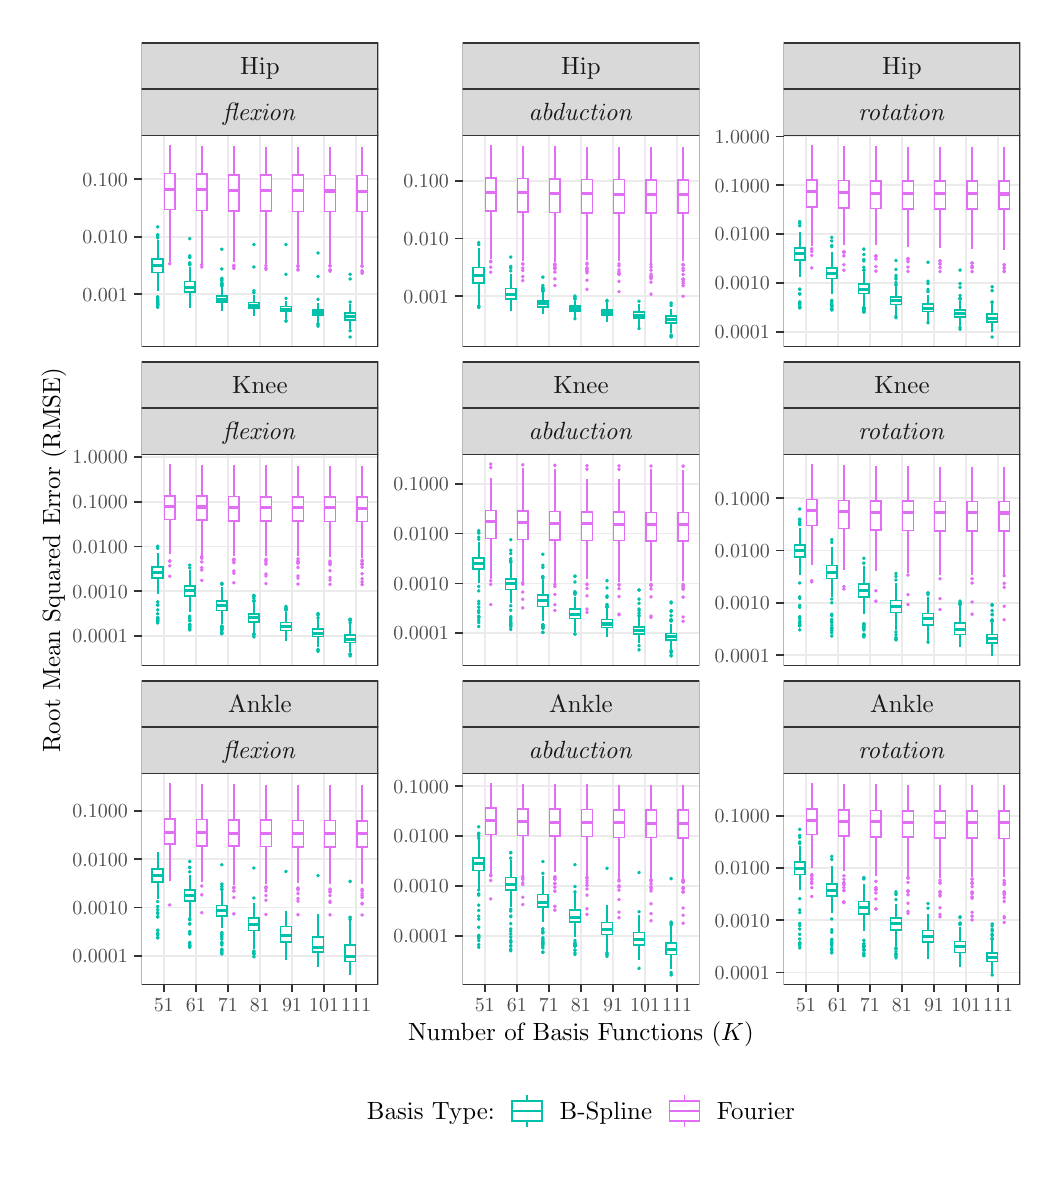
\begin{tikzpicture}[x=1pt,y=1pt]
\definecolor{fillColor}{RGB}{255,255,255}
\path[use as bounding box,fill=fillColor,fill opacity=0.00] (0,0) rectangle (364.19,409.72);
\begin{scope}
\path[clip] (  0.00,  0.00) rectangle (364.19,409.72);
\definecolor{drawColor}{RGB}{255,255,255}
\definecolor{fillColor}{RGB}{255,255,255}

\path[draw=drawColor,line width= 0.6pt,line join=round,line cap=round,fill=fillColor] (  0.00,  0.00) rectangle (364.19,409.72);
\end{scope}
\begin{scope}
\path[clip] ( 41.14,294.47) rectangle (126.70,370.72);
\definecolor{fillColor}{RGB}{255,255,255}

\path[fill=fillColor] ( 41.14,294.47) rectangle (126.70,370.72);
\definecolor{drawColor}{gray}{0.92}

\path[draw=drawColor,line width= 0.6pt,line join=round] ( 41.14,313.40) --
	(126.70,313.40);

\path[draw=drawColor,line width= 0.6pt,line join=round] ( 41.14,334.17) --
	(126.70,334.17);

\path[draw=drawColor,line width= 0.6pt,line join=round] ( 41.14,354.94) --
	(126.70,354.94);

\path[draw=drawColor,line width= 0.6pt,line join=round] ( 49.16,294.47) --
	( 49.16,370.72);

\path[draw=drawColor,line width= 0.6pt,line join=round] ( 60.75,294.47) --
	( 60.75,370.72);

\path[draw=drawColor,line width= 0.6pt,line join=round] ( 72.33,294.47) --
	( 72.33,370.72);

\path[draw=drawColor,line width= 0.6pt,line join=round] ( 83.92,294.47) --
	( 83.92,370.72);

\path[draw=drawColor,line width= 0.6pt,line join=round] ( 95.51,294.47) --
	( 95.51,370.72);

\path[draw=drawColor,line width= 0.6pt,line join=round] (107.09,294.47) --
	(107.09,370.72);

\path[draw=drawColor,line width= 0.6pt,line join=round] (118.68,294.47) --
	(118.68,370.72);
\definecolor{drawColor}{RGB}{0,193,169}
\definecolor{fillColor}{RGB}{0,193,169}

\path[draw=drawColor,line width= 0.4pt,line join=round,line cap=round,fill=fillColor] ( 46.99,310.56) circle (  0.46);

\path[draw=drawColor,line width= 0.4pt,line join=round,line cap=round,fill=fillColor] ( 46.99,334.89) circle (  0.46);

\path[draw=drawColor,line width= 0.4pt,line join=round,line cap=round,fill=fillColor] ( 46.99,333.76) circle (  0.46);

\path[draw=drawColor,line width= 0.4pt,line join=round,line cap=round,fill=fillColor] ( 46.99,310.35) circle (  0.46);

\path[draw=drawColor,line width= 0.4pt,line join=round,line cap=round,fill=fillColor] ( 46.99,334.46) circle (  0.46);

\path[draw=drawColor,line width= 0.4pt,line join=round,line cap=round,fill=fillColor] ( 46.99,308.67) circle (  0.46);

\path[draw=drawColor,line width= 0.4pt,line join=round,line cap=round,fill=fillColor] ( 46.99,310.19) circle (  0.46);

\path[draw=drawColor,line width= 0.4pt,line join=round,line cap=round,fill=fillColor] ( 46.99,309.66) circle (  0.46);

\path[draw=drawColor,line width= 0.4pt,line join=round,line cap=round,fill=fillColor] ( 46.99,312.00) circle (  0.46);

\path[draw=drawColor,line width= 0.4pt,line join=round,line cap=round,fill=fillColor] ( 46.99,309.83) circle (  0.46);

\path[draw=drawColor,line width= 0.4pt,line join=round,line cap=round,fill=fillColor] ( 46.99,309.21) circle (  0.46);

\path[draw=drawColor,line width= 0.4pt,line join=round,line cap=round,fill=fillColor] ( 46.99,311.18) circle (  0.46);

\path[draw=drawColor,line width= 0.4pt,line join=round,line cap=round,fill=fillColor] ( 46.99,311.78) circle (  0.46);

\path[draw=drawColor,line width= 0.4pt,line join=round,line cap=round,fill=fillColor] ( 46.99,337.74) circle (  0.46);

\path[draw=drawColor,line width= 0.4pt,line join=round,line cap=round,fill=fillColor] ( 46.99,312.47) circle (  0.46);

\path[draw=drawColor,line width= 0.4pt,line join=round,line cap=round,fill=fillColor] ( 46.99,311.11) circle (  0.46);

\path[draw=drawColor,line width= 0.4pt,line join=round,line cap=round,fill=fillColor] ( 46.99,309.64) circle (  0.46);

\path[draw=drawColor,line width= 0.6pt,line join=round] ( 46.99,326.04) -- ( 46.99,332.90);

\path[draw=drawColor,line width= 0.6pt,line join=round] ( 46.99,321.27) -- ( 46.99,314.50);
\definecolor{fillColor}{RGB}{255,255,255}

\path[draw=drawColor,line width= 0.6pt,fill=fillColor] ( 45.03,326.04) --
	( 45.03,321.27) --
	( 48.94,321.27) --
	( 48.94,326.04) --
	( 45.03,326.04) --
	cycle;

\path[draw=drawColor,line width= 1.1pt] ( 45.03,323.86) -- ( 48.94,323.86);
\definecolor{drawColor}{RGB}{227,110,246}
\definecolor{fillColor}{RGB}{227,110,246}

\path[draw=drawColor,line width= 0.4pt,line join=round,line cap=round,fill=fillColor] ( 51.33,324.40) circle (  0.46);

\path[draw=drawColor,line width= 0.6pt,line join=round] ( 51.33,356.99) -- ( 51.33,367.26);

\path[draw=drawColor,line width= 0.6pt,line join=round] ( 51.33,343.96) -- ( 51.33,324.96);
\definecolor{fillColor}{RGB}{255,255,255}

\path[draw=drawColor,line width= 0.6pt,fill=fillColor] ( 49.38,356.99) --
	( 49.38,343.96) --
	( 53.29,343.96) --
	( 53.29,356.99) --
	( 49.38,356.99) --
	cycle;

\path[draw=drawColor,line width= 1.1pt] ( 49.38,351.40) -- ( 53.29,351.40);
\definecolor{drawColor}{RGB}{0,193,169}
\definecolor{fillColor}{RGB}{0,193,169}

\path[draw=drawColor,line width= 0.4pt,line join=round,line cap=round,fill=fillColor] ( 58.57,324.74) circle (  0.46);

\path[draw=drawColor,line width= 0.4pt,line join=round,line cap=round,fill=fillColor] ( 58.57,326.86) circle (  0.46);

\path[draw=drawColor,line width= 0.4pt,line join=round,line cap=round,fill=fillColor] ( 58.57,324.09) circle (  0.46);

\path[draw=drawColor,line width= 0.4pt,line join=round,line cap=round,fill=fillColor] ( 58.57,324.15) circle (  0.46);

\path[draw=drawColor,line width= 0.4pt,line join=round,line cap=round,fill=fillColor] ( 58.57,326.64) circle (  0.46);

\path[draw=drawColor,line width= 0.4pt,line join=round,line cap=round,fill=fillColor] ( 58.57,333.50) circle (  0.46);

\path[draw=drawColor,line width= 0.4pt,line join=round,line cap=round,fill=fillColor] ( 58.57,327.25) circle (  0.46);

\path[draw=drawColor,line width= 0.4pt,line join=round,line cap=round,fill=fillColor] ( 58.57,324.47) circle (  0.46);

\path[draw=drawColor,line width= 0.6pt,line join=round] ( 58.57,317.96) -- ( 58.57,323.27);

\path[draw=drawColor,line width= 0.6pt,line join=round] ( 58.57,314.11) -- ( 58.57,308.39);
\definecolor{fillColor}{RGB}{255,255,255}

\path[draw=drawColor,line width= 0.6pt,fill=fillColor] ( 56.62,317.96) --
	( 56.62,314.11) --
	( 60.53,314.11) --
	( 60.53,317.96) --
	( 56.62,317.96) --
	cycle;

\path[draw=drawColor,line width= 1.1pt] ( 56.62,315.98) -- ( 60.53,315.98);
\definecolor{drawColor}{RGB}{227,110,246}
\definecolor{fillColor}{RGB}{227,110,246}

\path[draw=drawColor,line width= 0.4pt,line join=round,line cap=round,fill=fillColor] ( 62.92,323.23) circle (  0.46);

\path[draw=drawColor,line width= 0.4pt,line join=round,line cap=round,fill=fillColor] ( 62.92,324.07) circle (  0.46);

\path[draw=drawColor,line width= 0.6pt,line join=round] ( 62.92,356.73) -- ( 62.92,367.01);

\path[draw=drawColor,line width= 0.6pt,line join=round] ( 62.92,343.68) -- ( 62.92,324.49);
\definecolor{fillColor}{RGB}{255,255,255}

\path[draw=drawColor,line width= 0.6pt,fill=fillColor] ( 60.96,356.73) --
	( 60.96,343.68) --
	( 64.87,343.68) --
	( 64.87,356.73) --
	( 60.96,356.73) --
	cycle;

\path[draw=drawColor,line width= 1.1pt] ( 60.96,351.12) -- ( 64.87,351.12);
\definecolor{drawColor}{RGB}{0,193,169}
\definecolor{fillColor}{RGB}{0,193,169}

\path[draw=drawColor,line width= 0.4pt,line join=round,line cap=round,fill=fillColor] ( 70.16,318.26) circle (  0.46);

\path[draw=drawColor,line width= 0.4pt,line join=round,line cap=round,fill=fillColor] ( 70.16,318.80) circle (  0.46);

\path[draw=drawColor,line width= 0.4pt,line join=round,line cap=round,fill=fillColor] ( 70.16,316.59) circle (  0.46);

\path[draw=drawColor,line width= 0.4pt,line join=round,line cap=round,fill=fillColor] ( 70.16,317.41) circle (  0.46);

\path[draw=drawColor,line width= 0.4pt,line join=round,line cap=round,fill=fillColor] ( 70.16,317.30) circle (  0.46);

\path[draw=drawColor,line width= 0.4pt,line join=round,line cap=round,fill=fillColor] ( 70.16,319.16) circle (  0.46);

\path[draw=drawColor,line width= 0.4pt,line join=round,line cap=round,fill=fillColor] ( 70.16,316.88) circle (  0.46);

\path[draw=drawColor,line width= 0.4pt,line join=round,line cap=round,fill=fillColor] ( 70.16,329.68) circle (  0.46);

\path[draw=drawColor,line width= 0.4pt,line join=round,line cap=round,fill=fillColor] ( 70.16,322.54) circle (  0.46);

\path[draw=drawColor,line width= 0.4pt,line join=round,line cap=round,fill=fillColor] ( 70.16,316.42) circle (  0.46);

\path[draw=drawColor,line width= 0.6pt,line join=round] ( 70.16,312.84) -- ( 70.16,316.25);

\path[draw=drawColor,line width= 0.6pt,line join=round] ( 70.16,310.52) -- ( 70.16,307.26);
\definecolor{fillColor}{RGB}{255,255,255}

\path[draw=drawColor,line width= 0.6pt,fill=fillColor] ( 68.21,312.84) --
	( 68.21,310.52) --
	( 72.12,310.52) --
	( 72.12,312.84) --
	( 68.21,312.84) --
	cycle;

\path[draw=drawColor,line width= 1.1pt] ( 68.21,311.58) -- ( 72.12,311.58);
\definecolor{drawColor}{RGB}{227,110,246}
\definecolor{fillColor}{RGB}{227,110,246}

\path[draw=drawColor,line width= 0.4pt,line join=round,line cap=round,fill=fillColor] ( 74.51,322.73) circle (  0.46);

\path[draw=drawColor,line width= 0.4pt,line join=round,line cap=round,fill=fillColor] ( 74.51,323.50) circle (  0.46);

\path[draw=drawColor,line width= 0.4pt,line join=round,line cap=round,fill=fillColor] ( 74.51,323.89) circle (  0.46);

\path[draw=drawColor,line width= 0.6pt,line join=round] ( 74.51,356.56) -- ( 74.51,366.86);

\path[draw=drawColor,line width= 0.6pt,line join=round] ( 74.51,343.52) -- ( 74.51,325.17);
\definecolor{fillColor}{RGB}{255,255,255}

\path[draw=drawColor,line width= 0.6pt,fill=fillColor] ( 72.55,356.56) --
	( 72.55,343.52) --
	( 76.46,343.52) --
	( 76.46,356.56) --
	( 72.55,356.56) --
	cycle;

\path[draw=drawColor,line width= 1.1pt] ( 72.55,350.93) -- ( 76.46,350.93);
\definecolor{drawColor}{RGB}{0,193,169}
\definecolor{fillColor}{RGB}{0,193,169}

\path[draw=drawColor,line width= 0.4pt,line join=round,line cap=round,fill=fillColor] ( 81.75,313.98) circle (  0.46);

\path[draw=drawColor,line width= 0.4pt,line join=round,line cap=round,fill=fillColor] ( 81.75,314.63) circle (  0.46);

\path[draw=drawColor,line width= 0.4pt,line join=round,line cap=round,fill=fillColor] ( 81.75,331.35) circle (  0.46);

\path[draw=drawColor,line width= 0.4pt,line join=round,line cap=round,fill=fillColor] ( 81.75,323.25) circle (  0.46);

\path[draw=drawColor,line width= 0.6pt,line join=round] ( 81.75,310.35) -- ( 81.75,313.28);

\path[draw=drawColor,line width= 0.6pt,line join=round] ( 81.75,308.33) -- ( 81.75,305.37);
\definecolor{fillColor}{RGB}{255,255,255}

\path[draw=drawColor,line width= 0.6pt,fill=fillColor] ( 79.79,310.35) --
	( 79.79,308.33) --
	( 83.70,308.33) --
	( 83.70,310.35) --
	( 79.79,310.35) --
	cycle;

\path[draw=drawColor,line width= 1.1pt] ( 79.79,309.49) -- ( 83.70,309.49);
\definecolor{drawColor}{RGB}{227,110,246}
\definecolor{fillColor}{RGB}{227,110,246}

\path[draw=drawColor,line width= 0.4pt,line join=round,line cap=round,fill=fillColor] ( 86.09,322.41) circle (  0.46);

\path[draw=drawColor,line width= 0.4pt,line join=round,line cap=round,fill=fillColor] ( 86.09,322.86) circle (  0.46);

\path[draw=drawColor,line width= 0.4pt,line join=round,line cap=round,fill=fillColor] ( 86.09,323.78) circle (  0.46);

\path[draw=drawColor,line width= 0.6pt,line join=round] ( 86.09,356.44) -- ( 86.09,366.76);

\path[draw=drawColor,line width= 0.6pt,line join=round] ( 86.09,343.40) -- ( 86.09,324.44);
\definecolor{fillColor}{RGB}{255,255,255}

\path[draw=drawColor,line width= 0.6pt,fill=fillColor] ( 84.14,356.44) --
	( 84.14,343.40) --
	( 88.05,343.40) --
	( 88.05,356.44) --
	( 84.14,356.44) --
	cycle;

\path[draw=drawColor,line width= 1.1pt] ( 84.14,350.81) -- ( 88.05,350.81);
\definecolor{drawColor}{RGB}{0,193,169}
\definecolor{fillColor}{RGB}{0,193,169}

\path[draw=drawColor,line width= 0.4pt,line join=round,line cap=round,fill=fillColor] ( 93.33,311.89) circle (  0.46);

\path[draw=drawColor,line width= 0.4pt,line join=round,line cap=round,fill=fillColor] ( 93.33,303.68) circle (  0.46);

\path[draw=drawColor,line width= 0.4pt,line join=round,line cap=round,fill=fillColor] ( 93.33,303.76) circle (  0.46);

\path[draw=drawColor,line width= 0.4pt,line join=round,line cap=round,fill=fillColor] ( 93.33,331.34) circle (  0.46);

\path[draw=drawColor,line width= 0.4pt,line join=round,line cap=round,fill=fillColor] ( 93.33,320.60) circle (  0.46);

\path[draw=drawColor,line width= 0.6pt,line join=round] ( 93.33,308.96) -- ( 93.33,311.10);

\path[draw=drawColor,line width= 0.6pt,line join=round] ( 93.33,307.14) -- ( 93.33,304.47);
\definecolor{fillColor}{RGB}{255,255,255}

\path[draw=drawColor,line width= 0.6pt,fill=fillColor] ( 91.38,308.96) --
	( 91.38,307.14) --
	( 95.29,307.14) --
	( 95.29,308.96) --
	( 91.38,308.96) --
	cycle;

\path[draw=drawColor,line width= 1.1pt] ( 91.38,308.02) -- ( 95.29,308.02);
\definecolor{drawColor}{RGB}{227,110,246}
\definecolor{fillColor}{RGB}{227,110,246}

\path[draw=drawColor,line width= 0.4pt,line join=round,line cap=round,fill=fillColor] ( 97.68,322.29) circle (  0.46);

\path[draw=drawColor,line width= 0.4pt,line join=round,line cap=round,fill=fillColor] ( 97.68,322.21) circle (  0.46);

\path[draw=drawColor,line width= 0.4pt,line join=round,line cap=round,fill=fillColor] ( 97.68,323.68) circle (  0.46);

\path[draw=drawColor,line width= 0.4pt,line join=round,line cap=round,fill=fillColor] ( 97.68,323.40) circle (  0.46);

\path[draw=drawColor,line width= 0.6pt,line join=round] ( 97.68,356.36) -- ( 97.68,366.70);

\path[draw=drawColor,line width= 0.6pt,line join=round] ( 97.68,343.34) -- ( 97.68,323.98);
\definecolor{fillColor}{RGB}{255,255,255}

\path[draw=drawColor,line width= 0.6pt,fill=fillColor] ( 95.72,356.36) --
	( 95.72,343.34) --
	( 99.63,343.34) --
	( 99.63,356.36) --
	( 95.72,356.36) --
	cycle;

\path[draw=drawColor,line width= 1.1pt] ( 95.72,350.74) -- ( 99.63,350.74);
\definecolor{drawColor}{RGB}{0,193,169}
\definecolor{fillColor}{RGB}{0,193,169}

\path[draw=drawColor,line width= 0.4pt,line join=round,line cap=round,fill=fillColor] (104.92,302.34) circle (  0.46);

\path[draw=drawColor,line width= 0.4pt,line join=round,line cap=round,fill=fillColor] (104.92,311.54) circle (  0.46);

\path[draw=drawColor,line width= 0.4pt,line join=round,line cap=round,fill=fillColor] (104.92,302.78) circle (  0.46);

\path[draw=drawColor,line width= 0.4pt,line join=round,line cap=round,fill=fillColor] (104.92,301.86) circle (  0.46);

\path[draw=drawColor,line width= 0.4pt,line join=round,line cap=round,fill=fillColor] (104.92,328.31) circle (  0.46);

\path[draw=drawColor,line width= 0.4pt,line join=round,line cap=round,fill=fillColor] (104.92,319.82) circle (  0.46);

\path[draw=drawColor,line width= 0.6pt,line join=round] (104.92,307.80) -- (104.92,310.36);

\path[draw=drawColor,line width= 0.6pt,line join=round] (104.92,305.90) -- (104.92,303.11);
\definecolor{fillColor}{RGB}{255,255,255}

\path[draw=drawColor,line width= 0.6pt,fill=fillColor] (102.97,307.80) --
	(102.97,305.90) --
	(106.88,305.90) --
	(106.88,307.80) --
	(102.97,307.80) --
	cycle;

\path[draw=drawColor,line width= 1.1pt] (102.97,306.79) -- (106.88,306.79);
\definecolor{drawColor}{RGB}{227,110,246}
\definecolor{fillColor}{RGB}{227,110,246}

\path[draw=drawColor,line width= 0.4pt,line join=round,line cap=round,fill=fillColor] (109.27,323.73) circle (  0.46);

\path[draw=drawColor,line width= 0.4pt,line join=round,line cap=round,fill=fillColor] (109.27,322.14) circle (  0.46);

\path[draw=drawColor,line width= 0.4pt,line join=round,line cap=round,fill=fillColor] (109.27,321.71) circle (  0.46);

\path[draw=drawColor,line width= 0.4pt,line join=round,line cap=round,fill=fillColor] (109.27,323.63) circle (  0.46);

\path[draw=drawColor,line width= 0.4pt,line join=round,line cap=round,fill=fillColor] (109.27,322.12) circle (  0.46);

\path[draw=drawColor,line width= 0.6pt,line join=round] (109.27,356.31) -- (109.27,366.66);

\path[draw=drawColor,line width= 0.6pt,line join=round] (109.27,343.30) -- (109.27,324.11);
\definecolor{fillColor}{RGB}{255,255,255}

\path[draw=drawColor,line width= 0.6pt,fill=fillColor] (107.31,356.31) --
	(107.31,343.30) --
	(111.22,343.30) --
	(111.22,356.31) --
	(107.31,356.31) --
	cycle;

\path[draw=drawColor,line width= 1.1pt] (107.31,350.69) -- (111.22,350.69);
\definecolor{drawColor}{RGB}{0,193,169}
\definecolor{fillColor}{RGB}{0,193,169}

\path[draw=drawColor,line width= 0.4pt,line join=round,line cap=round,fill=fillColor] (116.51,300.20) circle (  0.46);

\path[draw=drawColor,line width= 0.4pt,line join=round,line cap=round,fill=fillColor] (116.51,297.93) circle (  0.46);

\path[draw=drawColor,line width= 0.4pt,line join=round,line cap=round,fill=fillColor] (116.51,310.58) circle (  0.46);

\path[draw=drawColor,line width= 0.4pt,line join=round,line cap=round,fill=fillColor] (116.51,320.61) circle (  0.46);

\path[draw=drawColor,line width= 0.4pt,line join=round,line cap=round,fill=fillColor] (116.51,318.89) circle (  0.46);

\path[draw=drawColor,line width= 0.6pt,line join=round] (116.51,306.59) -- (116.51,309.75);

\path[draw=drawColor,line width= 0.6pt,line join=round] (116.51,304.17) -- (116.51,300.84);
\definecolor{fillColor}{RGB}{255,255,255}

\path[draw=drawColor,line width= 0.6pt,fill=fillColor] (114.55,306.59) --
	(114.55,304.17) --
	(118.46,304.17) --
	(118.46,306.59) --
	(114.55,306.59) --
	cycle;

\path[draw=drawColor,line width= 1.1pt] (114.55,305.37) -- (118.46,305.37);
\definecolor{drawColor}{RGB}{227,110,246}
\definecolor{fillColor}{RGB}{227,110,246}

\path[draw=drawColor,line width= 0.4pt,line join=round,line cap=round,fill=fillColor] (120.85,323.53) circle (  0.46);

\path[draw=drawColor,line width= 0.4pt,line join=round,line cap=round,fill=fillColor] (120.85,321.90) circle (  0.46);

\path[draw=drawColor,line width= 0.4pt,line join=round,line cap=round,fill=fillColor] (120.85,321.51) circle (  0.46);

\path[draw=drawColor,line width= 0.4pt,line join=round,line cap=round,fill=fillColor] (120.85,323.59) circle (  0.46);

\path[draw=drawColor,line width= 0.4pt,line join=round,line cap=round,fill=fillColor] (120.85,321.03) circle (  0.46);

\path[draw=drawColor,line width= 0.6pt,line join=round] (120.85,356.28) -- (120.85,366.65);

\path[draw=drawColor,line width= 0.6pt,line join=round] (120.85,343.28) -- (120.85,323.91);
\definecolor{fillColor}{RGB}{255,255,255}

\path[draw=drawColor,line width= 0.6pt,fill=fillColor] (118.90,356.28) --
	(118.90,343.28) --
	(122.81,343.28) --
	(122.81,356.28) --
	(118.90,356.28) --
	cycle;

\path[draw=drawColor,line width= 1.1pt] (118.90,350.67) -- (122.81,350.67);
\definecolor{drawColor}{gray}{0.20}

\path[draw=drawColor,line width= 0.6pt,line join=round,line cap=round] ( 41.14,294.47) rectangle (126.70,370.72);
\end{scope}
\begin{scope}
\path[clip] ( 41.14,179.21) rectangle (126.70,255.47);
\definecolor{fillColor}{RGB}{255,255,255}

\path[fill=fillColor] ( 41.14,179.21) rectangle (126.70,255.47);
\definecolor{drawColor}{gray}{0.92}

\path[draw=drawColor,line width= 0.6pt,line join=round] ( 41.14,189.90) --
	(126.70,189.90);

\path[draw=drawColor,line width= 0.6pt,line join=round] ( 41.14,206.07) --
	(126.70,206.07);

\path[draw=drawColor,line width= 0.6pt,line join=round] ( 41.14,222.24) --
	(126.70,222.24);

\path[draw=drawColor,line width= 0.6pt,line join=round] ( 41.14,238.40) --
	(126.70,238.40);

\path[draw=drawColor,line width= 0.6pt,line join=round] ( 41.14,254.57) --
	(126.70,254.57);

\path[draw=drawColor,line width= 0.6pt,line join=round] ( 49.16,179.21) --
	( 49.16,255.47);

\path[draw=drawColor,line width= 0.6pt,line join=round] ( 60.75,179.21) --
	( 60.75,255.47);

\path[draw=drawColor,line width= 0.6pt,line join=round] ( 72.33,179.21) --
	( 72.33,255.47);

\path[draw=drawColor,line width= 0.6pt,line join=round] ( 83.92,179.21) --
	( 83.92,255.47);

\path[draw=drawColor,line width= 0.6pt,line join=round] ( 95.51,179.21) --
	( 95.51,255.47);

\path[draw=drawColor,line width= 0.6pt,line join=round] (107.09,179.21) --
	(107.09,255.47);

\path[draw=drawColor,line width= 0.6pt,line join=round] (118.68,179.21) --
	(118.68,255.47);
\definecolor{drawColor}{RGB}{0,193,169}
\definecolor{fillColor}{RGB}{0,193,169}

\path[draw=drawColor,line width= 0.4pt,line join=round,line cap=round,fill=fillColor] ( 46.99,196.32) circle (  0.46);

\path[draw=drawColor,line width= 0.4pt,line join=round,line cap=round,fill=fillColor] ( 46.99,202.22) circle (  0.46);

\path[draw=drawColor,line width= 0.4pt,line join=round,line cap=round,fill=fillColor] ( 46.99,222.35) circle (  0.46);

\path[draw=drawColor,line width= 0.4pt,line join=round,line cap=round,fill=fillColor] ( 46.99,221.59) circle (  0.46);

\path[draw=drawColor,line width= 0.4pt,line join=round,line cap=round,fill=fillColor] ( 46.99,195.46) circle (  0.46);

\path[draw=drawColor,line width= 0.4pt,line join=round,line cap=round,fill=fillColor] ( 46.99,195.70) circle (  0.46);

\path[draw=drawColor,line width= 0.4pt,line join=round,line cap=round,fill=fillColor] ( 46.99,195.10) circle (  0.46);

\path[draw=drawColor,line width= 0.4pt,line join=round,line cap=round,fill=fillColor] ( 46.99,201.02) circle (  0.46);

\path[draw=drawColor,line width= 0.4pt,line join=round,line cap=round,fill=fillColor] ( 46.99,196.49) circle (  0.46);

\path[draw=drawColor,line width= 0.4pt,line join=round,line cap=round,fill=fillColor] ( 46.99,194.61) circle (  0.46);

\path[draw=drawColor,line width= 0.4pt,line join=round,line cap=round,fill=fillColor] ( 46.99,196.49) circle (  0.46);

\path[draw=drawColor,line width= 0.4pt,line join=round,line cap=round,fill=fillColor] ( 46.99,195.62) circle (  0.46);

\path[draw=drawColor,line width= 0.4pt,line join=round,line cap=round,fill=fillColor] ( 46.99,199.35) circle (  0.46);

\path[draw=drawColor,line width= 0.4pt,line join=round,line cap=round,fill=fillColor] ( 46.99,201.20) circle (  0.46);

\path[draw=drawColor,line width= 0.4pt,line join=round,line cap=round,fill=fillColor] ( 46.99,197.93) circle (  0.46);

\path[draw=drawColor,line width= 0.6pt,line join=round] ( 46.99,214.77) -- ( 46.99,220.04);

\path[draw=drawColor,line width= 0.6pt,line join=round] ( 46.99,210.83) -- ( 46.99,205.03);
\definecolor{fillColor}{RGB}{255,255,255}

\path[draw=drawColor,line width= 0.6pt,fill=fillColor] ( 45.03,214.77) --
	( 45.03,210.83) --
	( 48.94,210.83) --
	( 48.94,214.77) --
	( 45.03,214.77) --
	cycle;

\path[draw=drawColor,line width= 1.1pt] ( 45.03,212.98) -- ( 48.94,212.98);
\definecolor{drawColor}{RGB}{227,110,246}
\definecolor{fillColor}{RGB}{227,110,246}

\path[draw=drawColor,line width= 0.4pt,line join=round,line cap=round,fill=fillColor] ( 51.33,211.48) circle (  0.46);

\path[draw=drawColor,line width= 0.4pt,line join=round,line cap=round,fill=fillColor] ( 51.33,216.92) circle (  0.46);

\path[draw=drawColor,line width= 0.4pt,line join=round,line cap=round,fill=fillColor] ( 51.33,217.04) circle (  0.46);

\path[draw=drawColor,line width= 0.4pt,line join=round,line cap=round,fill=fillColor] ( 51.33,215.25) circle (  0.46);

\path[draw=drawColor,line width= 0.6pt,line join=round] ( 51.33,240.58) -- ( 51.33,252.00);

\path[draw=drawColor,line width= 0.6pt,line join=round] ( 51.33,232.04) -- ( 51.33,219.50);
\definecolor{fillColor}{RGB}{255,255,255}

\path[draw=drawColor,line width= 0.6pt,fill=fillColor] ( 49.38,240.58) --
	( 49.38,232.04) --
	( 53.29,232.04) --
	( 53.29,240.58) --
	( 49.38,240.58) --
	cycle;

\path[draw=drawColor,line width= 1.1pt] ( 49.38,236.71) -- ( 53.29,236.71);
\definecolor{drawColor}{RGB}{0,193,169}
\definecolor{fillColor}{RGB}{0,193,169}

\path[draw=drawColor,line width= 0.4pt,line join=round,line cap=round,fill=fillColor] ( 58.57,193.75) circle (  0.46);

\path[draw=drawColor,line width= 0.4pt,line join=round,line cap=round,fill=fillColor] ( 58.57,214.52) circle (  0.46);

\path[draw=drawColor,line width= 0.4pt,line join=round,line cap=round,fill=fillColor] ( 58.57,197.05) circle (  0.46);

\path[draw=drawColor,line width= 0.4pt,line join=round,line cap=round,fill=fillColor] ( 58.57,215.51) circle (  0.46);

\path[draw=drawColor,line width= 0.4pt,line join=round,line cap=round,fill=fillColor] ( 58.57,194.09) circle (  0.46);

\path[draw=drawColor,line width= 0.4pt,line join=round,line cap=round,fill=fillColor] ( 58.57,193.33) circle (  0.46);

\path[draw=drawColor,line width= 0.4pt,line join=round,line cap=round,fill=fillColor] ( 58.57,192.26) circle (  0.46);

\path[draw=drawColor,line width= 0.4pt,line join=round,line cap=round,fill=fillColor] ( 58.57,195.57) circle (  0.46);

\path[draw=drawColor,line width= 0.4pt,line join=round,line cap=round,fill=fillColor] ( 58.57,195.53) circle (  0.46);

\path[draw=drawColor,line width= 0.4pt,line join=round,line cap=round,fill=fillColor] ( 58.57,192.68) circle (  0.46);

\path[draw=drawColor,line width= 0.4pt,line join=round,line cap=round,fill=fillColor] ( 58.57,193.95) circle (  0.46);

\path[draw=drawColor,line width= 0.4pt,line join=round,line cap=round,fill=fillColor] ( 58.57,192.12) circle (  0.46);

\path[draw=drawColor,line width= 0.4pt,line join=round,line cap=round,fill=fillColor] ( 58.57,195.45) circle (  0.46);

\path[draw=drawColor,line width= 0.4pt,line join=round,line cap=round,fill=fillColor] ( 58.57,196.37) circle (  0.46);

\path[draw=drawColor,line width= 0.4pt,line join=round,line cap=round,fill=fillColor] ( 58.57,193.00) circle (  0.46);

\path[draw=drawColor,line width= 0.6pt,line join=round] ( 58.57,208.05) -- ( 58.57,213.66);

\path[draw=drawColor,line width= 0.6pt,line join=round] ( 58.57,204.26) -- ( 58.57,198.70);
\definecolor{fillColor}{RGB}{255,255,255}

\path[draw=drawColor,line width= 0.6pt,fill=fillColor] ( 56.62,208.05) --
	( 56.62,204.26) --
	( 60.53,204.26) --
	( 60.53,208.05) --
	( 56.62,208.05) --
	cycle;

\path[draw=drawColor,line width= 1.1pt] ( 56.62,206.30) -- ( 60.53,206.30);
\definecolor{drawColor}{RGB}{227,110,246}
\definecolor{fillColor}{RGB}{227,110,246}

\path[draw=drawColor,line width= 0.4pt,line join=round,line cap=round,fill=fillColor] ( 62.92,209.98) circle (  0.46);

\path[draw=drawColor,line width= 0.4pt,line join=round,line cap=round,fill=fillColor] ( 62.92,218.59) circle (  0.46);

\path[draw=drawColor,line width= 0.4pt,line join=round,line cap=round,fill=fillColor] ( 62.92,218.58) circle (  0.46);

\path[draw=drawColor,line width= 0.4pt,line join=round,line cap=round,fill=fillColor] ( 62.92,214.60) circle (  0.46);

\path[draw=drawColor,line width= 0.4pt,line join=round,line cap=round,fill=fillColor] ( 62.92,218.02) circle (  0.46);

\path[draw=drawColor,line width= 0.4pt,line join=round,line cap=round,fill=fillColor] ( 62.92,216.65) circle (  0.46);

\path[draw=drawColor,line width= 0.4pt,line join=round,line cap=round,fill=fillColor] ( 62.92,213.74) circle (  0.46);

\path[draw=drawColor,line width= 0.6pt,line join=round] ( 62.92,240.37) -- ( 62.92,251.79);

\path[draw=drawColor,line width= 0.6pt,line join=round] ( 62.92,231.74) -- ( 62.92,219.21);
\definecolor{fillColor}{RGB}{255,255,255}

\path[draw=drawColor,line width= 0.6pt,fill=fillColor] ( 60.96,240.37) --
	( 60.96,231.74) --
	( 64.87,231.74) --
	( 64.87,240.37) --
	( 60.96,240.37) --
	cycle;

\path[draw=drawColor,line width= 1.1pt] ( 60.96,236.51) -- ( 64.87,236.51);
\definecolor{drawColor}{RGB}{0,193,169}
\definecolor{fillColor}{RGB}{0,193,169}

\path[draw=drawColor,line width= 0.4pt,line join=round,line cap=round,fill=fillColor] ( 70.16,208.77) circle (  0.46);

\path[draw=drawColor,line width= 0.4pt,line join=round,line cap=round,fill=fillColor] ( 70.16,193.46) circle (  0.46);

\path[draw=drawColor,line width= 0.4pt,line join=round,line cap=round,fill=fillColor] ( 70.16,208.62) circle (  0.46);

\path[draw=drawColor,line width= 0.4pt,line join=round,line cap=round,fill=fillColor] ( 70.16,208.94) circle (  0.46);

\path[draw=drawColor,line width= 0.4pt,line join=round,line cap=round,fill=fillColor] ( 70.16,193.23) circle (  0.46);

\path[draw=drawColor,line width= 0.4pt,line join=round,line cap=round,fill=fillColor] ( 70.16,193.27) circle (  0.46);

\path[draw=drawColor,line width= 0.4pt,line join=round,line cap=round,fill=fillColor] ( 70.16,193.39) circle (  0.46);

\path[draw=drawColor,line width= 0.4pt,line join=round,line cap=round,fill=fillColor] ( 70.16,191.94) circle (  0.46);

\path[draw=drawColor,line width= 0.4pt,line join=round,line cap=round,fill=fillColor] ( 70.16,192.42) circle (  0.46);

\path[draw=drawColor,line width= 0.4pt,line join=round,line cap=round,fill=fillColor] ( 70.16,190.70) circle (  0.46);

\path[draw=drawColor,line width= 0.4pt,line join=round,line cap=round,fill=fillColor] ( 70.16,192.50) circle (  0.46);

\path[draw=drawColor,line width= 0.4pt,line join=round,line cap=round,fill=fillColor] ( 70.16,190.84) circle (  0.46);

\path[draw=drawColor,line width= 0.4pt,line join=round,line cap=round,fill=fillColor] ( 70.16,192.98) circle (  0.46);

\path[draw=drawColor,line width= 0.4pt,line join=round,line cap=round,fill=fillColor] ( 70.16,192.50) circle (  0.46);

\path[draw=drawColor,line width= 0.4pt,line join=round,line cap=round,fill=fillColor] ( 70.16,191.27) circle (  0.46);

\path[draw=drawColor,line width= 0.6pt,line join=round] ( 70.16,202.66) -- ( 70.16,207.61);

\path[draw=drawColor,line width= 0.6pt,line join=round] ( 70.16,199.13) -- ( 70.16,194.29);
\definecolor{fillColor}{RGB}{255,255,255}

\path[draw=drawColor,line width= 0.6pt,fill=fillColor] ( 68.21,202.66) --
	( 68.21,199.13) --
	( 72.12,199.13) --
	( 72.12,202.66) --
	( 68.21,202.66) --
	cycle;

\path[draw=drawColor,line width= 1.1pt] ( 68.21,200.94) -- ( 72.12,200.94);
\definecolor{drawColor}{RGB}{227,110,246}
\definecolor{fillColor}{RGB}{227,110,246}

\path[draw=drawColor,line width= 0.4pt,line join=round,line cap=round,fill=fillColor] ( 74.51,209.14) circle (  0.46);

\path[draw=drawColor,line width= 0.4pt,line join=round,line cap=round,fill=fillColor] ( 74.51,217.13) circle (  0.46);

\path[draw=drawColor,line width= 0.4pt,line join=round,line cap=round,fill=fillColor] ( 74.51,217.65) circle (  0.46);

\path[draw=drawColor,line width= 0.4pt,line join=round,line cap=round,fill=fillColor] ( 74.51,213.40) circle (  0.46);

\path[draw=drawColor,line width= 0.4pt,line join=round,line cap=round,fill=fillColor] ( 74.51,217.59) circle (  0.46);

\path[draw=drawColor,line width= 0.4pt,line join=round,line cap=round,fill=fillColor] ( 74.51,216.40) circle (  0.46);

\path[draw=drawColor,line width= 0.4pt,line join=round,line cap=round,fill=fillColor] ( 74.51,212.58) circle (  0.46);

\path[draw=drawColor,line width= 0.6pt,line join=round] ( 74.51,240.26) -- ( 74.51,251.64);

\path[draw=drawColor,line width= 0.6pt,line join=round] ( 74.51,231.57) -- ( 74.51,218.84);
\definecolor{fillColor}{RGB}{255,255,255}

\path[draw=drawColor,line width= 0.6pt,fill=fillColor] ( 72.55,240.26) --
	( 72.55,231.57) --
	( 76.46,231.57) --
	( 76.46,240.26) --
	( 72.55,240.26) --
	cycle;

\path[draw=drawColor,line width= 1.1pt] ( 72.55,236.39) -- ( 76.46,236.39);
\definecolor{drawColor}{RGB}{0,193,169}
\definecolor{fillColor}{RGB}{0,193,169}

\path[draw=drawColor,line width= 0.4pt,line join=round,line cap=round,fill=fillColor] ( 81.75,204.60) circle (  0.46);

\path[draw=drawColor,line width= 0.4pt,line join=round,line cap=round,fill=fillColor] ( 81.75,202.41) circle (  0.46);

\path[draw=drawColor,line width= 0.4pt,line join=round,line cap=round,fill=fillColor] ( 81.75,204.12) circle (  0.46);

\path[draw=drawColor,line width= 0.4pt,line join=round,line cap=round,fill=fillColor] ( 81.75,190.56) circle (  0.46);

\path[draw=drawColor,line width= 0.4pt,line join=round,line cap=round,fill=fillColor] ( 81.75,204.38) circle (  0.46);

\path[draw=drawColor,line width= 0.4pt,line join=round,line cap=round,fill=fillColor] ( 81.75,202.63) circle (  0.46);

\path[draw=drawColor,line width= 0.4pt,line join=round,line cap=round,fill=fillColor] ( 81.75,203.43) circle (  0.46);

\path[draw=drawColor,line width= 0.4pt,line join=round,line cap=round,fill=fillColor] ( 81.75,190.48) circle (  0.46);

\path[draw=drawColor,line width= 0.4pt,line join=round,line cap=round,fill=fillColor] ( 81.75,190.36) circle (  0.46);

\path[draw=drawColor,line width= 0.4pt,line join=round,line cap=round,fill=fillColor] ( 81.75,190.62) circle (  0.46);

\path[draw=drawColor,line width= 0.4pt,line join=round,line cap=round,fill=fillColor] ( 81.75,202.63) circle (  0.46);

\path[draw=drawColor,line width= 0.4pt,line join=round,line cap=round,fill=fillColor] ( 81.75,189.59) circle (  0.46);

\path[draw=drawColor,line width= 0.6pt,line join=round] ( 81.75,197.94) -- ( 81.75,201.74);

\path[draw=drawColor,line width= 0.6pt,line join=round] ( 81.75,195.04) -- ( 81.75,190.81);
\definecolor{fillColor}{RGB}{255,255,255}

\path[draw=drawColor,line width= 0.6pt,fill=fillColor] ( 79.79,197.94) --
	( 79.79,195.04) --
	( 83.70,195.04) --
	( 83.70,197.94) --
	( 79.79,197.94) --
	cycle;

\path[draw=drawColor,line width= 1.1pt] ( 79.79,196.46) -- ( 83.70,196.46);
\definecolor{drawColor}{RGB}{227,110,246}
\definecolor{fillColor}{RGB}{227,110,246}

\path[draw=drawColor,line width= 0.4pt,line join=round,line cap=round,fill=fillColor] ( 86.09,208.86) circle (  0.46);

\path[draw=drawColor,line width= 0.4pt,line join=round,line cap=round,fill=fillColor] ( 86.09,215.82) circle (  0.46);

\path[draw=drawColor,line width= 0.4pt,line join=round,line cap=round,fill=fillColor] ( 86.09,216.99) circle (  0.46);

\path[draw=drawColor,line width= 0.4pt,line join=round,line cap=round,fill=fillColor] ( 86.09,212.32) circle (  0.46);

\path[draw=drawColor,line width= 0.4pt,line join=round,line cap=round,fill=fillColor] ( 86.09,217.27) circle (  0.46);

\path[draw=drawColor,line width= 0.4pt,line join=round,line cap=round,fill=fillColor] ( 86.09,216.26) circle (  0.46);

\path[draw=drawColor,line width= 0.4pt,line join=round,line cap=round,fill=fillColor] ( 86.09,217.67) circle (  0.46);

\path[draw=drawColor,line width= 0.4pt,line join=round,line cap=round,fill=fillColor] ( 86.09,211.60) circle (  0.46);

\path[draw=drawColor,line width= 0.6pt,line join=round] ( 86.09,240.15) -- ( 86.09,251.55);

\path[draw=drawColor,line width= 0.6pt,line join=round] ( 86.09,231.45) -- ( 86.09,218.86);
\definecolor{fillColor}{RGB}{255,255,255}

\path[draw=drawColor,line width= 0.6pt,fill=fillColor] ( 84.14,240.15) --
	( 84.14,231.45) --
	( 88.05,231.45) --
	( 88.05,240.15) --
	( 84.14,240.15) --
	cycle;

\path[draw=drawColor,line width= 1.1pt] ( 84.14,236.31) -- ( 88.05,236.31);
\definecolor{drawColor}{RGB}{0,193,169}
\definecolor{fillColor}{RGB}{0,193,169}

\path[draw=drawColor,line width= 0.4pt,line join=round,line cap=round,fill=fillColor] ( 93.33,199.94) circle (  0.46);

\path[draw=drawColor,line width= 0.4pt,line join=round,line cap=round,fill=fillColor] ( 93.33,199.49) circle (  0.46);

\path[draw=drawColor,line width= 0.4pt,line join=round,line cap=round,fill=fillColor] ( 93.33,199.29) circle (  0.46);

\path[draw=drawColor,line width= 0.4pt,line join=round,line cap=round,fill=fillColor] ( 93.33,200.17) circle (  0.46);

\path[draw=drawColor,line width= 0.4pt,line join=round,line cap=round,fill=fillColor] ( 93.33,199.58) circle (  0.46);

\path[draw=drawColor,line width= 0.4pt,line join=round,line cap=round,fill=fillColor] ( 93.33,200.59) circle (  0.46);

\path[draw=drawColor,line width= 0.4pt,line join=round,line cap=round,fill=fillColor] ( 93.33,199.35) circle (  0.46);

\path[draw=drawColor,line width= 0.6pt,line join=round] ( 93.33,194.72) -- ( 93.33,198.64);

\path[draw=drawColor,line width= 0.6pt,line join=round] ( 93.33,191.91) -- ( 93.33,188.14);
\definecolor{fillColor}{RGB}{255,255,255}

\path[draw=drawColor,line width= 0.6pt,fill=fillColor] ( 91.38,194.72) --
	( 91.38,191.91) --
	( 95.29,191.91) --
	( 95.29,194.72) --
	( 91.38,194.72) --
	cycle;

\path[draw=drawColor,line width= 1.1pt] ( 91.38,193.26) -- ( 95.29,193.26);
\definecolor{drawColor}{RGB}{227,110,246}
\definecolor{fillColor}{RGB}{227,110,246}

\path[draw=drawColor,line width= 0.4pt,line join=round,line cap=round,fill=fillColor] ( 97.68,208.68) circle (  0.46);

\path[draw=drawColor,line width= 0.4pt,line join=round,line cap=round,fill=fillColor] ( 97.68,214.64) circle (  0.46);

\path[draw=drawColor,line width= 0.4pt,line join=round,line cap=round,fill=fillColor] ( 97.68,217.79) circle (  0.46);

\path[draw=drawColor,line width= 0.4pt,line join=round,line cap=round,fill=fillColor] ( 97.68,216.51) circle (  0.46);

\path[draw=drawColor,line width= 0.4pt,line join=round,line cap=round,fill=fillColor] ( 97.68,211.58) circle (  0.46);

\path[draw=drawColor,line width= 0.4pt,line join=round,line cap=round,fill=fillColor] ( 97.68,217.08) circle (  0.46);

\path[draw=drawColor,line width= 0.4pt,line join=round,line cap=round,fill=fillColor] ( 97.68,216.18) circle (  0.46);

\path[draw=drawColor,line width= 0.4pt,line join=round,line cap=round,fill=fillColor] ( 97.68,216.65) circle (  0.46);

\path[draw=drawColor,line width= 0.4pt,line join=round,line cap=round,fill=fillColor] ( 97.68,210.82) circle (  0.46);

\path[draw=drawColor,line width= 0.6pt,line join=round] ( 97.68,240.09) -- ( 97.68,251.49);

\path[draw=drawColor,line width= 0.6pt,line join=round] ( 97.68,231.37) -- ( 97.68,218.72);
\definecolor{fillColor}{RGB}{255,255,255}

\path[draw=drawColor,line width= 0.6pt,fill=fillColor] ( 95.72,240.09) --
	( 95.72,231.37) --
	( 99.63,231.37) --
	( 99.63,240.09) --
	( 95.72,240.09) --
	cycle;

\path[draw=drawColor,line width= 1.1pt] ( 95.72,236.23) -- ( 99.63,236.23);
\definecolor{drawColor}{RGB}{0,193,169}
\definecolor{fillColor}{RGB}{0,193,169}

\path[draw=drawColor,line width= 0.4pt,line join=round,line cap=round,fill=fillColor] (104.92,198.05) circle (  0.46);

\path[draw=drawColor,line width= 0.4pt,line join=round,line cap=round,fill=fillColor] (104.92,184.82) circle (  0.46);

\path[draw=drawColor,line width= 0.4pt,line join=round,line cap=round,fill=fillColor] (104.92,196.47) circle (  0.46);

\path[draw=drawColor,line width= 0.4pt,line join=round,line cap=round,fill=fillColor] (104.92,184.39) circle (  0.46);

\path[draw=drawColor,line width= 0.4pt,line join=round,line cap=round,fill=fillColor] (104.92,185.07) circle (  0.46);

\path[draw=drawColor,line width= 0.4pt,line join=round,line cap=round,fill=fillColor] (104.92,197.66) circle (  0.46);

\path[draw=drawColor,line width= 0.4pt,line join=round,line cap=round,fill=fillColor] (104.92,197.56) circle (  0.46);

\path[draw=drawColor,line width= 0.6pt,line join=round] (104.92,192.39) -- (104.92,196.03);

\path[draw=drawColor,line width= 0.6pt,line join=round] (104.92,189.75) -- (104.92,186.02);
\definecolor{fillColor}{RGB}{255,255,255}

\path[draw=drawColor,line width= 0.6pt,fill=fillColor] (102.97,192.39) --
	(102.97,189.75) --
	(106.88,189.75) --
	(106.88,192.39) --
	(102.97,192.39) --
	cycle;

\path[draw=drawColor,line width= 1.1pt] (102.97,190.90) -- (106.88,190.90);
\definecolor{drawColor}{RGB}{227,110,246}
\definecolor{fillColor}{RGB}{227,110,246}

\path[draw=drawColor,line width= 0.4pt,line join=round,line cap=round,fill=fillColor] (109.27,208.58) circle (  0.46);

\path[draw=drawColor,line width= 0.4pt,line join=round,line cap=round,fill=fillColor] (109.27,213.51) circle (  0.46);

\path[draw=drawColor,line width= 0.4pt,line join=round,line cap=round,fill=fillColor] (109.27,216.76) circle (  0.46);

\path[draw=drawColor,line width= 0.4pt,line join=round,line cap=round,fill=fillColor] (109.27,216.12) circle (  0.46);

\path[draw=drawColor,line width= 0.4pt,line join=round,line cap=round,fill=fillColor] (109.27,211.04) circle (  0.46);

\path[draw=drawColor,line width= 0.4pt,line join=round,line cap=round,fill=fillColor] (109.27,216.93) circle (  0.46);

\path[draw=drawColor,line width= 0.4pt,line join=round,line cap=round,fill=fillColor] (109.27,216.14) circle (  0.46);

\path[draw=drawColor,line width= 0.4pt,line join=round,line cap=round,fill=fillColor] (109.27,215.69) circle (  0.46);

\path[draw=drawColor,line width= 0.4pt,line join=round,line cap=round,fill=fillColor] (109.27,210.11) circle (  0.46);

\path[draw=drawColor,line width= 0.6pt,line join=round] (109.27,240.06) -- (109.27,251.45);

\path[draw=drawColor,line width= 0.6pt,line join=round] (109.27,231.32) -- (109.27,218.45);
\definecolor{fillColor}{RGB}{255,255,255}

\path[draw=drawColor,line width= 0.6pt,fill=fillColor] (107.31,240.06) --
	(107.31,231.32) --
	(111.22,231.32) --
	(111.22,240.06) --
	(107.31,240.06) --
	cycle;

\path[draw=drawColor,line width= 1.1pt] (107.31,236.16) -- (111.22,236.16);
\definecolor{drawColor}{RGB}{0,193,169}
\definecolor{fillColor}{RGB}{0,193,169}

\path[draw=drawColor,line width= 0.4pt,line join=round,line cap=round,fill=fillColor] (116.51,195.93) circle (  0.46);

\path[draw=drawColor,line width= 0.4pt,line join=round,line cap=round,fill=fillColor] (116.51,182.68) circle (  0.46);

\path[draw=drawColor,line width= 0.4pt,line join=round,line cap=round,fill=fillColor] (116.51,195.55) circle (  0.46);

\path[draw=drawColor,line width= 0.4pt,line join=round,line cap=round,fill=fillColor] (116.51,194.67) circle (  0.46);

\path[draw=drawColor,line width= 0.4pt,line join=round,line cap=round,fill=fillColor] (116.51,183.33) circle (  0.46);

\path[draw=drawColor,line width= 0.4pt,line join=round,line cap=round,fill=fillColor] (116.51,183.41) circle (  0.46);

\path[draw=drawColor,line width= 0.4pt,line join=round,line cap=round,fill=fillColor] (116.51,183.23) circle (  0.46);

\path[draw=drawColor,line width= 0.4pt,line join=round,line cap=round,fill=fillColor] (116.51,195.51) circle (  0.46);

\path[draw=drawColor,line width= 0.4pt,line join=round,line cap=round,fill=fillColor] (116.51,195.92) circle (  0.46);

\path[draw=drawColor,line width= 0.6pt,line join=round] (116.51,190.25) -- (116.51,194.30);

\path[draw=drawColor,line width= 0.6pt,line join=round] (116.51,187.53) -- (116.51,184.00);
\definecolor{fillColor}{RGB}{255,255,255}

\path[draw=drawColor,line width= 0.6pt,fill=fillColor] (114.55,190.25) --
	(114.55,187.53) --
	(118.46,187.53) --
	(118.46,190.25) --
	(114.55,190.25) --
	cycle;

\path[draw=drawColor,line width= 1.1pt] (114.55,188.70) -- (118.46,188.70);
\definecolor{drawColor}{RGB}{227,110,246}
\definecolor{fillColor}{RGB}{227,110,246}

\path[draw=drawColor,line width= 0.4pt,line join=round,line cap=round,fill=fillColor] (120.85,208.48) circle (  0.46);

\path[draw=drawColor,line width= 0.4pt,line join=round,line cap=round,fill=fillColor] (120.85,212.37) circle (  0.46);

\path[draw=drawColor,line width= 0.4pt,line join=round,line cap=round,fill=fillColor] (120.85,215.77) circle (  0.46);

\path[draw=drawColor,line width= 0.4pt,line join=round,line cap=round,fill=fillColor] (120.85,215.78) circle (  0.46);

\path[draw=drawColor,line width= 0.4pt,line join=round,line cap=round,fill=fillColor] (120.85,210.60) circle (  0.46);

\path[draw=drawColor,line width= 0.4pt,line join=round,line cap=round,fill=fillColor] (120.85,217.22) circle (  0.46);

\path[draw=drawColor,line width= 0.4pt,line join=round,line cap=round,fill=fillColor] (120.85,216.83) circle (  0.46);

\path[draw=drawColor,line width= 0.4pt,line join=round,line cap=round,fill=fillColor] (120.85,216.11) circle (  0.46);

\path[draw=drawColor,line width= 0.4pt,line join=round,line cap=round,fill=fillColor] (120.85,214.73) circle (  0.46);

\path[draw=drawColor,line width= 0.4pt,line join=round,line cap=round,fill=fillColor] (120.85,209.45) circle (  0.46);

\path[draw=drawColor,line width= 0.6pt,line join=round] (120.85,240.04) -- (120.85,251.43);

\path[draw=drawColor,line width= 0.6pt,line join=round] (120.85,231.28) -- (120.85,218.20);
\definecolor{fillColor}{RGB}{255,255,255}

\path[draw=drawColor,line width= 0.6pt,fill=fillColor] (118.90,240.04) --
	(118.90,231.28) --
	(122.81,231.28) --
	(122.81,240.04) --
	(118.90,240.04) --
	cycle;

\path[draw=drawColor,line width= 1.1pt] (118.90,236.14) -- (122.81,236.14);
\definecolor{drawColor}{gray}{0.20}

\path[draw=drawColor,line width= 0.6pt,line join=round,line cap=round] ( 41.14,179.21) rectangle (126.70,255.47);
\end{scope}
\begin{scope}
\path[clip] ( 41.14, 63.96) rectangle (126.70,140.22);
\definecolor{fillColor}{RGB}{255,255,255}

\path[fill=fillColor] ( 41.14, 63.96) rectangle (126.70,140.22);
\definecolor{drawColor}{gray}{0.92}

\path[draw=drawColor,line width= 0.6pt,line join=round] ( 41.14, 74.33) --
	(126.70, 74.33);

\path[draw=drawColor,line width= 0.6pt,line join=round] ( 41.14, 91.78) --
	(126.70, 91.78);

\path[draw=drawColor,line width= 0.6pt,line join=round] ( 41.14,109.24) --
	(126.70,109.24);

\path[draw=drawColor,line width= 0.6pt,line join=round] ( 41.14,126.70) --
	(126.70,126.70);

\path[draw=drawColor,line width= 0.6pt,line join=round] ( 49.16, 63.96) --
	( 49.16,140.22);

\path[draw=drawColor,line width= 0.6pt,line join=round] ( 60.75, 63.96) --
	( 60.75,140.22);

\path[draw=drawColor,line width= 0.6pt,line join=round] ( 72.33, 63.96) --
	( 72.33,140.22);

\path[draw=drawColor,line width= 0.6pt,line join=round] ( 83.92, 63.96) --
	( 83.92,140.22);

\path[draw=drawColor,line width= 0.6pt,line join=round] ( 95.51, 63.96) --
	( 95.51,140.22);

\path[draw=drawColor,line width= 0.6pt,line join=round] (107.09, 63.96) --
	(107.09,140.22);

\path[draw=drawColor,line width= 0.6pt,line join=round] (118.68, 63.96) --
	(118.68,140.22);
\definecolor{drawColor}{RGB}{0,193,169}
\definecolor{fillColor}{RGB}{0,193,169}

\path[draw=drawColor,line width= 0.4pt,line join=round,line cap=round,fill=fillColor] ( 46.99, 83.52) circle (  0.46);

\path[draw=drawColor,line width= 0.4pt,line join=round,line cap=round,fill=fillColor] ( 46.99, 88.42) circle (  0.46);

\path[draw=drawColor,line width= 0.4pt,line join=round,line cap=round,fill=fillColor] ( 46.99, 93.94) circle (  0.46);

\path[draw=drawColor,line width= 0.4pt,line join=round,line cap=round,fill=fillColor] ( 46.99, 82.51) circle (  0.46);

\path[draw=drawColor,line width= 0.4pt,line join=round,line cap=round,fill=fillColor] ( 46.99, 89.97) circle (  0.46);

\path[draw=drawColor,line width= 0.4pt,line join=round,line cap=round,fill=fillColor] ( 46.99, 81.93) circle (  0.46);

\path[draw=drawColor,line width= 0.4pt,line join=round,line cap=round,fill=fillColor] ( 46.99, 92.17) circle (  0.46);

\path[draw=drawColor,line width= 0.4pt,line join=round,line cap=round,fill=fillColor] ( 46.99, 91.05) circle (  0.46);

\path[draw=drawColor,line width= 0.4pt,line join=round,line cap=round,fill=fillColor] ( 46.99, 80.83) circle (  0.46);

\path[draw=drawColor,line width= 0.4pt,line join=round,line cap=round,fill=fillColor] ( 46.99, 82.16) circle (  0.46);

\path[draw=drawColor,line width= 0.4pt,line join=round,line cap=round,fill=fillColor] ( 46.99, 80.94) circle (  0.46);

\path[draw=drawColor,line width= 0.4pt,line join=round,line cap=round,fill=fillColor] ( 46.99, 83.60) circle (  0.46);

\path[draw=drawColor,line width= 0.4pt,line join=round,line cap=round,fill=fillColor] ( 46.99, 88.37) circle (  0.46);

\path[draw=drawColor,line width= 0.4pt,line join=round,line cap=round,fill=fillColor] ( 46.99, 89.57) circle (  0.46);

\path[draw=drawColor,line width= 0.6pt,line join=round] ( 46.99,105.64) -- ( 46.99,111.95);

\path[draw=drawColor,line width= 0.6pt,line join=round] ( 46.99,101.09) -- ( 46.99, 94.86);
\definecolor{fillColor}{RGB}{255,255,255}

\path[draw=drawColor,line width= 0.6pt,fill=fillColor] ( 45.03,105.64) --
	( 45.03,101.09) --
	( 48.94,101.09) --
	( 48.94,105.64) --
	( 45.03,105.64) --
	cycle;

\path[draw=drawColor,line width= 1.1pt] ( 45.03,103.25) -- ( 48.94,103.25);
\definecolor{drawColor}{RGB}{227,110,246}
\definecolor{fillColor}{RGB}{227,110,246}

\path[draw=drawColor,line width= 0.4pt,line join=round,line cap=round,fill=fillColor] ( 51.33, 92.72) circle (  0.46);

\path[draw=drawColor,line width= 0.6pt,line join=round] ( 51.33,123.85) -- ( 51.33,136.75);

\path[draw=drawColor,line width= 0.6pt,line join=round] ( 51.33,114.63) -- ( 51.33,101.55);
\definecolor{fillColor}{RGB}{255,255,255}

\path[draw=drawColor,line width= 0.6pt,fill=fillColor] ( 49.38,123.85) --
	( 49.38,114.63) --
	( 53.29,114.63) --
	( 53.29,123.85) --
	( 49.38,123.85) --
	cycle;

\path[draw=drawColor,line width= 1.1pt] ( 49.38,119.05) -- ( 53.29,119.05);
\definecolor{drawColor}{RGB}{0,193,169}
\definecolor{fillColor}{RGB}{0,193,169}

\path[draw=drawColor,line width= 0.4pt,line join=round,line cap=round,fill=fillColor] ( 58.57, 82.19) circle (  0.46);

\path[draw=drawColor,line width= 0.4pt,line join=round,line cap=round,fill=fillColor] ( 58.57, 87.77) circle (  0.46);

\path[draw=drawColor,line width= 0.4pt,line join=round,line cap=round,fill=fillColor] ( 58.57, 85.83) circle (  0.46);

\path[draw=drawColor,line width= 0.4pt,line join=round,line cap=round,fill=fillColor] ( 58.57, 87.38) circle (  0.46);

\path[draw=drawColor,line width= 0.4pt,line join=round,line cap=round,fill=fillColor] ( 58.57, 78.63) circle (  0.46);

\path[draw=drawColor,line width= 0.4pt,line join=round,line cap=round,fill=fillColor] ( 58.57, 78.25) circle (  0.46);

\path[draw=drawColor,line width= 0.4pt,line join=round,line cap=round,fill=fillColor] ( 58.57,106.20) circle (  0.46);

\path[draw=drawColor,line width= 0.4pt,line join=round,line cap=round,fill=fillColor] ( 58.57,106.35) circle (  0.46);

\path[draw=drawColor,line width= 0.4pt,line join=round,line cap=round,fill=fillColor] ( 58.57,108.42) circle (  0.46);

\path[draw=drawColor,line width= 0.4pt,line join=round,line cap=round,fill=fillColor] ( 58.57, 85.93) circle (  0.46);

\path[draw=drawColor,line width= 0.4pt,line join=round,line cap=round,fill=fillColor] ( 58.57, 77.42) circle (  0.46);

\path[draw=drawColor,line width= 0.4pt,line join=round,line cap=round,fill=fillColor] ( 58.57, 77.83) circle (  0.46);

\path[draw=drawColor,line width= 0.4pt,line join=round,line cap=round,fill=fillColor] ( 58.57, 77.89) circle (  0.46);

\path[draw=drawColor,line width= 0.4pt,line join=round,line cap=round,fill=fillColor] ( 58.57, 79.17) circle (  0.46);

\path[draw=drawColor,line width= 0.4pt,line join=round,line cap=round,fill=fillColor] ( 58.57, 82.51) circle (  0.46);

\path[draw=drawColor,line width= 0.4pt,line join=round,line cap=round,fill=fillColor] ( 58.57,104.67) circle (  0.46);

\path[draw=drawColor,line width= 0.4pt,line join=round,line cap=round,fill=fillColor] ( 58.57, 83.11) circle (  0.46);

\path[draw=drawColor,line width= 0.6pt,line join=round] ( 58.57, 98.21) -- ( 58.57,103.59);

\path[draw=drawColor,line width= 0.6pt,line join=round] ( 58.57, 94.11) -- ( 58.57, 87.97);
\definecolor{fillColor}{RGB}{255,255,255}

\path[draw=drawColor,line width= 0.6pt,fill=fillColor] ( 56.62, 98.21) --
	( 56.62, 94.11) --
	( 60.53, 94.11) --
	( 60.53, 98.21) --
	( 56.62, 98.21) --
	cycle;

\path[draw=drawColor,line width= 1.1pt] ( 56.62, 96.09) -- ( 60.53, 96.09);
\definecolor{drawColor}{RGB}{227,110,246}
\definecolor{fillColor}{RGB}{227,110,246}

\path[draw=drawColor,line width= 0.4pt,line join=round,line cap=round,fill=fillColor] ( 62.92, 96.37) circle (  0.46);

\path[draw=drawColor,line width= 0.4pt,line join=round,line cap=round,fill=fillColor] ( 62.92, 89.91) circle (  0.46);

\path[draw=drawColor,line width= 0.4pt,line join=round,line cap=round,fill=fillColor] ( 62.92, 99.59) circle (  0.46);

\path[draw=drawColor,line width= 0.6pt,line join=round] ( 62.92,123.61) -- ( 62.92,136.44);

\path[draw=drawColor,line width= 0.6pt,line join=round] ( 62.92,114.10) -- ( 62.92,100.97);
\definecolor{fillColor}{RGB}{255,255,255}

\path[draw=drawColor,line width= 0.6pt,fill=fillColor] ( 60.96,123.61) --
	( 60.96,114.10) --
	( 64.87,114.10) --
	( 64.87,123.61) --
	( 60.96,123.61) --
	cycle;

\path[draw=drawColor,line width= 1.1pt] ( 60.96,118.81) -- ( 64.87,118.81);
\definecolor{drawColor}{RGB}{0,193,169}
\definecolor{fillColor}{RGB}{0,193,169}

\path[draw=drawColor,line width= 0.4pt,line join=round,line cap=round,fill=fillColor] ( 70.16, 80.38) circle (  0.46);

\path[draw=drawColor,line width= 0.4pt,line join=round,line cap=round,fill=fillColor] ( 70.16, 82.19) circle (  0.46);

\path[draw=drawColor,line width= 0.4pt,line join=round,line cap=round,fill=fillColor] ( 70.16, 81.86) circle (  0.46);

\path[draw=drawColor,line width= 0.4pt,line join=round,line cap=round,fill=fillColor] ( 70.16, 82.76) circle (  0.46);

\path[draw=drawColor,line width= 0.4pt,line join=round,line cap=round,fill=fillColor] ( 70.16, 98.36) circle (  0.46);

\path[draw=drawColor,line width= 0.4pt,line join=round,line cap=round,fill=fillColor] ( 70.16, 76.08) circle (  0.46);

\path[draw=drawColor,line width= 0.4pt,line join=round,line cap=round,fill=fillColor] ( 70.16, 75.02) circle (  0.46);

\path[draw=drawColor,line width= 0.4pt,line join=round,line cap=round,fill=fillColor] ( 70.16, 98.34) circle (  0.46);

\path[draw=drawColor,line width= 0.4pt,line join=round,line cap=round,fill=fillColor] ( 70.16,107.22) circle (  0.46);

\path[draw=drawColor,line width= 0.4pt,line join=round,line cap=round,fill=fillColor] ( 70.16, 81.16) circle (  0.46);

\path[draw=drawColor,line width= 0.4pt,line join=round,line cap=round,fill=fillColor] ( 70.16, 76.33) circle (  0.46);

\path[draw=drawColor,line width= 0.4pt,line join=round,line cap=round,fill=fillColor] ( 70.16, 76.73) circle (  0.46);

\path[draw=drawColor,line width= 0.4pt,line join=round,line cap=round,fill=fillColor] ( 70.16, 75.43) circle (  0.46);

\path[draw=drawColor,line width= 0.4pt,line join=round,line cap=round,fill=fillColor] ( 70.16, 78.24) circle (  0.46);

\path[draw=drawColor,line width= 0.4pt,line join=round,line cap=round,fill=fillColor] ( 70.16, 99.34) circle (  0.46);

\path[draw=drawColor,line width= 0.4pt,line join=round,line cap=round,fill=fillColor] ( 70.16, 79.22) circle (  0.46);

\path[draw=drawColor,line width= 0.4pt,line join=round,line cap=round,fill=fillColor] ( 70.16,100.24) circle (  0.46);

\path[draw=drawColor,line width= 0.4pt,line join=round,line cap=round,fill=fillColor] ( 70.16, 78.79) circle (  0.46);

\path[draw=drawColor,line width= 0.6pt,line join=round] ( 70.16, 92.46) -- ( 70.16, 97.73);

\path[draw=drawColor,line width= 0.6pt,line join=round] ( 70.16, 88.73) -- ( 70.16, 84.24);
\definecolor{fillColor}{RGB}{255,255,255}

\path[draw=drawColor,line width= 0.6pt,fill=fillColor] ( 68.21, 92.46) --
	( 68.21, 88.73) --
	( 72.12, 88.73) --
	( 72.12, 92.46) --
	( 68.21, 92.46) --
	cycle;

\path[draw=drawColor,line width= 1.1pt] ( 68.21, 90.73) -- ( 72.12, 90.73);
\definecolor{drawColor}{RGB}{227,110,246}
\definecolor{fillColor}{RGB}{227,110,246}

\path[draw=drawColor,line width= 0.4pt,line join=round,line cap=round,fill=fillColor] ( 74.51, 95.42) circle (  0.46);

\path[draw=drawColor,line width= 0.4pt,line join=round,line cap=round,fill=fillColor] ( 74.51, 98.86) circle (  0.46);

\path[draw=drawColor,line width= 0.4pt,line join=round,line cap=round,fill=fillColor] ( 74.51, 97.73) circle (  0.46);

\path[draw=drawColor,line width= 0.4pt,line join=round,line cap=round,fill=fillColor] ( 74.51, 89.48) circle (  0.46);

\path[draw=drawColor,line width= 0.4pt,line join=round,line cap=round,fill=fillColor] ( 74.51, 99.07) circle (  0.46);

\path[draw=drawColor,line width= 0.6pt,line join=round] ( 74.51,123.42) -- ( 74.51,136.24);

\path[draw=drawColor,line width= 0.6pt,line join=round] ( 74.51,113.93) -- ( 74.51, 99.91);
\definecolor{fillColor}{RGB}{255,255,255}

\path[draw=drawColor,line width= 0.6pt,fill=fillColor] ( 72.55,123.42) --
	( 72.55,113.93) --
	( 76.46,113.93) --
	( 76.46,123.42) --
	( 72.55,123.42) --
	cycle;

\path[draw=drawColor,line width= 1.1pt] ( 72.55,118.64) -- ( 76.46,118.64);
\definecolor{drawColor}{RGB}{0,193,169}
\definecolor{fillColor}{RGB}{0,193,169}

\path[draw=drawColor,line width= 0.4pt,line join=round,line cap=round,fill=fillColor] ( 81.75, 75.00) circle (  0.46);

\path[draw=drawColor,line width= 0.4pt,line join=round,line cap=round,fill=fillColor] ( 81.75, 75.67) circle (  0.46);

\path[draw=drawColor,line width= 0.4pt,line join=round,line cap=round,fill=fillColor] ( 81.75,106.06) circle (  0.46);

\path[draw=drawColor,line width= 0.4pt,line join=round,line cap=round,fill=fillColor] ( 81.75, 75.05) circle (  0.46);

\path[draw=drawColor,line width= 0.4pt,line join=round,line cap=round,fill=fillColor] ( 81.75, 75.08) circle (  0.46);

\path[draw=drawColor,line width= 0.4pt,line join=round,line cap=round,fill=fillColor] ( 81.75, 73.97) circle (  0.46);

\path[draw=drawColor,line width= 0.4pt,line join=round,line cap=round,fill=fillColor] ( 81.75, 95.22) circle (  0.46);

\path[draw=drawColor,line width= 0.4pt,line join=round,line cap=round,fill=fillColor] ( 81.75, 76.07) circle (  0.46);

\path[draw=drawColor,line width= 0.6pt,line join=round] ( 81.75, 88.05) -- ( 81.75, 93.44);

\path[draw=drawColor,line width= 0.6pt,line join=round] ( 81.75, 83.43) -- ( 81.75, 76.63);
\definecolor{fillColor}{RGB}{255,255,255}

\path[draw=drawColor,line width= 0.6pt,fill=fillColor] ( 79.79, 88.05) --
	( 79.79, 83.43) --
	( 83.70, 83.43) --
	( 83.70, 88.05) --
	( 79.79, 88.05) --
	cycle;

\path[draw=drawColor,line width= 1.1pt] ( 79.79, 85.72) -- ( 83.70, 85.72);
\definecolor{drawColor}{RGB}{227,110,246}
\definecolor{fillColor}{RGB}{227,110,246}

\path[draw=drawColor,line width= 0.4pt,line join=round,line cap=round,fill=fillColor] ( 86.09, 94.43) circle (  0.46);

\path[draw=drawColor,line width= 0.4pt,line join=round,line cap=round,fill=fillColor] ( 86.09, 97.83) circle (  0.46);

\path[draw=drawColor,line width= 0.4pt,line join=round,line cap=round,fill=fillColor] ( 86.09, 98.95) circle (  0.46);

\path[draw=drawColor,line width= 0.4pt,line join=round,line cap=round,fill=fillColor] ( 86.09, 96.14) circle (  0.46);

\path[draw=drawColor,line width= 0.4pt,line join=round,line cap=round,fill=fillColor] ( 86.09, 89.28) circle (  0.46);

\path[draw=drawColor,line width= 0.4pt,line join=round,line cap=round,fill=fillColor] ( 86.09, 99.24) circle (  0.46);

\path[draw=drawColor,line width= 0.4pt,line join=round,line cap=round,fill=fillColor] ( 86.09, 98.80) circle (  0.46);

\path[draw=drawColor,line width= 0.6pt,line join=round] ( 86.09,123.30) -- ( 86.09,136.12);

\path[draw=drawColor,line width= 0.6pt,line join=round] ( 86.09,113.83) -- ( 86.09,100.15);
\definecolor{fillColor}{RGB}{255,255,255}

\path[draw=drawColor,line width= 0.6pt,fill=fillColor] ( 84.14,123.30) --
	( 84.14,113.83) --
	( 88.05,113.83) --
	( 88.05,123.30) --
	( 84.14,123.30) --
	cycle;

\path[draw=drawColor,line width= 1.1pt] ( 84.14,118.54) -- ( 88.05,118.54);
\definecolor{drawColor}{RGB}{0,193,169}
\definecolor{fillColor}{RGB}{0,193,169}

\path[draw=drawColor,line width= 0.4pt,line join=round,line cap=round,fill=fillColor] ( 93.33,104.83) circle (  0.46);

\path[draw=drawColor,line width= 0.6pt,line join=round] ( 93.33, 84.96) -- ( 93.33, 90.59);

\path[draw=drawColor,line width= 0.6pt,line join=round] ( 93.33, 79.24) -- ( 93.33, 73.00);
\definecolor{fillColor}{RGB}{255,255,255}

\path[draw=drawColor,line width= 0.6pt,fill=fillColor] ( 91.38, 84.96) --
	( 91.38, 79.24) --
	( 95.29, 79.24) --
	( 95.29, 84.96) --
	( 91.38, 84.96) --
	cycle;

\path[draw=drawColor,line width= 1.1pt] ( 91.38, 81.69) -- ( 95.29, 81.69);
\definecolor{drawColor}{RGB}{227,110,246}
\definecolor{fillColor}{RGB}{227,110,246}

\path[draw=drawColor,line width= 0.4pt,line join=round,line cap=round,fill=fillColor] ( 97.68, 94.09) circle (  0.46);

\path[draw=drawColor,line width= 0.4pt,line join=round,line cap=round,fill=fillColor] ( 97.68, 98.84) circle (  0.46);

\path[draw=drawColor,line width= 0.4pt,line join=round,line cap=round,fill=fillColor] ( 97.68, 96.87) circle (  0.46);

\path[draw=drawColor,line width= 0.4pt,line join=round,line cap=round,fill=fillColor] ( 97.68, 98.14) circle (  0.46);

\path[draw=drawColor,line width= 0.4pt,line join=round,line cap=round,fill=fillColor] ( 97.68, 95.06) circle (  0.46);

\path[draw=drawColor,line width= 0.4pt,line join=round,line cap=round,fill=fillColor] ( 97.68, 89.17) circle (  0.46);

\path[draw=drawColor,line width= 0.4pt,line join=round,line cap=round,fill=fillColor] ( 97.68, 98.62) circle (  0.46);

\path[draw=drawColor,line width= 0.4pt,line join=round,line cap=round,fill=fillColor] ( 97.68, 98.62) circle (  0.46);

\path[draw=drawColor,line width= 0.6pt,line join=round] ( 97.68,123.22) -- ( 97.68,136.05);

\path[draw=drawColor,line width= 0.6pt,line join=round] ( 97.68,113.74) -- ( 97.68,100.47);
\definecolor{fillColor}{RGB}{255,255,255}

\path[draw=drawColor,line width= 0.6pt,fill=fillColor] ( 95.72,123.22) --
	( 95.72,113.74) --
	( 99.63,113.74) --
	( 99.63,123.22) --
	( 95.72,123.22) --
	cycle;

\path[draw=drawColor,line width= 1.1pt] ( 95.72,118.47) -- ( 99.63,118.47);
\definecolor{drawColor}{RGB}{0,193,169}
\definecolor{fillColor}{RGB}{0,193,169}

\path[draw=drawColor,line width= 0.4pt,line join=round,line cap=round,fill=fillColor] (104.92,103.30) circle (  0.46);

\path[draw=drawColor,line width= 0.6pt,line join=round] (104.92, 81.23) -- (104.92, 89.35);

\path[draw=drawColor,line width= 0.6pt,line join=round] (104.92, 75.63) -- (104.92, 70.23);
\definecolor{fillColor}{RGB}{255,255,255}

\path[draw=drawColor,line width= 0.6pt,fill=fillColor] (102.97, 81.23) --
	(102.97, 75.63) --
	(106.88, 75.63) --
	(106.88, 81.23) --
	(102.97, 81.23) --
	cycle;

\path[draw=drawColor,line width= 1.1pt] (102.97, 77.44) -- (106.88, 77.44);
\definecolor{drawColor}{RGB}{227,110,246}
\definecolor{fillColor}{RGB}{227,110,246}

\path[draw=drawColor,line width= 0.4pt,line join=round,line cap=round,fill=fillColor] (109.27, 93.64) circle (  0.46);

\path[draw=drawColor,line width= 0.4pt,line join=round,line cap=round,fill=fillColor] (109.27, 97.55) circle (  0.46);

\path[draw=drawColor,line width= 0.4pt,line join=round,line cap=round,fill=fillColor] (109.27, 96.09) circle (  0.46);

\path[draw=drawColor,line width= 0.4pt,line join=round,line cap=round,fill=fillColor] (109.27, 97.42) circle (  0.46);

\path[draw=drawColor,line width= 0.4pt,line join=round,line cap=round,fill=fillColor] (109.27, 94.05) circle (  0.46);

\path[draw=drawColor,line width= 0.4pt,line join=round,line cap=round,fill=fillColor] (109.27, 89.14) circle (  0.46);

\path[draw=drawColor,line width= 0.4pt,line join=round,line cap=round,fill=fillColor] (109.27, 98.16) circle (  0.46);

\path[draw=drawColor,line width= 0.4pt,line join=round,line cap=round,fill=fillColor] (109.27, 98.48) circle (  0.46);

\path[draw=drawColor,line width= 0.6pt,line join=round] (109.27,123.17) -- (109.27,136.00);

\path[draw=drawColor,line width= 0.6pt,line join=round] (109.27,113.68) -- (109.27,100.42);
\definecolor{fillColor}{RGB}{255,255,255}

\path[draw=drawColor,line width= 0.6pt,fill=fillColor] (107.31,123.17) --
	(107.31,113.68) --
	(111.22,113.68) --
	(111.22,123.17) --
	(107.31,123.17) --
	cycle;

\path[draw=drawColor,line width= 1.1pt] (107.31,118.44) -- (111.22,118.44);
\definecolor{drawColor}{RGB}{0,193,169}
\definecolor{fillColor}{RGB}{0,193,169}

\path[draw=drawColor,line width= 0.4pt,line join=round,line cap=round,fill=fillColor] (116.51, 87.48) circle (  0.46);

\path[draw=drawColor,line width= 0.4pt,line join=round,line cap=round,fill=fillColor] (116.51, 88.18) circle (  0.46);

\path[draw=drawColor,line width= 0.4pt,line join=round,line cap=round,fill=fillColor] (116.51,101.22) circle (  0.46);

\path[draw=drawColor,line width= 0.4pt,line join=round,line cap=round,fill=fillColor] (116.51, 88.22) circle (  0.46);

\path[draw=drawColor,line width= 0.6pt,line join=round] (116.51, 78.22) -- (116.51, 87.17);

\path[draw=drawColor,line width= 0.6pt,line join=round] (116.51, 72.24) -- (116.51, 67.43);
\definecolor{fillColor}{RGB}{255,255,255}

\path[draw=drawColor,line width= 0.6pt,fill=fillColor] (114.55, 78.22) --
	(114.55, 72.24) --
	(118.46, 72.24) --
	(118.46, 78.22) --
	(114.55, 78.22) --
	cycle;

\path[draw=drawColor,line width= 1.1pt] (114.55, 73.95) -- (118.46, 73.95);
\definecolor{drawColor}{RGB}{227,110,246}
\definecolor{fillColor}{RGB}{227,110,246}

\path[draw=drawColor,line width= 0.4pt,line join=round,line cap=round,fill=fillColor] (120.85, 93.34) circle (  0.46);

\path[draw=drawColor,line width= 0.4pt,line join=round,line cap=round,fill=fillColor] (120.85, 96.07) circle (  0.46);

\path[draw=drawColor,line width= 0.4pt,line join=round,line cap=round,fill=fillColor] (120.85, 95.39) circle (  0.46);

\path[draw=drawColor,line width= 0.4pt,line join=round,line cap=round,fill=fillColor] (120.85, 96.76) circle (  0.46);

\path[draw=drawColor,line width= 0.4pt,line join=round,line cap=round,fill=fillColor] (120.85, 93.10) circle (  0.46);

\path[draw=drawColor,line width= 0.4pt,line join=round,line cap=round,fill=fillColor] (120.85, 89.11) circle (  0.46);

\path[draw=drawColor,line width= 0.4pt,line join=round,line cap=round,fill=fillColor] (120.85, 97.81) circle (  0.46);

\path[draw=drawColor,line width= 0.4pt,line join=round,line cap=round,fill=fillColor] (120.85, 98.36) circle (  0.46);

\path[draw=drawColor,line width= 0.6pt,line join=round] (120.85,123.13) -- (120.85,135.97);

\path[draw=drawColor,line width= 0.6pt,line join=round] (120.85,113.64) -- (120.85,100.13);
\definecolor{fillColor}{RGB}{255,255,255}

\path[draw=drawColor,line width= 0.6pt,fill=fillColor] (118.90,123.13) --
	(118.90,113.64) --
	(122.81,113.64) --
	(122.81,123.13) --
	(118.90,123.13) --
	cycle;

\path[draw=drawColor,line width= 1.1pt] (118.90,118.41) -- (122.81,118.41);
\definecolor{drawColor}{gray}{0.20}

\path[draw=drawColor,line width= 0.6pt,line join=round,line cap=round] ( 41.14, 63.96) rectangle (126.70,140.22);
\end{scope}
\begin{scope}
\path[clip] (157.14,294.47) rectangle (242.70,370.72);
\definecolor{fillColor}{RGB}{255,255,255}

\path[fill=fillColor] (157.14,294.47) rectangle (242.70,370.72);
\definecolor{drawColor}{gray}{0.92}

\path[draw=drawColor,line width= 0.6pt,line join=round] (157.14,312.71) --
	(242.70,312.71);

\path[draw=drawColor,line width= 0.6pt,line join=round] (157.14,333.56) --
	(242.70,333.56);

\path[draw=drawColor,line width= 0.6pt,line join=round] (157.14,354.42) --
	(242.70,354.42);

\path[draw=drawColor,line width= 0.6pt,line join=round] (165.16,294.47) --
	(165.16,370.72);

\path[draw=drawColor,line width= 0.6pt,line join=round] (176.75,294.47) --
	(176.75,370.72);

\path[draw=drawColor,line width= 0.6pt,line join=round] (188.33,294.47) --
	(188.33,370.72);

\path[draw=drawColor,line width= 0.6pt,line join=round] (199.92,294.47) --
	(199.92,370.72);

\path[draw=drawColor,line width= 0.6pt,line join=round] (211.51,294.47) --
	(211.51,370.72);

\path[draw=drawColor,line width= 0.6pt,line join=round] (223.09,294.47) --
	(223.09,370.72);

\path[draw=drawColor,line width= 0.6pt,line join=round] (234.68,294.47) --
	(234.68,370.72);
\definecolor{drawColor}{RGB}{0,193,169}
\definecolor{fillColor}{RGB}{0,193,169}

\path[draw=drawColor,line width= 0.4pt,line join=round,line cap=round,fill=fillColor] (162.99,331.34) circle (  0.46);

\path[draw=drawColor,line width= 0.4pt,line join=round,line cap=round,fill=fillColor] (162.99,332.04) circle (  0.46);

\path[draw=drawColor,line width= 0.4pt,line join=round,line cap=round,fill=fillColor] (162.99,308.90) circle (  0.46);

\path[draw=drawColor,line width= 0.4pt,line join=round,line cap=round,fill=fillColor] (162.99,308.95) circle (  0.46);

\path[draw=drawColor,line width= 0.4pt,line join=round,line cap=round,fill=fillColor] (162.99,308.60) circle (  0.46);

\path[draw=drawColor,line width= 0.4pt,line join=round,line cap=round,fill=fillColor] (162.99,309.18) circle (  0.46);

\path[draw=drawColor,line width= 0.6pt,line join=round] (162.99,323.01) -- (162.99,330.23);

\path[draw=drawColor,line width= 0.6pt,line join=round] (162.99,317.54) -- (162.99,309.41);
\definecolor{fillColor}{RGB}{255,255,255}

\path[draw=drawColor,line width= 0.6pt,fill=fillColor] (161.03,323.01) --
	(161.03,317.54) --
	(164.94,317.54) --
	(164.94,323.01) --
	(161.03,323.01) --
	cycle;

\path[draw=drawColor,line width= 1.1pt] (161.03,320.14) -- (164.94,320.14);
\definecolor{drawColor}{RGB}{227,110,246}
\definecolor{fillColor}{RGB}{227,110,246}

\path[draw=drawColor,line width= 0.4pt,line join=round,line cap=round,fill=fillColor] (167.33,325.33) circle (  0.46);

\path[draw=drawColor,line width= 0.4pt,line join=round,line cap=round,fill=fillColor] (167.33,321.37) circle (  0.46);

\path[draw=drawColor,line width= 0.4pt,line join=round,line cap=round,fill=fillColor] (167.33,323.18) circle (  0.46);

\path[draw=drawColor,line width= 0.4pt,line join=round,line cap=round,fill=fillColor] (167.33,325.11) circle (  0.46);

\path[draw=drawColor,line width= 0.6pt,line join=round] (167.33,355.49) -- (167.33,367.26);

\path[draw=drawColor,line width= 0.6pt,line join=round] (167.33,343.45) -- (167.33,326.20);
\definecolor{fillColor}{RGB}{255,255,255}

\path[draw=drawColor,line width= 0.6pt,fill=fillColor] (165.38,355.49) --
	(165.38,343.45) --
	(169.29,343.45) --
	(169.29,355.49) --
	(165.38,355.49) --
	cycle;

\path[draw=drawColor,line width= 1.1pt] (165.38,350.29) -- (169.29,350.29);
\definecolor{drawColor}{RGB}{0,193,169}
\definecolor{fillColor}{RGB}{0,193,169}

\path[draw=drawColor,line width= 0.4pt,line join=round,line cap=round,fill=fillColor] (174.57,322.84) circle (  0.46);

\path[draw=drawColor,line width= 0.4pt,line join=round,line cap=round,fill=fillColor] (174.57,326.82) circle (  0.46);

\path[draw=drawColor,line width= 0.4pt,line join=round,line cap=round,fill=fillColor] (174.57,323.43) circle (  0.46);

\path[draw=drawColor,line width= 0.4pt,line join=round,line cap=round,fill=fillColor] (174.57,321.83) circle (  0.46);

\path[draw=drawColor,line width= 0.6pt,line join=round] (174.57,315.44) -- (174.57,320.79);

\path[draw=drawColor,line width= 0.6pt,line join=round] (174.57,311.74) -- (174.57,307.45);
\definecolor{fillColor}{RGB}{255,255,255}

\path[draw=drawColor,line width= 0.6pt,fill=fillColor] (172.62,315.44) --
	(172.62,311.74) --
	(176.53,311.74) --
	(176.53,315.44) --
	(172.62,315.44) --
	cycle;

\path[draw=drawColor,line width= 1.1pt] (172.62,313.30) -- (176.53,313.30);
\definecolor{drawColor}{RGB}{227,110,246}
\definecolor{fillColor}{RGB}{227,110,246}

\path[draw=drawColor,line width= 0.4pt,line join=round,line cap=round,fill=fillColor] (178.92,324.34) circle (  0.46);

\path[draw=drawColor,line width= 0.4pt,line join=round,line cap=round,fill=fillColor] (178.92,318.32) circle (  0.46);

\path[draw=drawColor,line width= 0.4pt,line join=round,line cap=round,fill=fillColor] (178.92,324.35) circle (  0.46);

\path[draw=drawColor,line width= 0.4pt,line join=round,line cap=round,fill=fillColor] (178.92,319.77) circle (  0.46);

\path[draw=drawColor,line width= 0.4pt,line join=round,line cap=round,fill=fillColor] (178.92,322.84) circle (  0.46);

\path[draw=drawColor,line width= 0.4pt,line join=round,line cap=round,fill=fillColor] (178.92,321.97) circle (  0.46);

\path[draw=drawColor,line width= 0.6pt,line join=round] (178.92,355.21) -- (178.92,367.01);

\path[draw=drawColor,line width= 0.6pt,line join=round] (178.92,343.18) -- (178.92,325.42);
\definecolor{fillColor}{RGB}{255,255,255}

\path[draw=drawColor,line width= 0.6pt,fill=fillColor] (176.96,355.21) --
	(176.96,343.18) --
	(180.87,343.18) --
	(180.87,355.21) --
	(176.96,355.21) --
	cycle;

\path[draw=drawColor,line width= 1.1pt] (176.96,349.99) -- (180.87,349.99);
\definecolor{drawColor}{RGB}{0,193,169}
\definecolor{fillColor}{RGB}{0,193,169}

\path[draw=drawColor,line width= 0.4pt,line join=round,line cap=round,fill=fillColor] (186.16,315.76) circle (  0.46);

\path[draw=drawColor,line width= 0.4pt,line join=round,line cap=round,fill=fillColor] (186.16,315.09) circle (  0.46);

\path[draw=drawColor,line width= 0.4pt,line join=round,line cap=round,fill=fillColor] (186.16,314.54) circle (  0.46);

\path[draw=drawColor,line width= 0.4pt,line join=round,line cap=round,fill=fillColor] (186.16,319.57) circle (  0.46);

\path[draw=drawColor,line width= 0.4pt,line join=round,line cap=round,fill=fillColor] (186.16,314.86) circle (  0.46);

\path[draw=drawColor,line width= 0.4pt,line join=round,line cap=round,fill=fillColor] (186.16,314.44) circle (  0.46);

\path[draw=drawColor,line width= 0.4pt,line join=round,line cap=round,fill=fillColor] (186.16,316.53) circle (  0.46);

\path[draw=drawColor,line width= 0.4pt,line join=round,line cap=round,fill=fillColor] (186.16,315.52) circle (  0.46);

\path[draw=drawColor,line width= 0.4pt,line join=round,line cap=round,fill=fillColor] (186.16,314.55) circle (  0.46);

\path[draw=drawColor,line width= 0.6pt,line join=round] (186.16,311.03) -- (186.16,314.33);

\path[draw=drawColor,line width= 0.6pt,line join=round] (186.16,308.79) -- (186.16,306.23);
\definecolor{fillColor}{RGB}{255,255,255}

\path[draw=drawColor,line width= 0.6pt,fill=fillColor] (184.20,311.03) --
	(184.20,308.79) --
	(188.11,308.79) --
	(188.11,311.03) --
	(184.20,311.03) --
	cycle;

\path[draw=drawColor,line width= 1.1pt] (184.20,309.92) -- (188.11,309.92);
\definecolor{drawColor}{RGB}{227,110,246}
\definecolor{fillColor}{RGB}{227,110,246}

\path[draw=drawColor,line width= 0.4pt,line join=round,line cap=round,fill=fillColor] (190.50,322.90) circle (  0.46);

\path[draw=drawColor,line width= 0.4pt,line join=round,line cap=round,fill=fillColor] (190.50,316.55) circle (  0.46);

\path[draw=drawColor,line width= 0.4pt,line join=round,line cap=round,fill=fillColor] (190.50,323.74) circle (  0.46);

\path[draw=drawColor,line width= 0.4pt,line join=round,line cap=round,fill=fillColor] (190.50,322.92) circle (  0.46);

\path[draw=drawColor,line width= 0.4pt,line join=round,line cap=round,fill=fillColor] (190.50,318.96) circle (  0.46);

\path[draw=drawColor,line width= 0.4pt,line join=round,line cap=round,fill=fillColor] (190.50,324.21) circle (  0.46);

\path[draw=drawColor,line width= 0.4pt,line join=round,line cap=round,fill=fillColor] (190.50,324.34) circle (  0.46);

\path[draw=drawColor,line width= 0.4pt,line join=round,line cap=round,fill=fillColor] (190.50,322.54) circle (  0.46);

\path[draw=drawColor,line width= 0.4pt,line join=round,line cap=round,fill=fillColor] (190.50,321.40) circle (  0.46);

\path[draw=drawColor,line width= 0.6pt,line join=round] (190.50,355.03) -- (190.50,366.85);

\path[draw=drawColor,line width= 0.6pt,line join=round] (190.50,342.98) -- (190.50,324.94);
\definecolor{fillColor}{RGB}{255,255,255}

\path[draw=drawColor,line width= 0.6pt,fill=fillColor] (188.55,355.03) --
	(188.55,342.98) --
	(192.46,342.98) --
	(192.46,355.03) --
	(188.55,355.03) --
	cycle;

\path[draw=drawColor,line width= 1.1pt] (188.55,349.81) -- (192.46,349.81);
\definecolor{drawColor}{RGB}{0,193,169}
\definecolor{fillColor}{RGB}{0,193,169}

\path[draw=drawColor,line width= 0.4pt,line join=round,line cap=round,fill=fillColor] (197.75,311.73) circle (  0.46);

\path[draw=drawColor,line width= 0.4pt,line join=round,line cap=round,fill=fillColor] (197.75,312.52) circle (  0.46);

\path[draw=drawColor,line width= 0.4pt,line join=round,line cap=round,fill=fillColor] (197.75,304.54) circle (  0.46);

\path[draw=drawColor,line width= 0.4pt,line join=round,line cap=round,fill=fillColor] (197.75,312.75) circle (  0.46);

\path[draw=drawColor,line width= 0.4pt,line join=round,line cap=round,fill=fillColor] (197.75,311.98) circle (  0.46);

\path[draw=drawColor,line width= 0.4pt,line join=round,line cap=round,fill=fillColor] (197.75,311.66) circle (  0.46);

\path[draw=drawColor,line width= 0.6pt,line join=round] (197.75,309.03) -- (197.75,311.09);

\path[draw=drawColor,line width= 0.6pt,line join=round] (197.75,307.29) -- (197.75,304.78);
\definecolor{fillColor}{RGB}{255,255,255}

\path[draw=drawColor,line width= 0.6pt,fill=fillColor] (195.79,309.03) --
	(195.79,307.29) --
	(199.70,307.29) --
	(199.70,309.03) --
	(195.79,309.03) --
	cycle;

\path[draw=drawColor,line width= 1.1pt] (195.79,308.14) -- (199.70,308.14);
\definecolor{drawColor}{RGB}{227,110,246}
\definecolor{fillColor}{RGB}{227,110,246}

\path[draw=drawColor,line width= 0.4pt,line join=round,line cap=round,fill=fillColor] (202.09,321.51) circle (  0.46);

\path[draw=drawColor,line width= 0.4pt,line join=round,line cap=round,fill=fillColor] (202.09,324.64) circle (  0.46);

\path[draw=drawColor,line width= 0.4pt,line join=round,line cap=round,fill=fillColor] (202.09,315.16) circle (  0.46);

\path[draw=drawColor,line width= 0.4pt,line join=round,line cap=round,fill=fillColor] (202.09,322.17) circle (  0.46);

\path[draw=drawColor,line width= 0.4pt,line join=round,line cap=round,fill=fillColor] (202.09,321.76) circle (  0.46);

\path[draw=drawColor,line width= 0.4pt,line join=round,line cap=round,fill=fillColor] (202.09,318.47) circle (  0.46);

\path[draw=drawColor,line width= 0.4pt,line join=round,line cap=round,fill=fillColor] (202.09,322.91) circle (  0.46);

\path[draw=drawColor,line width= 0.4pt,line join=round,line cap=round,fill=fillColor] (202.09,322.79) circle (  0.46);

\path[draw=drawColor,line width= 0.4pt,line join=round,line cap=round,fill=fillColor] (202.09,322.32) circle (  0.46);

\path[draw=drawColor,line width= 0.4pt,line join=round,line cap=round,fill=fillColor] (202.09,321.12) circle (  0.46);

\path[draw=drawColor,line width= 0.4pt,line join=round,line cap=round,fill=fillColor] (202.09,324.23) circle (  0.46);

\path[draw=drawColor,line width= 0.6pt,line join=round] (202.09,354.91) -- (202.09,366.74);

\path[draw=drawColor,line width= 0.6pt,line join=round] (202.09,342.86) -- (202.09,325.59);
\definecolor{fillColor}{RGB}{255,255,255}

\path[draw=drawColor,line width= 0.6pt,fill=fillColor] (200.14,354.91) --
	(200.14,342.86) --
	(204.05,342.86) --
	(204.05,354.91) --
	(200.14,354.91) --
	cycle;

\path[draw=drawColor,line width= 1.1pt] (200.14,349.68) -- (204.05,349.68);
\definecolor{drawColor}{RGB}{0,193,169}
\definecolor{fillColor}{RGB}{0,193,169}

\path[draw=drawColor,line width= 0.4pt,line join=round,line cap=round,fill=fillColor] (209.33,311.17) circle (  0.46);

\path[draw=drawColor,line width= 0.4pt,line join=round,line cap=round,fill=fillColor] (209.33,310.86) circle (  0.46);

\path[draw=drawColor,line width= 0.6pt,line join=round] (209.33,307.71) -- (209.33,310.40);

\path[draw=drawColor,line width= 0.6pt,line join=round] (209.33,305.84) -- (209.33,303.40);
\definecolor{fillColor}{RGB}{255,255,255}

\path[draw=drawColor,line width= 0.6pt,fill=fillColor] (207.38,307.71) --
	(207.38,305.84) --
	(211.29,305.84) --
	(211.29,307.71) --
	(207.38,307.71) --
	cycle;

\path[draw=drawColor,line width= 1.1pt] (207.38,306.73) -- (211.29,306.73);
\definecolor{drawColor}{RGB}{227,110,246}
\definecolor{fillColor}{RGB}{227,110,246}

\path[draw=drawColor,line width= 0.4pt,line join=round,line cap=round,fill=fillColor] (213.68,320.58) circle (  0.46);

\path[draw=drawColor,line width= 0.4pt,line join=round,line cap=round,fill=fillColor] (213.68,324.37) circle (  0.46);

\path[draw=drawColor,line width= 0.4pt,line join=round,line cap=round,fill=fillColor] (213.68,314.32) circle (  0.46);

\path[draw=drawColor,line width= 0.4pt,line join=round,line cap=round,fill=fillColor] (213.68,320.78) circle (  0.46);

\path[draw=drawColor,line width= 0.4pt,line join=round,line cap=round,fill=fillColor] (213.68,320.71) circle (  0.46);

\path[draw=drawColor,line width= 0.4pt,line join=round,line cap=round,fill=fillColor] (213.68,318.04) circle (  0.46);

\path[draw=drawColor,line width= 0.4pt,line join=round,line cap=round,fill=fillColor] (213.68,321.46) circle (  0.46);

\path[draw=drawColor,line width= 0.4pt,line join=round,line cap=round,fill=fillColor] (213.68,320.76) circle (  0.46);

\path[draw=drawColor,line width= 0.4pt,line join=round,line cap=round,fill=fillColor] (213.68,322.19) circle (  0.46);

\path[draw=drawColor,line width= 0.4pt,line join=round,line cap=round,fill=fillColor] (213.68,320.90) circle (  0.46);

\path[draw=drawColor,line width= 0.4pt,line join=round,line cap=round,fill=fillColor] (213.68,323.66) circle (  0.46);

\path[draw=drawColor,line width= 0.6pt,line join=round] (213.68,354.83) -- (213.68,366.68);

\path[draw=drawColor,line width= 0.6pt,line join=round] (213.68,342.78) -- (213.68,325.30);
\definecolor{fillColor}{RGB}{255,255,255}

\path[draw=drawColor,line width= 0.6pt,fill=fillColor] (211.72,354.83) --
	(211.72,342.78) --
	(215.63,342.78) --
	(215.63,354.83) --
	(211.72,354.83) --
	cycle;

\path[draw=drawColor,line width= 1.1pt] (211.72,349.59) -- (215.63,349.59);
\definecolor{drawColor}{RGB}{0,193,169}
\definecolor{fillColor}{RGB}{0,193,169}

\path[draw=drawColor,line width= 0.4pt,line join=round,line cap=round,fill=fillColor] (220.92,310.89) circle (  0.46);

\path[draw=drawColor,line width= 0.4pt,line join=round,line cap=round,fill=fillColor] (220.92,301.03) circle (  0.46);

\path[draw=drawColor,line width= 0.6pt,line join=round] (220.92,306.87) -- (220.92,310.03);

\path[draw=drawColor,line width= 0.6pt,line join=round] (220.92,304.74) -- (220.92,301.70);
\definecolor{fillColor}{RGB}{255,255,255}

\path[draw=drawColor,line width= 0.6pt,fill=fillColor] (218.96,306.87) --
	(218.96,304.74) --
	(222.88,304.74) --
	(222.88,306.87) --
	(218.96,306.87) --
	cycle;

\path[draw=drawColor,line width= 1.1pt] (218.96,305.71) -- (222.88,305.71);
\definecolor{drawColor}{RGB}{227,110,246}
\definecolor{fillColor}{RGB}{227,110,246}

\path[draw=drawColor,line width= 0.4pt,line join=round,line cap=round,fill=fillColor] (225.26,319.68) circle (  0.46);

\path[draw=drawColor,line width= 0.4pt,line join=round,line cap=round,fill=fillColor] (225.26,324.17) circle (  0.46);

\path[draw=drawColor,line width= 0.4pt,line join=round,line cap=round,fill=fillColor] (225.26,313.43) circle (  0.46);

\path[draw=drawColor,line width= 0.4pt,line join=round,line cap=round,fill=fillColor] (225.26,319.40) circle (  0.46);

\path[draw=drawColor,line width= 0.4pt,line join=round,line cap=round,fill=fillColor] (225.26,319.65) circle (  0.46);

\path[draw=drawColor,line width= 0.4pt,line join=round,line cap=round,fill=fillColor] (225.26,317.77) circle (  0.46);

\path[draw=drawColor,line width= 0.4pt,line join=round,line cap=round,fill=fillColor] (225.26,320.07) circle (  0.46);

\path[draw=drawColor,line width= 0.4pt,line join=round,line cap=round,fill=fillColor] (225.26,319.05) circle (  0.46);

\path[draw=drawColor,line width= 0.4pt,line join=round,line cap=round,fill=fillColor] (225.26,322.08) circle (  0.46);

\path[draw=drawColor,line width= 0.4pt,line join=round,line cap=round,fill=fillColor] (225.26,320.67) circle (  0.46);

\path[draw=drawColor,line width= 0.4pt,line join=round,line cap=round,fill=fillColor] (225.26,323.20) circle (  0.46);

\path[draw=drawColor,line width= 0.6pt,line join=round] (225.26,354.78) -- (225.26,366.65);

\path[draw=drawColor,line width= 0.6pt,line join=round] (225.26,342.72) -- (225.26,324.69);
\definecolor{fillColor}{RGB}{255,255,255}

\path[draw=drawColor,line width= 0.6pt,fill=fillColor] (223.31,354.78) --
	(223.31,342.72) --
	(227.22,342.72) --
	(227.22,354.78) --
	(223.31,354.78) --
	cycle;

\path[draw=drawColor,line width= 1.1pt] (223.31,349.52) -- (227.22,349.52);
\definecolor{drawColor}{RGB}{0,193,169}
\definecolor{fillColor}{RGB}{0,193,169}

\path[draw=drawColor,line width= 0.4pt,line join=round,line cap=round,fill=fillColor] (232.51,310.23) circle (  0.46);

\path[draw=drawColor,line width= 0.4pt,line join=round,line cap=round,fill=fillColor] (232.51,298.18) circle (  0.46);

\path[draw=drawColor,line width= 0.4pt,line join=round,line cap=round,fill=fillColor] (232.51,309.38) circle (  0.46);

\path[draw=drawColor,line width= 0.4pt,line join=round,line cap=round,fill=fillColor] (232.51,297.93) circle (  0.46);

\path[draw=drawColor,line width= 0.4pt,line join=round,line cap=round,fill=fillColor] (232.51,298.61) circle (  0.46);

\path[draw=drawColor,line width= 0.6pt,line join=round] (232.51,305.49) -- (232.51,308.11);

\path[draw=drawColor,line width= 0.6pt,line join=round] (232.51,302.95) -- (232.51,299.25);
\definecolor{fillColor}{RGB}{255,255,255}

\path[draw=drawColor,line width= 0.6pt,fill=fillColor] (230.55,305.49) --
	(230.55,302.95) --
	(234.46,302.95) --
	(234.46,305.49) --
	(230.55,305.49) --
	cycle;

\path[draw=drawColor,line width= 1.1pt] (230.55,304.24) -- (234.46,304.24);
\definecolor{drawColor}{RGB}{227,110,246}
\definecolor{fillColor}{RGB}{227,110,246}

\path[draw=drawColor,line width= 0.4pt,line join=round,line cap=round,fill=fillColor] (236.85,318.69) circle (  0.46);

\path[draw=drawColor,line width= 0.4pt,line join=round,line cap=round,fill=fillColor] (236.85,324.01) circle (  0.46);

\path[draw=drawColor,line width= 0.4pt,line join=round,line cap=round,fill=fillColor] (236.85,312.65) circle (  0.46);

\path[draw=drawColor,line width= 0.4pt,line join=round,line cap=round,fill=fillColor] (236.85,318.09) circle (  0.46);

\path[draw=drawColor,line width= 0.4pt,line join=round,line cap=round,fill=fillColor] (236.85,318.82) circle (  0.46);

\path[draw=drawColor,line width= 0.4pt,line join=round,line cap=round,fill=fillColor] (236.85,317.39) circle (  0.46);

\path[draw=drawColor,line width= 0.4pt,line join=round,line cap=round,fill=fillColor] (236.85,324.12) circle (  0.46);

\path[draw=drawColor,line width= 0.4pt,line join=round,line cap=round,fill=fillColor] (236.85,318.87) circle (  0.46);

\path[draw=drawColor,line width= 0.4pt,line join=round,line cap=round,fill=fillColor] (236.85,316.51) circle (  0.46);

\path[draw=drawColor,line width= 0.4pt,line join=round,line cap=round,fill=fillColor] (236.85,321.97) circle (  0.46);

\path[draw=drawColor,line width= 0.4pt,line join=round,line cap=round,fill=fillColor] (236.85,320.51) circle (  0.46);

\path[draw=drawColor,line width= 0.4pt,line join=round,line cap=round,fill=fillColor] (236.85,322.73) circle (  0.46);

\path[draw=drawColor,line width= 0.6pt,line join=round] (236.85,354.75) -- (236.85,366.63);

\path[draw=drawColor,line width= 0.6pt,line join=round] (236.85,342.69) -- (236.85,325.42);
\definecolor{fillColor}{RGB}{255,255,255}

\path[draw=drawColor,line width= 0.6pt,fill=fillColor] (234.90,354.75) --
	(234.90,342.69) --
	(238.81,342.69) --
	(238.81,354.75) --
	(234.90,354.75) --
	cycle;

\path[draw=drawColor,line width= 1.1pt] (234.90,349.48) -- (238.81,349.48);
\definecolor{drawColor}{gray}{0.20}

\path[draw=drawColor,line width= 0.6pt,line join=round,line cap=round] (157.14,294.47) rectangle (242.70,370.72);
\end{scope}
\begin{scope}
\path[clip] (157.14,179.21) rectangle (242.70,255.47);
\definecolor{fillColor}{RGB}{255,255,255}

\path[fill=fillColor] (157.14,179.21) rectangle (242.70,255.47);
\definecolor{drawColor}{gray}{0.92}

\path[draw=drawColor,line width= 0.6pt,line join=round] (157.14,190.98) --
	(242.70,190.98);

\path[draw=drawColor,line width= 0.6pt,line join=round] (157.14,208.93) --
	(242.70,208.93);

\path[draw=drawColor,line width= 0.6pt,line join=round] (157.14,226.88) --
	(242.70,226.88);

\path[draw=drawColor,line width= 0.6pt,line join=round] (157.14,244.84) --
	(242.70,244.84);

\path[draw=drawColor,line width= 0.6pt,line join=round] (165.16,179.21) --
	(165.16,255.47);

\path[draw=drawColor,line width= 0.6pt,line join=round] (176.75,179.21) --
	(176.75,255.47);

\path[draw=drawColor,line width= 0.6pt,line join=round] (188.33,179.21) --
	(188.33,255.47);

\path[draw=drawColor,line width= 0.6pt,line join=round] (199.92,179.21) --
	(199.92,255.47);

\path[draw=drawColor,line width= 0.6pt,line join=round] (211.51,179.21) --
	(211.51,255.47);

\path[draw=drawColor,line width= 0.6pt,line join=round] (223.09,179.21) --
	(223.09,255.47);

\path[draw=drawColor,line width= 0.6pt,line join=round] (234.68,179.21) --
	(234.68,255.47);
\definecolor{drawColor}{RGB}{0,193,169}
\definecolor{fillColor}{RGB}{0,193,169}

\path[draw=drawColor,line width= 0.4pt,line join=round,line cap=round,fill=fillColor] (162.99,194.77) circle (  0.46);

\path[draw=drawColor,line width= 0.4pt,line join=round,line cap=round,fill=fillColor] (162.99,227.24) circle (  0.46);

\path[draw=drawColor,line width= 0.4pt,line join=round,line cap=round,fill=fillColor] (162.99,207.83) circle (  0.46);

\path[draw=drawColor,line width= 0.4pt,line join=round,line cap=round,fill=fillColor] (162.99,201.52) circle (  0.46);

\path[draw=drawColor,line width= 0.4pt,line join=round,line cap=round,fill=fillColor] (162.99,224.82) circle (  0.46);

\path[draw=drawColor,line width= 0.4pt,line join=round,line cap=round,fill=fillColor] (162.99,197.05) circle (  0.46);

\path[draw=drawColor,line width= 0.4pt,line join=round,line cap=round,fill=fillColor] (162.99,196.57) circle (  0.46);

\path[draw=drawColor,line width= 0.4pt,line join=round,line cap=round,fill=fillColor] (162.99,225.63) circle (  0.46);

\path[draw=drawColor,line width= 0.4pt,line join=round,line cap=round,fill=fillColor] (162.99,227.96) circle (  0.46);

\path[draw=drawColor,line width= 0.4pt,line join=round,line cap=round,fill=fillColor] (162.99,193.34) circle (  0.46);

\path[draw=drawColor,line width= 0.4pt,line join=round,line cap=round,fill=fillColor] (162.99,200.28) circle (  0.46);

\path[draw=drawColor,line width= 0.4pt,line join=round,line cap=round,fill=fillColor] (162.99,196.78) circle (  0.46);

\path[draw=drawColor,line width= 0.4pt,line join=round,line cap=round,fill=fillColor] (162.99,195.63) circle (  0.46);

\path[draw=drawColor,line width= 0.4pt,line join=round,line cap=round,fill=fillColor] (162.99,198.37) circle (  0.46);

\path[draw=drawColor,line width= 0.4pt,line join=round,line cap=round,fill=fillColor] (162.99,196.91) circle (  0.46);

\path[draw=drawColor,line width= 0.4pt,line join=round,line cap=round,fill=fillColor] (162.99,227.10) circle (  0.46);

\path[draw=drawColor,line width= 0.4pt,line join=round,line cap=round,fill=fillColor] (162.99,199.04) circle (  0.46);

\path[draw=drawColor,line width= 0.4pt,line join=round,line cap=round,fill=fillColor] (162.99,206.21) circle (  0.46);

\path[draw=drawColor,line width= 0.4pt,line join=round,line cap=round,fill=fillColor] (162.99,202.40) circle (  0.46);

\path[draw=drawColor,line width= 0.6pt,line join=round] (162.99,218.12) -- (162.99,223.97);

\path[draw=drawColor,line width= 0.6pt,line join=round] (162.99,214.03) -- (162.99,208.98);
\definecolor{fillColor}{RGB}{255,255,255}

\path[draw=drawColor,line width= 0.6pt,fill=fillColor] (161.03,218.12) --
	(161.03,214.03) --
	(164.94,214.03) --
	(164.94,218.12) --
	(161.03,218.12) --
	cycle;

\path[draw=drawColor,line width= 1.1pt] (161.03,216.10) -- (164.94,216.10);
\definecolor{drawColor}{RGB}{227,110,246}
\definecolor{fillColor}{RGB}{227,110,246}

\path[draw=drawColor,line width= 0.4pt,line join=round,line cap=round,fill=fillColor] (167.33,209.82) circle (  0.46);

\path[draw=drawColor,line width= 0.4pt,line join=round,line cap=round,fill=fillColor] (167.33,250.77) circle (  0.46);

\path[draw=drawColor,line width= 0.4pt,line join=round,line cap=round,fill=fillColor] (167.33,252.00) circle (  0.46);

\path[draw=drawColor,line width= 0.4pt,line join=round,line cap=round,fill=fillColor] (167.33,208.53) circle (  0.46);

\path[draw=drawColor,line width= 0.4pt,line join=round,line cap=round,fill=fillColor] (167.33,201.26) circle (  0.46);

\path[draw=drawColor,line width= 0.6pt,line join=round] (167.33,235.29) -- (167.33,247.02);

\path[draw=drawColor,line width= 0.6pt,line join=round] (167.33,225.11) -- (167.33,210.59);
\definecolor{fillColor}{RGB}{255,255,255}

\path[draw=drawColor,line width= 0.6pt,fill=fillColor] (165.38,235.29) --
	(165.38,225.11) --
	(169.29,225.11) --
	(169.29,235.29) --
	(165.38,235.29) --
	cycle;

\path[draw=drawColor,line width= 1.1pt] (165.38,231.22) -- (169.29,231.22);
\definecolor{drawColor}{RGB}{0,193,169}
\definecolor{fillColor}{RGB}{0,193,169}

\path[draw=drawColor,line width= 0.4pt,line join=round,line cap=round,fill=fillColor] (174.57,216.70) circle (  0.46);

\path[draw=drawColor,line width= 0.4pt,line join=round,line cap=round,fill=fillColor] (174.57,193.68) circle (  0.46);

\path[draw=drawColor,line width= 0.4pt,line join=round,line cap=round,fill=fillColor] (174.57,220.89) circle (  0.46);

\path[draw=drawColor,line width= 0.4pt,line join=round,line cap=round,fill=fillColor] (174.57,216.55) circle (  0.46);

\path[draw=drawColor,line width= 0.4pt,line join=round,line cap=round,fill=fillColor] (174.57,200.82) circle (  0.46);

\path[draw=drawColor,line width= 0.4pt,line join=round,line cap=round,fill=fillColor] (174.57,196.39) circle (  0.46);

\path[draw=drawColor,line width= 0.4pt,line join=round,line cap=round,fill=fillColor] (174.57,217.78) circle (  0.46);

\path[draw=drawColor,line width= 0.4pt,line join=round,line cap=round,fill=fillColor] (174.57,193.29) circle (  0.46);

\path[draw=drawColor,line width= 0.4pt,line join=round,line cap=round,fill=fillColor] (174.57,194.06) circle (  0.46);

\path[draw=drawColor,line width= 0.4pt,line join=round,line cap=round,fill=fillColor] (174.57,217.13) circle (  0.46);

\path[draw=drawColor,line width= 0.4pt,line join=round,line cap=round,fill=fillColor] (174.57,224.70) circle (  0.46);

\path[draw=drawColor,line width= 0.4pt,line join=round,line cap=round,fill=fillColor] (174.57,192.34) circle (  0.46);

\path[draw=drawColor,line width= 0.4pt,line join=round,line cap=round,fill=fillColor] (174.57,195.84) circle (  0.46);

\path[draw=drawColor,line width= 0.4pt,line join=round,line cap=round,fill=fillColor] (174.57,194.47) circle (  0.46);

\path[draw=drawColor,line width= 0.4pt,line join=round,line cap=round,fill=fillColor] (174.57,193.46) circle (  0.46);

\path[draw=drawColor,line width= 0.4pt,line join=round,line cap=round,fill=fillColor] (174.57,195.25) circle (  0.46);

\path[draw=drawColor,line width= 0.4pt,line join=round,line cap=round,fill=fillColor] (174.57,194.31) circle (  0.46);

\path[draw=drawColor,line width= 0.4pt,line join=round,line cap=round,fill=fillColor] (174.57,219.69) circle (  0.46);

\path[draw=drawColor,line width= 0.4pt,line join=round,line cap=round,fill=fillColor] (174.57,194.78) circle (  0.46);

\path[draw=drawColor,line width= 0.4pt,line join=round,line cap=round,fill=fillColor] (174.57,199.23) circle (  0.46);

\path[draw=drawColor,line width= 0.4pt,line join=round,line cap=round,fill=fillColor] (174.57,196.85) circle (  0.46);

\path[draw=drawColor,line width= 0.6pt,line join=round] (174.57,210.55) -- (174.57,216.17);

\path[draw=drawColor,line width= 0.6pt,line join=round] (174.57,206.70) -- (174.57,201.77);
\definecolor{fillColor}{RGB}{255,255,255}

\path[draw=drawColor,line width= 0.6pt,fill=fillColor] (172.62,210.55) --
	(172.62,206.70) --
	(176.53,206.70) --
	(176.53,210.55) --
	(172.62,210.55) --
	cycle;

\path[draw=drawColor,line width= 1.1pt] (172.62,208.83) -- (176.53,208.83);
\definecolor{drawColor}{RGB}{227,110,246}
\definecolor{fillColor}{RGB}{227,110,246}

\path[draw=drawColor,line width= 0.4pt,line join=round,line cap=round,fill=fillColor] (178.92,209.21) circle (  0.46);

\path[draw=drawColor,line width= 0.4pt,line join=round,line cap=round,fill=fillColor] (178.92,203.17) circle (  0.46);

\path[draw=drawColor,line width= 0.4pt,line join=round,line cap=round,fill=fillColor] (178.92,251.74) circle (  0.46);

\path[draw=drawColor,line width= 0.4pt,line join=round,line cap=round,fill=fillColor] (178.92,205.79) circle (  0.46);

\path[draw=drawColor,line width= 0.4pt,line join=round,line cap=round,fill=fillColor] (178.92,200.05) circle (  0.46);

\path[draw=drawColor,line width= 0.4pt,line join=round,line cap=round,fill=fillColor] (178.92,208.61) circle (  0.46);

\path[draw=drawColor,line width= 0.6pt,line join=round] (178.92,235.03) -- (178.92,250.50);

\path[draw=drawColor,line width= 0.6pt,line join=round] (178.92,224.71) -- (178.92,209.73);
\definecolor{fillColor}{RGB}{255,255,255}

\path[draw=drawColor,line width= 0.6pt,fill=fillColor] (176.96,235.03) --
	(176.96,224.71) --
	(180.87,224.71) --
	(180.87,235.03) --
	(176.96,235.03) --
	cycle;

\path[draw=drawColor,line width= 1.1pt] (176.96,230.91) -- (180.87,230.91);
\definecolor{drawColor}{RGB}{0,193,169}
\definecolor{fillColor}{RGB}{0,193,169}

\path[draw=drawColor,line width= 0.4pt,line join=round,line cap=round,fill=fillColor] (186.16,192.89) circle (  0.46);

\path[draw=drawColor,line width= 0.4pt,line join=round,line cap=round,fill=fillColor] (186.16,215.45) circle (  0.46);

\path[draw=drawColor,line width= 0.4pt,line join=round,line cap=round,fill=fillColor] (186.16,210.81) circle (  0.46);

\path[draw=drawColor,line width= 0.4pt,line join=round,line cap=round,fill=fillColor] (186.16,191.28) circle (  0.46);

\path[draw=drawColor,line width= 0.4pt,line join=round,line cap=round,fill=fillColor] (186.16,192.76) circle (  0.46);

\path[draw=drawColor,line width= 0.4pt,line join=round,line cap=round,fill=fillColor] (186.16,211.42) circle (  0.46);

\path[draw=drawColor,line width= 0.4pt,line join=round,line cap=round,fill=fillColor] (186.16,219.46) circle (  0.46);

\path[draw=drawColor,line width= 0.4pt,line join=round,line cap=round,fill=fillColor] (186.16,191.15) circle (  0.46);

\path[draw=drawColor,line width= 0.4pt,line join=round,line cap=round,fill=fillColor] (186.16,194.06) circle (  0.46);

\path[draw=drawColor,line width= 0.4pt,line join=round,line cap=round,fill=fillColor] (186.16,193.38) circle (  0.46);

\path[draw=drawColor,line width= 0.4pt,line join=round,line cap=round,fill=fillColor] (186.16,192.69) circle (  0.46);

\path[draw=drawColor,line width= 0.4pt,line join=round,line cap=round,fill=fillColor] (186.16,193.60) circle (  0.46);

\path[draw=drawColor,line width= 0.4pt,line join=round,line cap=round,fill=fillColor] (186.16,193.06) circle (  0.46);

\path[draw=drawColor,line width= 0.4pt,line join=round,line cap=round,fill=fillColor] (186.16,214.67) circle (  0.46);

\path[draw=drawColor,line width= 0.4pt,line join=round,line cap=round,fill=fillColor] (186.16,193.58) circle (  0.46);

\path[draw=drawColor,line width= 0.4pt,line join=round,line cap=round,fill=fillColor] (186.16,193.81) circle (  0.46);

\path[draw=drawColor,line width= 0.6pt,line join=round] (186.16,204.67) -- (186.16,210.29);

\path[draw=drawColor,line width= 0.6pt,line join=round] (186.16,200.61) -- (186.16,195.20);
\definecolor{fillColor}{RGB}{255,255,255}

\path[draw=drawColor,line width= 0.6pt,fill=fillColor] (184.20,204.67) --
	(184.20,200.61) --
	(188.11,200.61) --
	(188.11,204.67) --
	(184.20,204.67) --
	cycle;

\path[draw=drawColor,line width= 1.1pt] (184.20,202.64) -- (188.11,202.64);
\definecolor{drawColor}{RGB}{227,110,246}
\definecolor{fillColor}{RGB}{227,110,246}

\path[draw=drawColor,line width= 0.4pt,line join=round,line cap=round,fill=fillColor] (190.50,208.61) circle (  0.46);

\path[draw=drawColor,line width= 0.4pt,line join=round,line cap=round,fill=fillColor] (190.50,201.20) circle (  0.46);

\path[draw=drawColor,line width= 0.4pt,line join=round,line cap=round,fill=fillColor] (190.50,251.56) circle (  0.46);

\path[draw=drawColor,line width= 0.4pt,line join=round,line cap=round,fill=fillColor] (190.50,204.88) circle (  0.46);

\path[draw=drawColor,line width= 0.4pt,line join=round,line cap=round,fill=fillColor] (190.50,199.12) circle (  0.46);

\path[draw=drawColor,line width= 0.4pt,line join=round,line cap=round,fill=fillColor] (190.50,207.81) circle (  0.46);

\path[draw=drawColor,line width= 0.6pt,line join=round] (190.50,234.86) -- (190.50,250.32);

\path[draw=drawColor,line width= 0.6pt,line join=round] (190.50,224.54) -- (190.50,209.17);
\definecolor{fillColor}{RGB}{255,255,255}

\path[draw=drawColor,line width= 0.6pt,fill=fillColor] (188.55,234.86) --
	(188.55,224.54) --
	(192.46,224.54) --
	(192.46,234.86) --
	(188.55,234.86) --
	cycle;

\path[draw=drawColor,line width= 1.1pt] (188.55,230.54) -- (192.46,230.54);
\definecolor{drawColor}{RGB}{0,193,169}
\definecolor{fillColor}{RGB}{0,193,169}

\path[draw=drawColor,line width= 0.4pt,line join=round,line cap=round,fill=fillColor] (197.75,205.70) circle (  0.46);

\path[draw=drawColor,line width= 0.4pt,line join=round,line cap=round,fill=fillColor] (197.75,205.18) circle (  0.46);

\path[draw=drawColor,line width= 0.4pt,line join=round,line cap=round,fill=fillColor] (197.75,209.42) circle (  0.46);

\path[draw=drawColor,line width= 0.4pt,line join=round,line cap=round,fill=fillColor] (197.75,205.12) circle (  0.46);

\path[draw=drawColor,line width= 0.4pt,line join=round,line cap=round,fill=fillColor] (197.75,205.85) circle (  0.46);

\path[draw=drawColor,line width= 0.4pt,line join=round,line cap=round,fill=fillColor] (197.75,190.60) circle (  0.46);

\path[draw=drawColor,line width= 0.4pt,line join=round,line cap=round,fill=fillColor] (197.75,205.61) circle (  0.46);

\path[draw=drawColor,line width= 0.4pt,line join=round,line cap=round,fill=fillColor] (197.75,211.51) circle (  0.46);

\path[draw=drawColor,line width= 0.4pt,line join=round,line cap=round,fill=fillColor] (197.75,190.63) circle (  0.46);

\path[draw=drawColor,line width= 0.4pt,line join=round,line cap=round,fill=fillColor] (197.75,211.52) circle (  0.46);

\path[draw=drawColor,line width= 0.4pt,line join=round,line cap=round,fill=fillColor] (197.75,205.04) circle (  0.46);

\path[draw=drawColor,line width= 0.6pt,line join=round] (197.75,199.59) -- (197.75,204.12);

\path[draw=drawColor,line width= 0.6pt,line join=round] (197.75,196.23) -- (197.75,191.43);
\definecolor{fillColor}{RGB}{255,255,255}

\path[draw=drawColor,line width= 0.6pt,fill=fillColor] (195.79,199.59) --
	(195.79,196.23) --
	(199.70,196.23) --
	(199.70,199.59) --
	(195.79,199.59) --
	cycle;

\path[draw=drawColor,line width= 1.1pt] (195.79,197.80) -- (199.70,197.80);
\definecolor{drawColor}{RGB}{227,110,246}
\definecolor{fillColor}{RGB}{227,110,246}

\path[draw=drawColor,line width= 0.4pt,line join=round,line cap=round,fill=fillColor] (202.09,208.50) circle (  0.46);

\path[draw=drawColor,line width= 0.4pt,line join=round,line cap=round,fill=fillColor] (202.09,199.62) circle (  0.46);

\path[draw=drawColor,line width= 0.4pt,line join=round,line cap=round,fill=fillColor] (202.09,250.21) circle (  0.46);

\path[draw=drawColor,line width= 0.4pt,line join=round,line cap=round,fill=fillColor] (202.09,251.44) circle (  0.46);

\path[draw=drawColor,line width= 0.4pt,line join=round,line cap=round,fill=fillColor] (202.09,204.40) circle (  0.46);

\path[draw=drawColor,line width= 0.4pt,line join=round,line cap=round,fill=fillColor] (202.09,208.64) circle (  0.46);

\path[draw=drawColor,line width= 0.4pt,line join=round,line cap=round,fill=fillColor] (202.09,198.44) circle (  0.46);

\path[draw=drawColor,line width= 0.4pt,line join=round,line cap=round,fill=fillColor] (202.09,207.10) circle (  0.46);

\path[draw=drawColor,line width= 0.6pt,line join=round] (202.09,234.72) -- (202.09,246.55);

\path[draw=drawColor,line width= 0.6pt,line join=round] (202.09,224.43) -- (202.09,210.44);
\definecolor{fillColor}{RGB}{255,255,255}

\path[draw=drawColor,line width= 0.6pt,fill=fillColor] (200.14,234.72) --
	(200.14,224.43) --
	(204.05,224.43) --
	(204.05,234.72) --
	(200.14,234.72) --
	cycle;

\path[draw=drawColor,line width= 1.1pt] (200.14,230.39) -- (204.05,230.39);
\definecolor{drawColor}{RGB}{0,193,169}
\definecolor{fillColor}{RGB}{0,193,169}

\path[draw=drawColor,line width= 0.4pt,line join=round,line cap=round,fill=fillColor] (209.33,201.20) circle (  0.46);

\path[draw=drawColor,line width= 0.4pt,line join=round,line cap=round,fill=fillColor] (209.33,204.35) circle (  0.46);

\path[draw=drawColor,line width= 0.4pt,line join=round,line cap=round,fill=fillColor] (209.33,203.91) circle (  0.46);

\path[draw=drawColor,line width= 0.4pt,line join=round,line cap=round,fill=fillColor] (209.33,200.38) circle (  0.46);

\path[draw=drawColor,line width= 0.4pt,line join=round,line cap=round,fill=fillColor] (209.33,201.26) circle (  0.46);

\path[draw=drawColor,line width= 0.4pt,line join=round,line cap=round,fill=fillColor] (209.33,207.28) circle (  0.46);

\path[draw=drawColor,line width= 0.4pt,line join=round,line cap=round,fill=fillColor] (209.33,200.41) circle (  0.46);

\path[draw=drawColor,line width= 0.4pt,line join=round,line cap=round,fill=fillColor] (209.33,209.87) circle (  0.46);

\path[draw=drawColor,line width= 0.4pt,line join=round,line cap=round,fill=fillColor] (209.33,200.47) circle (  0.46);

\path[draw=drawColor,line width= 0.6pt,line join=round] (209.33,195.87) -- (209.33,200.08);

\path[draw=drawColor,line width= 0.6pt,line join=round] (209.33,192.94) -- (209.33,189.41);
\definecolor{fillColor}{RGB}{255,255,255}

\path[draw=drawColor,line width= 0.6pt,fill=fillColor] (207.38,195.87) --
	(207.38,192.94) --
	(211.29,192.94) --
	(211.29,195.87) --
	(207.38,195.87) --
	cycle;

\path[draw=drawColor,line width= 1.1pt] (207.38,194.23) -- (211.29,194.23);
\definecolor{drawColor}{RGB}{227,110,246}
\definecolor{fillColor}{RGB}{227,110,246}

\path[draw=drawColor,line width= 0.4pt,line join=round,line cap=round,fill=fillColor] (213.68,208.49) circle (  0.46);

\path[draw=drawColor,line width= 0.4pt,line join=round,line cap=round,fill=fillColor] (213.68,197.79) circle (  0.46);

\path[draw=drawColor,line width= 0.4pt,line join=round,line cap=round,fill=fillColor] (213.68,250.13) circle (  0.46);

\path[draw=drawColor,line width= 0.4pt,line join=round,line cap=round,fill=fillColor] (213.68,251.37) circle (  0.46);

\path[draw=drawColor,line width= 0.4pt,line join=round,line cap=round,fill=fillColor] (213.68,204.17) circle (  0.46);

\path[draw=drawColor,line width= 0.4pt,line join=round,line cap=round,fill=fillColor] (213.68,208.32) circle (  0.46);

\path[draw=drawColor,line width= 0.4pt,line join=round,line cap=round,fill=fillColor] (213.68,197.56) circle (  0.46);

\path[draw=drawColor,line width= 0.4pt,line join=round,line cap=round,fill=fillColor] (213.68,207.00) circle (  0.46);

\path[draw=drawColor,line width= 0.6pt,line join=round] (213.68,234.62) -- (213.68,246.50);

\path[draw=drawColor,line width= 0.6pt,line join=round] (213.68,224.35) -- (213.68,209.59);
\definecolor{fillColor}{RGB}{255,255,255}

\path[draw=drawColor,line width= 0.6pt,fill=fillColor] (211.72,234.62) --
	(211.72,224.35) --
	(215.63,224.35) --
	(215.63,234.62) --
	(211.72,234.62) --
	cycle;

\path[draw=drawColor,line width= 1.1pt] (211.72,230.29) -- (215.63,230.29);
\definecolor{drawColor}{RGB}{0,193,169}
\definecolor{fillColor}{RGB}{0,193,169}

\path[draw=drawColor,line width= 0.4pt,line join=round,line cap=round,fill=fillColor] (220.92,203.23) circle (  0.46);

\path[draw=drawColor,line width= 0.4pt,line join=round,line cap=round,fill=fillColor] (220.92,199.68) circle (  0.46);

\path[draw=drawColor,line width= 0.4pt,line join=round,line cap=round,fill=fillColor] (220.92,197.25) circle (  0.46);

\path[draw=drawColor,line width= 0.4pt,line join=round,line cap=round,fill=fillColor] (220.92,197.19) circle (  0.46);

\path[draw=drawColor,line width= 0.4pt,line join=round,line cap=round,fill=fillColor] (220.92,186.39) circle (  0.46);

\path[draw=drawColor,line width= 0.4pt,line join=round,line cap=round,fill=fillColor] (220.92,201.70) circle (  0.46);

\path[draw=drawColor,line width= 0.4pt,line join=round,line cap=round,fill=fillColor] (220.92,206.50) circle (  0.46);

\path[draw=drawColor,line width= 0.4pt,line join=round,line cap=round,fill=fillColor] (220.92,206.53) circle (  0.46);

\path[draw=drawColor,line width= 0.4pt,line join=round,line cap=round,fill=fillColor] (220.92,198.18) circle (  0.46);

\path[draw=drawColor,line width= 0.4pt,line join=round,line cap=round,fill=fillColor] (220.92,184.89) circle (  0.46);

\path[draw=drawColor,line width= 0.4pt,line join=round,line cap=round,fill=fillColor] (220.92,199.13) circle (  0.46);

\path[draw=drawColor,line width= 0.6pt,line join=round] (220.92,193.15) -- (220.92,196.89);

\path[draw=drawColor,line width= 0.6pt,line join=round] (220.92,190.60) -- (220.92,187.20);
\definecolor{fillColor}{RGB}{255,255,255}

\path[draw=drawColor,line width= 0.6pt,fill=fillColor] (218.96,193.15) --
	(218.96,190.60) --
	(222.88,190.60) --
	(222.88,193.15) --
	(218.96,193.15) --
	cycle;

\path[draw=drawColor,line width= 1.1pt] (218.96,191.76) -- (222.88,191.76);
\definecolor{drawColor}{RGB}{227,110,246}
\definecolor{fillColor}{RGB}{227,110,246}

\path[draw=drawColor,line width= 0.4pt,line join=round,line cap=round,fill=fillColor] (225.26,208.48) circle (  0.46);

\path[draw=drawColor,line width= 0.4pt,line join=round,line cap=round,fill=fillColor] (225.26,196.64) circle (  0.46);

\path[draw=drawColor,line width= 0.4pt,line join=round,line cap=round,fill=fillColor] (225.26,251.32) circle (  0.46);

\path[draw=drawColor,line width= 0.4pt,line join=round,line cap=round,fill=fillColor] (225.26,208.40) circle (  0.46);

\path[draw=drawColor,line width= 0.4pt,line join=round,line cap=round,fill=fillColor] (225.26,204.05) circle (  0.46);

\path[draw=drawColor,line width= 0.4pt,line join=round,line cap=round,fill=fillColor] (225.26,208.06) circle (  0.46);

\path[draw=drawColor,line width= 0.4pt,line join=round,line cap=round,fill=fillColor] (225.26,197.12) circle (  0.46);

\path[draw=drawColor,line width= 0.4pt,line join=round,line cap=round,fill=fillColor] (225.26,206.92) circle (  0.46);

\path[draw=drawColor,line width= 0.6pt,line join=round] (225.26,234.56) -- (225.26,250.08);

\path[draw=drawColor,line width= 0.6pt,line join=round] (225.26,224.14) -- (225.26,209.93);
\definecolor{fillColor}{RGB}{255,255,255}

\path[draw=drawColor,line width= 0.6pt,fill=fillColor] (223.31,234.56) --
	(223.31,224.14) --
	(227.22,224.14) --
	(227.22,234.56) --
	(223.31,234.56) --
	cycle;

\path[draw=drawColor,line width= 1.1pt] (223.31,230.24) -- (227.22,230.24);
\definecolor{drawColor}{RGB}{0,193,169}
\definecolor{fillColor}{RGB}{0,193,169}

\path[draw=drawColor,line width= 0.4pt,line join=round,line cap=round,fill=fillColor] (232.51,195.31) circle (  0.46);

\path[draw=drawColor,line width= 0.4pt,line join=round,line cap=round,fill=fillColor] (232.51,202.19) circle (  0.46);

\path[draw=drawColor,line width= 0.4pt,line join=round,line cap=round,fill=fillColor] (232.51,195.47) circle (  0.46);

\path[draw=drawColor,line width= 0.4pt,line join=round,line cap=round,fill=fillColor] (232.51,184.00) circle (  0.46);

\path[draw=drawColor,line width= 0.4pt,line join=round,line cap=round,fill=fillColor] (232.51,182.96) circle (  0.46);

\path[draw=drawColor,line width= 0.4pt,line join=round,line cap=round,fill=fillColor] (232.51,195.44) circle (  0.46);

\path[draw=drawColor,line width= 0.4pt,line join=round,line cap=round,fill=fillColor] (232.51,199.05) circle (  0.46);

\path[draw=drawColor,line width= 0.4pt,line join=round,line cap=round,fill=fillColor] (232.51,198.74) circle (  0.46);

\path[draw=drawColor,line width= 0.4pt,line join=round,line cap=round,fill=fillColor] (232.51,182.68) circle (  0.46);

\path[draw=drawColor,line width= 0.4pt,line join=round,line cap=round,fill=fillColor] (232.51,183.95) circle (  0.46);

\path[draw=drawColor,line width= 0.4pt,line join=round,line cap=round,fill=fillColor] (232.51,201.81) circle (  0.46);

\path[draw=drawColor,line width= 0.4pt,line join=round,line cap=round,fill=fillColor] (232.51,195.82) circle (  0.46);

\path[draw=drawColor,line width= 0.4pt,line join=round,line cap=round,fill=fillColor] (232.51,184.60) circle (  0.46);

\path[draw=drawColor,line width= 0.4pt,line join=round,line cap=round,fill=fillColor] (232.51,197.25) circle (  0.46);

\path[draw=drawColor,line width= 0.6pt,line join=round] (232.51,190.85) -- (232.51,194.36);

\path[draw=drawColor,line width= 0.6pt,line join=round] (232.51,188.48) -- (232.51,185.10);
\definecolor{fillColor}{RGB}{255,255,255}

\path[draw=drawColor,line width= 0.6pt,fill=fillColor] (230.55,190.85) --
	(230.55,188.48) --
	(234.46,188.48) --
	(234.46,190.85) --
	(230.55,190.85) --
	cycle;

\path[draw=drawColor,line width= 1.1pt] (230.55,189.70) -- (234.46,189.70);
\definecolor{drawColor}{RGB}{227,110,246}
\definecolor{fillColor}{RGB}{227,110,246}

\path[draw=drawColor,line width= 0.4pt,line join=round,line cap=round,fill=fillColor] (236.85,208.47) circle (  0.46);

\path[draw=drawColor,line width= 0.4pt,line join=round,line cap=round,fill=fillColor] (236.85,195.22) circle (  0.46);

\path[draw=drawColor,line width= 0.4pt,line join=round,line cap=round,fill=fillColor] (236.85,251.29) circle (  0.46);

\path[draw=drawColor,line width= 0.4pt,line join=round,line cap=round,fill=fillColor] (236.85,207.22) circle (  0.46);

\path[draw=drawColor,line width= 0.4pt,line join=round,line cap=round,fill=fillColor] (236.85,203.96) circle (  0.46);

\path[draw=drawColor,line width= 0.4pt,line join=round,line cap=round,fill=fillColor] (236.85,207.82) circle (  0.46);

\path[draw=drawColor,line width= 0.4pt,line join=round,line cap=round,fill=fillColor] (236.85,196.78) circle (  0.46);

\path[draw=drawColor,line width= 0.4pt,line join=round,line cap=round,fill=fillColor] (236.85,206.85) circle (  0.46);

\path[draw=drawColor,line width= 0.6pt,line join=round] (236.85,234.52) -- (236.85,250.05);

\path[draw=drawColor,line width= 0.6pt,line join=round] (236.85,224.12) -- (236.85,209.76);
\definecolor{fillColor}{RGB}{255,255,255}

\path[draw=drawColor,line width= 0.6pt,fill=fillColor] (234.90,234.52) --
	(234.90,224.12) --
	(238.81,224.12) --
	(238.81,234.52) --
	(234.90,234.52) --
	cycle;

\path[draw=drawColor,line width= 1.1pt] (234.90,230.21) -- (238.81,230.21);
\definecolor{drawColor}{gray}{0.20}

\path[draw=drawColor,line width= 0.6pt,line join=round,line cap=round] (157.14,179.21) rectangle (242.70,255.47);
\end{scope}
\begin{scope}
\path[clip] (157.14, 63.96) rectangle (242.70,140.22);
\definecolor{fillColor}{RGB}{255,255,255}

\path[fill=fillColor] (157.14, 63.96) rectangle (242.70,140.22);
\definecolor{drawColor}{gray}{0.92}

\path[draw=drawColor,line width= 0.6pt,line join=round] (157.14, 81.60) --
	(242.70, 81.60);

\path[draw=drawColor,line width= 0.6pt,line join=round] (157.14, 99.61) --
	(242.70, 99.61);

\path[draw=drawColor,line width= 0.6pt,line join=round] (157.14,117.62) --
	(242.70,117.62);

\path[draw=drawColor,line width= 0.6pt,line join=round] (157.14,135.63) --
	(242.70,135.63);

\path[draw=drawColor,line width= 0.6pt,line join=round] (165.16, 63.96) --
	(165.16,140.22);

\path[draw=drawColor,line width= 0.6pt,line join=round] (176.75, 63.96) --
	(176.75,140.22);

\path[draw=drawColor,line width= 0.6pt,line join=round] (188.33, 63.96) --
	(188.33,140.22);

\path[draw=drawColor,line width= 0.6pt,line join=round] (199.92, 63.96) --
	(199.92,140.22);

\path[draw=drawColor,line width= 0.6pt,line join=round] (211.51, 63.96) --
	(211.51,140.22);

\path[draw=drawColor,line width= 0.6pt,line join=round] (223.09, 63.96) --
	(223.09,140.22);

\path[draw=drawColor,line width= 0.6pt,line join=round] (234.68, 63.96) --
	(234.68,140.22);
\definecolor{drawColor}{RGB}{0,193,169}
\definecolor{fillColor}{RGB}{0,193,169}

\path[draw=drawColor,line width= 0.4pt,line join=round,line cap=round,fill=fillColor] (162.99,116.82) circle (  0.46);

\path[draw=drawColor,line width= 0.4pt,line join=round,line cap=round,fill=fillColor] (162.99, 79.85) circle (  0.46);

\path[draw=drawColor,line width= 0.4pt,line join=round,line cap=round,fill=fillColor] (162.99, 96.74) circle (  0.46);

\path[draw=drawColor,line width= 0.4pt,line join=round,line cap=round,fill=fillColor] (162.99, 90.73) circle (  0.46);

\path[draw=drawColor,line width= 0.4pt,line join=round,line cap=round,fill=fillColor] (162.99, 98.17) circle (  0.46);

\path[draw=drawColor,line width= 0.4pt,line join=round,line cap=round,fill=fillColor] (162.99,117.74) circle (  0.46);

\path[draw=drawColor,line width= 0.4pt,line join=round,line cap=round,fill=fillColor] (162.99, 77.42) circle (  0.46);

\path[draw=drawColor,line width= 0.4pt,line join=round,line cap=round,fill=fillColor] (162.99, 80.90) circle (  0.46);

\path[draw=drawColor,line width= 0.4pt,line join=round,line cap=round,fill=fillColor] (162.99, 78.39) circle (  0.46);

\path[draw=drawColor,line width= 0.4pt,line join=round,line cap=round,fill=fillColor] (162.99,118.64) circle (  0.46);

\path[draw=drawColor,line width= 0.4pt,line join=round,line cap=round,fill=fillColor] (162.99,120.95) circle (  0.46);

\path[draw=drawColor,line width= 0.4pt,line join=round,line cap=round,fill=fillColor] (162.99, 92.65) circle (  0.46);

\path[draw=drawColor,line width= 0.4pt,line join=round,line cap=round,fill=fillColor] (162.99, 81.73) circle (  0.46);

\path[draw=drawColor,line width= 0.4pt,line join=round,line cap=round,fill=fillColor] (162.99, 81.16) circle (  0.46);

\path[draw=drawColor,line width= 0.4pt,line join=round,line cap=round,fill=fillColor] (162.99, 81.56) circle (  0.46);

\path[draw=drawColor,line width= 0.4pt,line join=round,line cap=round,fill=fillColor] (162.99, 96.27) circle (  0.46);

\path[draw=drawColor,line width= 0.4pt,line join=round,line cap=round,fill=fillColor] (162.99, 80.77) circle (  0.46);

\path[draw=drawColor,line width= 0.4pt,line join=round,line cap=round,fill=fillColor] (162.99, 84.66) circle (  0.46);

\path[draw=drawColor,line width= 0.4pt,line join=round,line cap=round,fill=fillColor] (162.99, 87.58) circle (  0.46);

\path[draw=drawColor,line width= 0.4pt,line join=round,line cap=round,fill=fillColor] (162.99,118.40) circle (  0.46);

\path[draw=drawColor,line width= 0.4pt,line join=round,line cap=round,fill=fillColor] (162.99, 88.69) circle (  0.46);

\path[draw=drawColor,line width= 0.6pt,line join=round] (162.99,109.76) -- (162.99,116.61);

\path[draw=drawColor,line width= 0.6pt,line join=round] (162.99,105.18) -- (162.99, 98.37);
\definecolor{fillColor}{RGB}{255,255,255}

\path[draw=drawColor,line width= 0.6pt,fill=fillColor] (161.03,109.76) --
	(161.03,105.18) --
	(164.94,105.18) --
	(164.94,109.76) --
	(161.03,109.76) --
	cycle;

\path[draw=drawColor,line width= 1.1pt] (161.03,107.70) -- (164.94,107.70);
\definecolor{drawColor}{RGB}{227,110,246}
\definecolor{fillColor}{RGB}{227,110,246}

\path[draw=drawColor,line width= 0.4pt,line join=round,line cap=round,fill=fillColor] (167.33, 94.91) circle (  0.46);

\path[draw=drawColor,line width= 0.4pt,line join=round,line cap=round,fill=fillColor] (167.33,103.58) circle (  0.46);

\path[draw=drawColor,line width= 0.4pt,line join=round,line cap=round,fill=fillColor] (167.33,101.56) circle (  0.46);

\path[draw=drawColor,line width= 0.4pt,line join=round,line cap=round,fill=fillColor] (167.33,103.30) circle (  0.46);

\path[draw=drawColor,line width= 0.4pt,line join=round,line cap=round,fill=fillColor] (167.33,103.29) circle (  0.46);

\path[draw=drawColor,line width= 0.6pt,line join=round] (167.33,127.79) -- (167.33,136.75);

\path[draw=drawColor,line width= 0.6pt,line join=round] (167.33,118.13) -- (167.33,104.04);
\definecolor{fillColor}{RGB}{255,255,255}

\path[draw=drawColor,line width= 0.6pt,fill=fillColor] (165.38,127.79) --
	(165.38,118.13) --
	(169.29,118.13) --
	(169.29,127.79) --
	(165.38,127.79) --
	cycle;

\path[draw=drawColor,line width= 1.1pt] (165.38,123.07) -- (169.29,123.07);
\definecolor{drawColor}{RGB}{0,193,169}
\definecolor{fillColor}{RGB}{0,193,169}

\path[draw=drawColor,line width= 0.4pt,line join=round,line cap=round,fill=fillColor] (174.57, 79.67) circle (  0.46);

\path[draw=drawColor,line width= 0.4pt,line join=round,line cap=round,fill=fillColor] (174.57, 90.52) circle (  0.46);

\path[draw=drawColor,line width= 0.4pt,line join=round,line cap=round,fill=fillColor] (174.57, 88.70) circle (  0.46);

\path[draw=drawColor,line width= 0.4pt,line join=round,line cap=round,fill=fillColor] (174.57, 84.03) circle (  0.46);

\path[draw=drawColor,line width= 0.4pt,line join=round,line cap=round,fill=fillColor] (174.57, 91.19) circle (  0.46);

\path[draw=drawColor,line width= 0.4pt,line join=round,line cap=round,fill=fillColor] (174.57, 76.14) circle (  0.46);

\path[draw=drawColor,line width= 0.4pt,line join=round,line cap=round,fill=fillColor] (174.57, 79.92) circle (  0.46);

\path[draw=drawColor,line width= 0.4pt,line join=round,line cap=round,fill=fillColor] (174.57, 76.72) circle (  0.46);

\path[draw=drawColor,line width= 0.4pt,line join=round,line cap=round,fill=fillColor] (174.57,111.67) circle (  0.46);

\path[draw=drawColor,line width= 0.4pt,line join=round,line cap=round,fill=fillColor] (174.57,111.57) circle (  0.46);

\path[draw=drawColor,line width= 0.4pt,line join=round,line cap=round,fill=fillColor] (174.57,109.64) circle (  0.46);

\path[draw=drawColor,line width= 0.4pt,line join=round,line cap=round,fill=fillColor] (174.57, 85.95) circle (  0.46);

\path[draw=drawColor,line width= 0.4pt,line join=round,line cap=round,fill=fillColor] (174.57, 79.35) circle (  0.46);

\path[draw=drawColor,line width= 0.4pt,line join=round,line cap=round,fill=fillColor] (174.57, 79.20) circle (  0.46);

\path[draw=drawColor,line width= 0.4pt,line join=round,line cap=round,fill=fillColor] (174.57, 77.84) circle (  0.46);

\path[draw=drawColor,line width= 0.4pt,line join=round,line cap=round,fill=fillColor] (174.57, 88.46) circle (  0.46);

\path[draw=drawColor,line width= 0.4pt,line join=round,line cap=round,fill=fillColor] (174.57, 78.00) circle (  0.46);

\path[draw=drawColor,line width= 0.4pt,line join=round,line cap=round,fill=fillColor] (174.57, 81.07) circle (  0.46);

\path[draw=drawColor,line width= 0.4pt,line join=round,line cap=round,fill=fillColor] (174.57, 82.17) circle (  0.46);

\path[draw=drawColor,line width= 0.4pt,line join=round,line cap=round,fill=fillColor] (174.57, 83.17) circle (  0.46);

\path[draw=drawColor,line width= 0.6pt,line join=round] (174.57,102.60) -- (174.57,109.12);

\path[draw=drawColor,line width= 0.6pt,line join=round] (174.57, 98.13) -- (174.57, 92.01);
\definecolor{fillColor}{RGB}{255,255,255}

\path[draw=drawColor,line width= 0.6pt,fill=fillColor] (172.62,102.60) --
	(172.62, 98.13) --
	(176.53, 98.13) --
	(176.53,102.60) --
	(172.62,102.60) --
	cycle;

\path[draw=drawColor,line width= 1.1pt] (172.62, 99.98) -- (176.53, 99.98);
\definecolor{drawColor}{RGB}{227,110,246}
\definecolor{fillColor}{RGB}{227,110,246}

\path[draw=drawColor,line width= 0.4pt,line join=round,line cap=round,fill=fillColor] (178.92, 92.86) circle (  0.46);

\path[draw=drawColor,line width= 0.4pt,line join=round,line cap=round,fill=fillColor] (178.92, 95.50) circle (  0.46);

\path[draw=drawColor,line width= 0.4pt,line join=round,line cap=round,fill=fillColor] (178.92,102.18) circle (  0.46);

\path[draw=drawColor,line width= 0.4pt,line join=round,line cap=round,fill=fillColor] (178.92,102.86) circle (  0.46);

\path[draw=drawColor,line width= 0.4pt,line join=round,line cap=round,fill=fillColor] (178.92,102.02) circle (  0.46);

\path[draw=drawColor,line width= 0.4pt,line join=round,line cap=round,fill=fillColor] (178.92,100.11) circle (  0.46);

\path[draw=drawColor,line width= 0.4pt,line join=round,line cap=round,fill=fillColor] (178.92,100.72) circle (  0.46);

\path[draw=drawColor,line width= 0.4pt,line join=round,line cap=round,fill=fillColor] (178.92,103.04) circle (  0.46);

\path[draw=drawColor,line width= 0.6pt,line join=round] (178.92,127.50) -- (178.92,136.52);

\path[draw=drawColor,line width= 0.6pt,line join=round] (178.92,117.78) -- (178.92,103.44);
\definecolor{fillColor}{RGB}{255,255,255}

\path[draw=drawColor,line width= 0.6pt,fill=fillColor] (176.96,127.50) --
	(176.96,117.78) --
	(180.87,117.78) --
	(180.87,127.50) --
	(176.96,127.50) --
	cycle;

\path[draw=drawColor,line width= 1.1pt] (176.96,122.74) -- (180.87,122.74);
\definecolor{drawColor}{RGB}{0,193,169}
\definecolor{fillColor}{RGB}{0,193,169}

\path[draw=drawColor,line width= 0.4pt,line join=round,line cap=round,fill=fillColor] (186.16, 78.94) circle (  0.46);

\path[draw=drawColor,line width= 0.4pt,line join=round,line cap=round,fill=fillColor] (186.16, 84.09) circle (  0.46);

\path[draw=drawColor,line width= 0.4pt,line join=round,line cap=round,fill=fillColor] (186.16, 83.24) circle (  0.46);

\path[draw=drawColor,line width= 0.4pt,line join=round,line cap=round,fill=fillColor] (186.16, 80.13) circle (  0.46);

\path[draw=drawColor,line width= 0.4pt,line join=round,line cap=round,fill=fillColor] (186.16, 75.64) circle (  0.46);

\path[draw=drawColor,line width= 0.4pt,line join=round,line cap=round,fill=fillColor] (186.16, 79.25) circle (  0.46);

\path[draw=drawColor,line width= 0.4pt,line join=round,line cap=round,fill=fillColor] (186.16, 75.66) circle (  0.46);

\path[draw=drawColor,line width= 0.4pt,line join=round,line cap=round,fill=fillColor] (186.16,104.15) circle (  0.46);

\path[draw=drawColor,line width= 0.4pt,line join=round,line cap=round,fill=fillColor] (186.16,108.42) circle (  0.46);

\path[draw=drawColor,line width= 0.4pt,line join=round,line cap=round,fill=fillColor] (186.16, 82.55) circle (  0.46);

\path[draw=drawColor,line width= 0.4pt,line join=round,line cap=round,fill=fillColor] (186.16, 78.33) circle (  0.46);

\path[draw=drawColor,line width= 0.4pt,line join=round,line cap=round,fill=fillColor] (186.16, 78.68) circle (  0.46);

\path[draw=drawColor,line width= 0.4pt,line join=round,line cap=round,fill=fillColor] (186.16, 77.86) circle (  0.46);

\path[draw=drawColor,line width= 0.4pt,line join=round,line cap=round,fill=fillColor] (186.16, 82.82) circle (  0.46);

\path[draw=drawColor,line width= 0.4pt,line join=round,line cap=round,fill=fillColor] (186.16, 77.16) circle (  0.46);

\path[draw=drawColor,line width= 0.4pt,line join=round,line cap=round,fill=fillColor] (186.16, 79.39) circle (  0.46);

\path[draw=drawColor,line width= 0.4pt,line join=round,line cap=round,fill=fillColor] (186.16, 80.83) circle (  0.46);

\path[draw=drawColor,line width= 0.4pt,line join=round,line cap=round,fill=fillColor] (186.16, 80.15) circle (  0.46);

\path[draw=drawColor,line width= 0.6pt,line join=round] (186.16, 96.49) -- (186.16,103.04);

\path[draw=drawColor,line width= 0.6pt,line join=round] (186.16, 91.89) -- (186.16, 86.41);
\definecolor{fillColor}{RGB}{255,255,255}

\path[draw=drawColor,line width= 0.6pt,fill=fillColor] (184.20, 96.49) --
	(184.20, 91.89) --
	(188.11, 91.89) --
	(188.11, 96.49) --
	(184.20, 96.49) --
	cycle;

\path[draw=drawColor,line width= 1.1pt] (184.20, 93.75) -- (188.11, 93.75);
\definecolor{drawColor}{RGB}{227,110,246}
\definecolor{fillColor}{RGB}{227,110,246}

\path[draw=drawColor,line width= 0.4pt,line join=round,line cap=round,fill=fillColor] (190.50,102.14) circle (  0.46);

\path[draw=drawColor,line width= 0.4pt,line join=round,line cap=round,fill=fillColor] (190.50,102.77) circle (  0.46);

\path[draw=drawColor,line width= 0.4pt,line join=round,line cap=round,fill=fillColor] (190.50, 90.84) circle (  0.46);

\path[draw=drawColor,line width= 0.4pt,line join=round,line cap=round,fill=fillColor] (190.50, 92.19) circle (  0.46);

\path[draw=drawColor,line width= 0.4pt,line join=round,line cap=round,fill=fillColor] (190.50,100.58) circle (  0.46);

\path[draw=drawColor,line width= 0.4pt,line join=round,line cap=round,fill=fillColor] (190.50,101.90) circle (  0.46);

\path[draw=drawColor,line width= 0.4pt,line join=round,line cap=round,fill=fillColor] (190.50,100.33) circle (  0.46);

\path[draw=drawColor,line width= 0.4pt,line join=round,line cap=round,fill=fillColor] (190.50, 99.10) circle (  0.46);

\path[draw=drawColor,line width= 0.4pt,line join=round,line cap=round,fill=fillColor] (190.50, 97.72) circle (  0.46);

\path[draw=drawColor,line width= 0.4pt,line join=round,line cap=round,fill=fillColor] (190.50,102.85) circle (  0.46);

\path[draw=drawColor,line width= 0.6pt,line join=round] (190.50,127.32) -- (190.50,136.36);

\path[draw=drawColor,line width= 0.6pt,line join=round] (190.50,117.62) -- (190.50,104.61);
\definecolor{fillColor}{RGB}{255,255,255}

\path[draw=drawColor,line width= 0.6pt,fill=fillColor] (188.55,127.32) --
	(188.55,117.62) --
	(192.46,117.62) --
	(192.46,127.32) --
	(188.55,127.32) --
	cycle;

\path[draw=drawColor,line width= 1.1pt] (188.55,122.55) -- (192.46,122.55);
\definecolor{drawColor}{RGB}{0,193,169}
\definecolor{fillColor}{RGB}{0,193,169}

\path[draw=drawColor,line width= 0.4pt,line join=round,line cap=round,fill=fillColor] (197.75, 78.22) circle (  0.46);

\path[draw=drawColor,line width= 0.4pt,line join=round,line cap=round,fill=fillColor] (197.75, 78.24) circle (  0.46);

\path[draw=drawColor,line width= 0.4pt,line join=round,line cap=round,fill=fillColor] (197.75, 78.31) circle (  0.46);

\path[draw=drawColor,line width= 0.4pt,line join=round,line cap=round,fill=fillColor] (197.75, 78.77) circle (  0.46);

\path[draw=drawColor,line width= 0.4pt,line join=round,line cap=round,fill=fillColor] (197.75, 97.43) circle (  0.46);

\path[draw=drawColor,line width= 0.4pt,line join=round,line cap=round,fill=fillColor] (197.75, 74.83) circle (  0.46);

\path[draw=drawColor,line width= 0.4pt,line join=round,line cap=round,fill=fillColor] (197.75, 79.18) circle (  0.46);

\path[draw=drawColor,line width= 0.4pt,line join=round,line cap=round,fill=fillColor] (197.75, 75.39) circle (  0.46);

\path[draw=drawColor,line width= 0.4pt,line join=round,line cap=round,fill=fillColor] (197.75, 99.36) circle (  0.46);

\path[draw=drawColor,line width= 0.4pt,line join=round,line cap=round,fill=fillColor] (197.75,107.26) circle (  0.46);

\path[draw=drawColor,line width= 0.4pt,line join=round,line cap=round,fill=fillColor] (197.75, 77.75) circle (  0.46);

\path[draw=drawColor,line width= 0.4pt,line join=round,line cap=round,fill=fillColor] (197.75, 78.13) circle (  0.46);

\path[draw=drawColor,line width= 0.4pt,line join=round,line cap=round,fill=fillColor] (197.75, 76.32) circle (  0.46);

\path[draw=drawColor,line width= 0.4pt,line join=round,line cap=round,fill=fillColor] (197.75, 77.84) circle (  0.46);

\path[draw=drawColor,line width= 0.4pt,line join=round,line cap=round,fill=fillColor] (197.75, 76.40) circle (  0.46);

\path[draw=drawColor,line width= 0.4pt,line join=round,line cap=round,fill=fillColor] (197.75, 77.88) circle (  0.46);

\path[draw=drawColor,line width= 0.4pt,line join=round,line cap=round,fill=fillColor] (197.75, 79.89) circle (  0.46);

\path[draw=drawColor,line width= 0.4pt,line join=round,line cap=round,fill=fillColor] (197.75, 78.66) circle (  0.46);

\path[draw=drawColor,line width= 0.6pt,line join=round] (197.75, 90.82) -- (197.75, 97.31);

\path[draw=drawColor,line width= 0.6pt,line join=round] (197.75, 86.46) -- (197.75, 80.97);
\definecolor{fillColor}{RGB}{255,255,255}

\path[draw=drawColor,line width= 0.6pt,fill=fillColor] (195.79, 90.82) --
	(195.79, 86.46) --
	(199.70, 86.46) --
	(199.70, 90.82) --
	(195.79, 90.82) --
	cycle;

\path[draw=drawColor,line width= 1.1pt] (195.79, 88.18) -- (199.70, 88.18);
\definecolor{drawColor}{RGB}{227,110,246}
\definecolor{fillColor}{RGB}{227,110,246}

\path[draw=drawColor,line width= 0.4pt,line join=round,line cap=round,fill=fillColor] (202.09,100.78) circle (  0.46);

\path[draw=drawColor,line width= 0.4pt,line join=round,line cap=round,fill=fillColor] (202.09,102.35) circle (  0.46);

\path[draw=drawColor,line width= 0.4pt,line join=round,line cap=round,fill=fillColor] (202.09, 89.32) circle (  0.46);

\path[draw=drawColor,line width= 0.4pt,line join=round,line cap=round,fill=fillColor] (202.09, 91.34) circle (  0.46);

\path[draw=drawColor,line width= 0.4pt,line join=round,line cap=round,fill=fillColor] (202.09, 99.83) circle (  0.46);

\path[draw=drawColor,line width= 0.4pt,line join=round,line cap=round,fill=fillColor] (202.09,101.57) circle (  0.46);

\path[draw=drawColor,line width= 0.4pt,line join=round,line cap=round,fill=fillColor] (202.09, 99.79) circle (  0.46);

\path[draw=drawColor,line width= 0.4pt,line join=round,line cap=round,fill=fillColor] (202.09, 98.50) circle (  0.46);

\path[draw=drawColor,line width= 0.4pt,line join=round,line cap=round,fill=fillColor] (202.09, 96.26) circle (  0.46);

\path[draw=drawColor,line width= 0.4pt,line join=round,line cap=round,fill=fillColor] (202.09,102.73) circle (  0.46);

\path[draw=drawColor,line width= 0.6pt,line join=round] (202.09,127.19) -- (202.09,136.26);

\path[draw=drawColor,line width= 0.6pt,line join=round] (202.09,117.46) -- (202.09,103.25);
\definecolor{fillColor}{RGB}{255,255,255}

\path[draw=drawColor,line width= 0.6pt,fill=fillColor] (200.14,127.19) --
	(200.14,117.46) --
	(204.05,117.46) --
	(204.05,127.19) --
	(200.14,127.19) --
	cycle;

\path[draw=drawColor,line width= 1.1pt] (200.14,122.43) -- (204.05,122.43);
\definecolor{drawColor}{RGB}{0,193,169}
\definecolor{fillColor}{RGB}{0,193,169}

\path[draw=drawColor,line width= 0.4pt,line join=round,line cap=round,fill=fillColor] (209.33, 74.15) circle (  0.46);

\path[draw=drawColor,line width= 0.4pt,line join=round,line cap=round,fill=fillColor] (209.33, 74.72) circle (  0.46);

\path[draw=drawColor,line width= 0.4pt,line join=round,line cap=round,fill=fillColor] (209.33,105.98) circle (  0.46);

\path[draw=drawColor,line width= 0.4pt,line join=round,line cap=round,fill=fillColor] (209.33, 75.43) circle (  0.46);

\path[draw=drawColor,line width= 0.4pt,line join=round,line cap=round,fill=fillColor] (209.33, 74.91) circle (  0.46);

\path[draw=drawColor,line width= 0.6pt,line join=round] (209.33, 86.40) -- (209.33, 92.75);

\path[draw=drawColor,line width= 0.6pt,line join=round] (209.33, 82.05) -- (209.33, 75.90);
\definecolor{fillColor}{RGB}{255,255,255}

\path[draw=drawColor,line width= 0.6pt,fill=fillColor] (207.38, 86.40) --
	(207.38, 82.05) --
	(211.29, 82.05) --
	(211.29, 86.40) --
	(207.38, 86.40) --
	cycle;

\path[draw=drawColor,line width= 1.1pt] (207.38, 83.89) -- (211.29, 83.89);
\definecolor{drawColor}{RGB}{227,110,246}
\definecolor{fillColor}{RGB}{227,110,246}

\path[draw=drawColor,line width= 0.4pt,line join=round,line cap=round,fill=fillColor] (213.68, 99.60) circle (  0.46);

\path[draw=drawColor,line width= 0.4pt,line join=round,line cap=round,fill=fillColor] (213.68, 88.10) circle (  0.46);

\path[draw=drawColor,line width= 0.4pt,line join=round,line cap=round,fill=fillColor] (213.68, 90.12) circle (  0.46);

\path[draw=drawColor,line width= 0.4pt,line join=round,line cap=round,fill=fillColor] (213.68, 99.28) circle (  0.46);

\path[draw=drawColor,line width= 0.4pt,line join=round,line cap=round,fill=fillColor] (213.68,101.38) circle (  0.46);

\path[draw=drawColor,line width= 0.4pt,line join=round,line cap=round,fill=fillColor] (213.68, 99.46) circle (  0.46);

\path[draw=drawColor,line width= 0.4pt,line join=round,line cap=round,fill=fillColor] (213.68, 98.07) circle (  0.46);

\path[draw=drawColor,line width= 0.4pt,line join=round,line cap=round,fill=fillColor] (213.68, 94.67) circle (  0.46);

\path[draw=drawColor,line width= 0.4pt,line join=round,line cap=round,fill=fillColor] (213.68,101.79) circle (  0.46);

\path[draw=drawColor,line width= 0.6pt,line join=round] (213.68,127.13) -- (213.68,136.19);

\path[draw=drawColor,line width= 0.6pt,line join=round] (213.68,117.10) -- (213.68,102.10);
\definecolor{fillColor}{RGB}{255,255,255}

\path[draw=drawColor,line width= 0.6pt,fill=fillColor] (211.72,127.13) --
	(211.72,117.10) --
	(215.63,117.10) --
	(215.63,127.13) --
	(211.72,127.13) --
	cycle;

\path[draw=drawColor,line width= 1.1pt] (211.72,122.35) -- (215.63,122.35);
\definecolor{drawColor}{RGB}{0,193,169}
\definecolor{fillColor}{RGB}{0,193,169}

\path[draw=drawColor,line width= 0.4pt,line join=round,line cap=round,fill=fillColor] (220.92, 90.24) circle (  0.46);

\path[draw=drawColor,line width= 0.4pt,line join=round,line cap=round,fill=fillColor] (220.92,104.42) circle (  0.46);

\path[draw=drawColor,line width= 0.4pt,line join=round,line cap=round,fill=fillColor] (220.92, 69.82) circle (  0.46);

\path[draw=drawColor,line width= 0.6pt,line join=round] (220.92, 82.72) -- (220.92, 89.18);

\path[draw=drawColor,line width= 0.6pt,line join=round] (220.92, 78.18) -- (220.92, 72.70);
\definecolor{fillColor}{RGB}{255,255,255}

\path[draw=drawColor,line width= 0.6pt,fill=fillColor] (218.96, 82.72) --
	(218.96, 78.18) --
	(222.88, 78.18) --
	(222.88, 82.72) --
	(218.96, 82.72) --
	cycle;

\path[draw=drawColor,line width= 1.1pt] (218.96, 80.33) -- (222.88, 80.33);
\definecolor{drawColor}{RGB}{227,110,246}
\definecolor{fillColor}{RGB}{227,110,246}

\path[draw=drawColor,line width= 0.4pt,line join=round,line cap=round,fill=fillColor] (225.26, 98.45) circle (  0.46);

\path[draw=drawColor,line width= 0.4pt,line join=round,line cap=round,fill=fillColor] (225.26,101.91) circle (  0.46);

\path[draw=drawColor,line width= 0.4pt,line join=round,line cap=round,fill=fillColor] (225.26, 87.00) circle (  0.46);

\path[draw=drawColor,line width= 0.4pt,line join=round,line cap=round,fill=fillColor] (225.26, 89.56) circle (  0.46);

\path[draw=drawColor,line width= 0.4pt,line join=round,line cap=round,fill=fillColor] (225.26, 98.93) circle (  0.46);

\path[draw=drawColor,line width= 0.4pt,line join=round,line cap=round,fill=fillColor] (225.26,101.24) circle (  0.46);

\path[draw=drawColor,line width= 0.4pt,line join=round,line cap=round,fill=fillColor] (225.26,101.65) circle (  0.46);

\path[draw=drawColor,line width= 0.4pt,line join=round,line cap=round,fill=fillColor] (225.26, 99.24) circle (  0.46);

\path[draw=drawColor,line width= 0.4pt,line join=round,line cap=round,fill=fillColor] (225.26, 97.75) circle (  0.46);

\path[draw=drawColor,line width= 0.4pt,line join=round,line cap=round,fill=fillColor] (225.26, 93.13) circle (  0.46);

\path[draw=drawColor,line width= 0.4pt,line join=round,line cap=round,fill=fillColor] (225.26,100.31) circle (  0.46);

\path[draw=drawColor,line width= 0.6pt,line join=round] (225.26,127.09) -- (225.26,136.15);

\path[draw=drawColor,line width= 0.6pt,line join=round] (225.26,117.04) -- (225.26,102.60);
\definecolor{fillColor}{RGB}{255,255,255}

\path[draw=drawColor,line width= 0.6pt,fill=fillColor] (223.31,127.09) --
	(223.31,117.04) --
	(227.22,117.04) --
	(227.22,127.09) --
	(223.31,127.09) --
	cycle;

\path[draw=drawColor,line width= 1.1pt] (223.31,122.28) -- (227.22,122.28);
\definecolor{drawColor}{RGB}{0,193,169}
\definecolor{fillColor}{RGB}{0,193,169}

\path[draw=drawColor,line width= 0.4pt,line join=round,line cap=round,fill=fillColor] (232.51, 86.51) circle (  0.46);

\path[draw=drawColor,line width= 0.4pt,line join=round,line cap=round,fill=fillColor] (232.51, 86.02) circle (  0.46);

\path[draw=drawColor,line width= 0.4pt,line join=round,line cap=round,fill=fillColor] (232.51, 68.25) circle (  0.46);

\path[draw=drawColor,line width= 0.4pt,line join=round,line cap=round,fill=fillColor] (232.51,102.24) circle (  0.46);

\path[draw=drawColor,line width= 0.4pt,line join=round,line cap=round,fill=fillColor] (232.51, 67.43) circle (  0.46);

\path[draw=drawColor,line width= 0.4pt,line join=round,line cap=round,fill=fillColor] (232.51, 85.45) circle (  0.46);

\path[draw=drawColor,line width= 0.6pt,line join=round] (232.51, 78.90) -- (232.51, 85.06);

\path[draw=drawColor,line width= 0.6pt,line join=round] (232.51, 74.79) -- (232.51, 69.47);
\definecolor{fillColor}{RGB}{255,255,255}

\path[draw=drawColor,line width= 0.6pt,fill=fillColor] (230.55, 78.90) --
	(230.55, 74.79) --
	(234.46, 74.79) --
	(234.46, 78.90) --
	(230.55, 78.90) --
	cycle;

\path[draw=drawColor,line width= 1.1pt] (230.55, 76.77) -- (234.46, 76.77);
\definecolor{drawColor}{RGB}{227,110,246}
\definecolor{fillColor}{RGB}{227,110,246}

\path[draw=drawColor,line width= 0.4pt,line join=round,line cap=round,fill=fillColor] (236.85, 97.33) circle (  0.46);

\path[draw=drawColor,line width= 0.4pt,line join=round,line cap=round,fill=fillColor] (236.85,101.79) circle (  0.46);

\path[draw=drawColor,line width= 0.4pt,line join=round,line cap=round,fill=fillColor] (236.85, 86.13) circle (  0.46);

\path[draw=drawColor,line width= 0.4pt,line join=round,line cap=round,fill=fillColor] (236.85,101.50) circle (  0.46);

\path[draw=drawColor,line width= 0.4pt,line join=round,line cap=round,fill=fillColor] (236.85, 89.01) circle (  0.46);

\path[draw=drawColor,line width= 0.4pt,line join=round,line cap=round,fill=fillColor] (236.85, 98.66) circle (  0.46);

\path[draw=drawColor,line width= 0.4pt,line join=round,line cap=round,fill=fillColor] (236.85,101.14) circle (  0.46);

\path[draw=drawColor,line width= 0.4pt,line join=round,line cap=round,fill=fillColor] (236.85,100.90) circle (  0.46);

\path[draw=drawColor,line width= 0.4pt,line join=round,line cap=round,fill=fillColor] (236.85, 99.05) circle (  0.46);

\path[draw=drawColor,line width= 0.4pt,line join=round,line cap=round,fill=fillColor] (236.85, 97.51) circle (  0.46);

\path[draw=drawColor,line width= 0.4pt,line join=round,line cap=round,fill=fillColor] (236.85, 91.61) circle (  0.46);

\path[draw=drawColor,line width= 0.4pt,line join=round,line cap=round,fill=fillColor] (236.85, 98.56) circle (  0.46);

\path[draw=drawColor,line width= 0.6pt,line join=round] (236.85,127.07) -- (236.85,136.12);

\path[draw=drawColor,line width= 0.6pt,line join=round] (236.85,117.01) -- (236.85,102.14);
\definecolor{fillColor}{RGB}{255,255,255}

\path[draw=drawColor,line width= 0.6pt,fill=fillColor] (234.90,127.07) --
	(234.90,117.01) --
	(238.81,117.01) --
	(238.81,127.07) --
	(234.90,127.07) --
	cycle;

\path[draw=drawColor,line width= 1.1pt] (234.90,122.23) -- (238.81,122.23);
\definecolor{drawColor}{gray}{0.20}

\path[draw=drawColor,line width= 0.6pt,line join=round,line cap=round] (157.14, 63.96) rectangle (242.70,140.22);
\end{scope}
\begin{scope}
\path[clip] (273.14,294.47) rectangle (358.69,370.72);
\definecolor{fillColor}{RGB}{255,255,255}

\path[fill=fillColor] (273.14,294.47) rectangle (358.69,370.72);
\definecolor{drawColor}{gray}{0.92}

\path[draw=drawColor,line width= 0.6pt,line join=round] (273.14,299.79) --
	(358.69,299.79);

\path[draw=drawColor,line width= 0.6pt,line join=round] (273.14,317.45) --
	(358.69,317.45);

\path[draw=drawColor,line width= 0.6pt,line join=round] (273.14,335.12) --
	(358.69,335.12);

\path[draw=drawColor,line width= 0.6pt,line join=round] (273.14,352.79) --
	(358.69,352.79);

\path[draw=drawColor,line width= 0.6pt,line join=round] (273.14,370.45) --
	(358.69,370.45);

\path[draw=drawColor,line width= 0.6pt,line join=round] (281.16,294.47) --
	(281.16,370.72);

\path[draw=drawColor,line width= 0.6pt,line join=round] (292.74,294.47) --
	(292.74,370.72);

\path[draw=drawColor,line width= 0.6pt,line join=round] (304.33,294.47) --
	(304.33,370.72);

\path[draw=drawColor,line width= 0.6pt,line join=round] (315.92,294.47) --
	(315.92,370.72);

\path[draw=drawColor,line width= 0.6pt,line join=round] (327.50,294.47) --
	(327.50,370.72);

\path[draw=drawColor,line width= 0.6pt,line join=round] (339.09,294.47) --
	(339.09,370.72);

\path[draw=drawColor,line width= 0.6pt,line join=round] (350.68,294.47) --
	(350.68,370.72);
\definecolor{drawColor}{RGB}{0,193,169}
\definecolor{fillColor}{RGB}{0,193,169}

\path[draw=drawColor,line width= 0.4pt,line join=round,line cap=round,fill=fillColor] (278.98,338.13) circle (  0.46);

\path[draw=drawColor,line width= 0.4pt,line join=round,line cap=round,fill=fillColor] (278.98,310.11) circle (  0.46);

\path[draw=drawColor,line width= 0.4pt,line join=round,line cap=round,fill=fillColor] (278.98,315.20) circle (  0.46);

\path[draw=drawColor,line width= 0.4pt,line join=round,line cap=round,fill=fillColor] (278.98,308.73) circle (  0.46);

\path[draw=drawColor,line width= 0.4pt,line join=round,line cap=round,fill=fillColor] (278.98,308.88) circle (  0.46);

\path[draw=drawColor,line width= 0.4pt,line join=round,line cap=round,fill=fillColor] (278.98,339.04) circle (  0.46);

\path[draw=drawColor,line width= 0.4pt,line join=round,line cap=round,fill=fillColor] (278.98,309.78) circle (  0.46);

\path[draw=drawColor,line width= 0.4pt,line join=round,line cap=round,fill=fillColor] (278.98,313.56) circle (  0.46);

\path[draw=drawColor,line width= 0.4pt,line join=round,line cap=round,fill=fillColor] (278.98,309.63) circle (  0.46);

\path[draw=drawColor,line width= 0.4pt,line join=round,line cap=round,fill=fillColor] (278.98,308.43) circle (  0.46);

\path[draw=drawColor,line width= 0.4pt,line join=round,line cap=round,fill=fillColor] (278.98,310.59) circle (  0.46);

\path[draw=drawColor,line width= 0.4pt,line join=round,line cap=round,fill=fillColor] (278.98,308.69) circle (  0.46);

\path[draw=drawColor,line width= 0.4pt,line join=round,line cap=round,fill=fillColor] (278.98,339.66) circle (  0.46);

\path[draw=drawColor,line width= 0.4pt,line join=round,line cap=round,fill=fillColor] (278.98,310.50) circle (  0.46);

\path[draw=drawColor,line width= 0.4pt,line join=round,line cap=round,fill=fillColor] (278.98,315.22) circle (  0.46);

\path[draw=drawColor,line width= 0.4pt,line join=round,line cap=round,fill=fillColor] (278.98,313.44) circle (  0.46);

\path[draw=drawColor,line width= 0.6pt,line join=round] (278.98,330.00) -- (278.98,335.99);

\path[draw=drawColor,line width= 0.6pt,line join=round] (278.98,325.75) -- (278.98,319.58);
\definecolor{fillColor}{RGB}{255,255,255}

\path[draw=drawColor,line width= 0.6pt,fill=fillColor] (277.03,330.00) --
	(277.03,325.75) --
	(280.94,325.75) --
	(280.94,330.00) --
	(277.03,330.00) --
	cycle;

\path[draw=drawColor,line width= 1.1pt] (277.03,328.09) -- (280.94,328.09);
\definecolor{drawColor}{RGB}{227,110,246}
\definecolor{fillColor}{RGB}{227,110,246}

\path[draw=drawColor,line width= 0.4pt,line join=round,line cap=round,fill=fillColor] (283.33,327.45) circle (  0.46);

\path[draw=drawColor,line width= 0.4pt,line join=round,line cap=round,fill=fillColor] (283.33,322.91) circle (  0.46);

\path[draw=drawColor,line width= 0.4pt,line join=round,line cap=round,fill=fillColor] (283.33,329.82) circle (  0.46);

\path[draw=drawColor,line width= 0.4pt,line join=round,line cap=round,fill=fillColor] (283.33,328.84) circle (  0.46);

\path[draw=drawColor,line width= 0.6pt,line join=round] (283.33,354.76) -- (283.33,367.26);

\path[draw=drawColor,line width= 0.6pt,line join=round] (283.33,344.84) -- (283.33,330.89);
\definecolor{fillColor}{RGB}{255,255,255}

\path[draw=drawColor,line width= 0.6pt,fill=fillColor] (281.37,354.76) --
	(281.37,344.84) --
	(285.29,344.84) --
	(285.29,354.76) --
	(281.37,354.76) --
	cycle;

\path[draw=drawColor,line width= 1.1pt] (281.37,350.39) -- (285.29,350.39);
\definecolor{drawColor}{RGB}{0,193,169}
\definecolor{fillColor}{RGB}{0,193,169}

\path[draw=drawColor,line width= 0.4pt,line join=round,line cap=round,fill=fillColor] (290.57,330.93) circle (  0.46);

\path[draw=drawColor,line width= 0.4pt,line join=round,line cap=round,fill=fillColor] (290.57,309.27) circle (  0.46);

\path[draw=drawColor,line width= 0.4pt,line join=round,line cap=round,fill=fillColor] (290.57,330.60) circle (  0.46);

\path[draw=drawColor,line width= 0.4pt,line join=round,line cap=round,fill=fillColor] (290.57,310.84) circle (  0.46);

\path[draw=drawColor,line width= 0.4pt,line join=round,line cap=round,fill=fillColor] (290.57,307.90) circle (  0.46);

\path[draw=drawColor,line width= 0.4pt,line join=round,line cap=round,fill=fillColor] (290.57,307.79) circle (  0.46);

\path[draw=drawColor,line width= 0.4pt,line join=round,line cap=round,fill=fillColor] (290.57,333.94) circle (  0.46);

\path[draw=drawColor,line width= 0.4pt,line join=round,line cap=round,fill=fillColor] (290.57,309.38) circle (  0.46);

\path[draw=drawColor,line width= 0.4pt,line join=round,line cap=round,fill=fillColor] (290.57,308.89) circle (  0.46);

\path[draw=drawColor,line width= 0.4pt,line join=round,line cap=round,fill=fillColor] (290.57,309.16) circle (  0.46);

\path[draw=drawColor,line width= 0.4pt,line join=round,line cap=round,fill=fillColor] (290.57,307.98) circle (  0.46);

\path[draw=drawColor,line width= 0.4pt,line join=round,line cap=round,fill=fillColor] (290.57,308.13) circle (  0.46);

\path[draw=drawColor,line width= 0.4pt,line join=round,line cap=round,fill=fillColor] (290.57,307.71) circle (  0.46);

\path[draw=drawColor,line width= 0.4pt,line join=round,line cap=round,fill=fillColor] (290.57,332.66) circle (  0.46);

\path[draw=drawColor,line width= 0.4pt,line join=round,line cap=round,fill=fillColor] (290.57,309.53) circle (  0.46);

\path[draw=drawColor,line width= 0.4pt,line join=round,line cap=round,fill=fillColor] (290.57,311.17) circle (  0.46);

\path[draw=drawColor,line width= 0.4pt,line join=round,line cap=round,fill=fillColor] (290.57,310.22) circle (  0.46);

\path[draw=drawColor,line width= 0.6pt,line join=round] (290.57,322.93) -- (290.57,328.67);

\path[draw=drawColor,line width= 0.6pt,line join=round] (290.57,319.10) -- (290.57,313.50);
\definecolor{fillColor}{RGB}{255,255,255}

\path[draw=drawColor,line width= 0.6pt,fill=fillColor] (288.62,322.93) --
	(288.62,319.10) --
	(292.53,319.10) --
	(292.53,322.93) --
	(288.62,322.93) --
	cycle;

\path[draw=drawColor,line width= 1.1pt] (288.62,320.76) -- (292.53,320.76);
\definecolor{drawColor}{RGB}{227,110,246}
\definecolor{fillColor}{RGB}{227,110,246}

\path[draw=drawColor,line width= 0.4pt,line join=round,line cap=round,fill=fillColor] (294.92,324.05) circle (  0.46);

\path[draw=drawColor,line width= 0.4pt,line join=round,line cap=round,fill=fillColor] (294.92,322.08) circle (  0.46);

\path[draw=drawColor,line width= 0.4pt,line join=round,line cap=round,fill=fillColor] (294.92,328.84) circle (  0.46);

\path[draw=drawColor,line width= 0.4pt,line join=round,line cap=round,fill=fillColor] (294.92,328.57) circle (  0.46);

\path[draw=drawColor,line width= 0.4pt,line join=round,line cap=round,fill=fillColor] (294.92,327.26) circle (  0.46);

\path[draw=drawColor,line width= 0.4pt,line join=round,line cap=round,fill=fillColor] (294.92,328.61) circle (  0.46);

\path[draw=drawColor,line width= 0.6pt,line join=round] (294.92,354.55) -- (294.92,366.99);

\path[draw=drawColor,line width= 0.6pt,line join=round] (294.92,344.50) -- (294.92,331.27);
\definecolor{fillColor}{RGB}{255,255,255}

\path[draw=drawColor,line width= 0.6pt,fill=fillColor] (292.96,354.55) --
	(292.96,344.50) --
	(296.87,344.50) --
	(296.87,354.55) --
	(292.96,354.55) --
	cycle;

\path[draw=drawColor,line width= 1.1pt] (292.96,350.11) -- (296.87,350.11);
\definecolor{drawColor}{RGB}{0,193,169}
\definecolor{fillColor}{RGB}{0,193,169}

\path[draw=drawColor,line width= 0.4pt,line join=round,line cap=round,fill=fillColor] (302.16,325.93) circle (  0.46);

\path[draw=drawColor,line width= 0.4pt,line join=round,line cap=round,fill=fillColor] (302.16,308.01) circle (  0.46);

\path[draw=drawColor,line width= 0.4pt,line join=round,line cap=round,fill=fillColor] (302.16,322.11) circle (  0.46);

\path[draw=drawColor,line width= 0.4pt,line join=round,line cap=round,fill=fillColor] (302.16,325.41) circle (  0.46);

\path[draw=drawColor,line width= 0.4pt,line join=round,line cap=round,fill=fillColor] (302.16,308.47) circle (  0.46);

\path[draw=drawColor,line width= 0.4pt,line join=round,line cap=round,fill=fillColor] (302.16,307.01) circle (  0.46);

\path[draw=drawColor,line width= 0.4pt,line join=round,line cap=round,fill=fillColor] (302.16,307.26) circle (  0.46);

\path[draw=drawColor,line width= 0.4pt,line join=round,line cap=round,fill=fillColor] (302.16,329.69) circle (  0.46);

\path[draw=drawColor,line width= 0.4pt,line join=round,line cap=round,fill=fillColor] (302.16,308.20) circle (  0.46);

\path[draw=drawColor,line width= 0.4pt,line join=round,line cap=round,fill=fillColor] (302.16,307.97) circle (  0.46);

\path[draw=drawColor,line width= 0.4pt,line join=round,line cap=round,fill=fillColor] (302.16,307.03) circle (  0.46);

\path[draw=drawColor,line width= 0.4pt,line join=round,line cap=round,fill=fillColor] (302.16,307.30) circle (  0.46);

\path[draw=drawColor,line width= 0.4pt,line join=round,line cap=round,fill=fillColor] (302.16,307.16) circle (  0.46);

\path[draw=drawColor,line width= 0.4pt,line join=round,line cap=round,fill=fillColor] (302.16,327.78) circle (  0.46);

\path[draw=drawColor,line width= 0.4pt,line join=round,line cap=round,fill=fillColor] (302.16,323.14) circle (  0.46);

\path[draw=drawColor,line width= 0.4pt,line join=round,line cap=round,fill=fillColor] (302.16,308.64) circle (  0.46);

\path[draw=drawColor,line width= 0.4pt,line join=round,line cap=round,fill=fillColor] (302.16,322.13) circle (  0.46);

\path[draw=drawColor,line width= 0.4pt,line join=round,line cap=round,fill=fillColor] (302.16,308.60) circle (  0.46);

\path[draw=drawColor,line width= 0.6pt,line join=round] (302.16,317.06) -- (302.16,321.80);

\path[draw=drawColor,line width= 0.6pt,line join=round] (302.16,313.72) -- (302.16,308.72);
\definecolor{fillColor}{RGB}{255,255,255}

\path[draw=drawColor,line width= 0.6pt,fill=fillColor] (300.20,317.06) --
	(300.20,313.72) --
	(304.11,313.72) --
	(304.11,317.06) --
	(300.20,317.06) --
	cycle;

\path[draw=drawColor,line width= 1.1pt] (300.20,315.19) -- (304.11,315.19);
\definecolor{drawColor}{RGB}{227,110,246}
\definecolor{fillColor}{RGB}{227,110,246}

\path[draw=drawColor,line width= 0.4pt,line join=round,line cap=round,fill=fillColor] (306.50,323.42) circle (  0.46);

\path[draw=drawColor,line width= 0.4pt,line join=round,line cap=round,fill=fillColor] (306.50,321.74) circle (  0.46);

\path[draw=drawColor,line width= 0.4pt,line join=round,line cap=round,fill=fillColor] (306.50,327.29) circle (  0.46);

\path[draw=drawColor,line width= 0.4pt,line join=round,line cap=round,fill=fillColor] (306.50,327.04) circle (  0.46);

\path[draw=drawColor,line width= 0.4pt,line join=round,line cap=round,fill=fillColor] (306.50,326.11) circle (  0.46);

\path[draw=drawColor,line width= 0.4pt,line join=round,line cap=round,fill=fillColor] (306.50,327.20) circle (  0.46);

\path[draw=drawColor,line width= 0.6pt,line join=round] (306.50,354.41) -- (306.50,366.82);

\path[draw=drawColor,line width= 0.6pt,line join=round] (306.50,344.35) -- (306.50,331.09);
\definecolor{fillColor}{RGB}{255,255,255}

\path[draw=drawColor,line width= 0.6pt,fill=fillColor] (304.55,354.41) --
	(304.55,344.35) --
	(308.46,344.35) --
	(308.46,354.41) --
	(304.55,354.41) --
	cycle;

\path[draw=drawColor,line width= 1.1pt] (304.55,349.91) -- (308.46,349.91);
\definecolor{drawColor}{RGB}{0,193,169}
\definecolor{fillColor}{RGB}{0,193,169}

\path[draw=drawColor,line width= 0.4pt,line join=round,line cap=round,fill=fillColor] (313.75,320.20) circle (  0.46);

\path[draw=drawColor,line width= 0.4pt,line join=round,line cap=round,fill=fillColor] (313.75,318.88) circle (  0.46);

\path[draw=drawColor,line width= 0.4pt,line join=round,line cap=round,fill=fillColor] (313.75,319.44) circle (  0.46);

\path[draw=drawColor,line width= 0.4pt,line join=round,line cap=round,fill=fillColor] (313.75,304.88) circle (  0.46);

\path[draw=drawColor,line width= 0.4pt,line join=round,line cap=round,fill=fillColor] (313.75,305.41) circle (  0.46);

\path[draw=drawColor,line width= 0.4pt,line join=round,line cap=round,fill=fillColor] (313.75,316.80) circle (  0.46);

\path[draw=drawColor,line width= 0.4pt,line join=round,line cap=round,fill=fillColor] (313.75,322.36) circle (  0.46);

\path[draw=drawColor,line width= 0.4pt,line join=round,line cap=round,fill=fillColor] (313.75,316.83) circle (  0.46);

\path[draw=drawColor,line width= 0.4pt,line join=round,line cap=round,fill=fillColor] (313.75,325.56) circle (  0.46);

\path[draw=drawColor,line width= 0.4pt,line join=round,line cap=round,fill=fillColor] (313.75,317.60) circle (  0.46);

\path[draw=drawColor,line width= 0.6pt,line join=round] (313.75,312.49) -- (313.75,316.73);

\path[draw=drawColor,line width= 0.6pt,line join=round] (313.75,309.66) -- (313.75,305.74);
\definecolor{fillColor}{RGB}{255,255,255}

\path[draw=drawColor,line width= 0.6pt,fill=fillColor] (311.79,312.49) --
	(311.79,309.66) --
	(315.70,309.66) --
	(315.70,312.49) --
	(311.79,312.49) --
	cycle;

\path[draw=drawColor,line width= 1.1pt] (311.79,310.96) -- (315.70,310.96);
\definecolor{drawColor}{RGB}{227,110,246}
\definecolor{fillColor}{RGB}{227,110,246}

\path[draw=drawColor,line width= 0.4pt,line join=round,line cap=round,fill=fillColor] (318.09,323.21) circle (  0.46);

\path[draw=drawColor,line width= 0.4pt,line join=round,line cap=round,fill=fillColor] (318.09,321.67) circle (  0.46);

\path[draw=drawColor,line width= 0.4pt,line join=round,line cap=round,fill=fillColor] (318.09,326.32) circle (  0.46);

\path[draw=drawColor,line width= 0.4pt,line join=round,line cap=round,fill=fillColor] (318.09,326.18) circle (  0.46);

\path[draw=drawColor,line width= 0.4pt,line join=round,line cap=round,fill=fillColor] (318.09,325.14) circle (  0.46);

\path[draw=drawColor,line width= 0.4pt,line join=round,line cap=round,fill=fillColor] (318.09,325.83) circle (  0.46);

\path[draw=drawColor,line width= 0.6pt,line join=round] (318.09,354.32) -- (318.09,366.70);

\path[draw=drawColor,line width= 0.6pt,line join=round] (318.09,344.26) -- (318.09,330.62);
\definecolor{fillColor}{RGB}{255,255,255}

\path[draw=drawColor,line width= 0.6pt,fill=fillColor] (316.13,354.32) --
	(316.13,344.26) --
	(320.05,344.26) --
	(320.05,354.32) --
	(316.13,354.32) --
	cycle;

\path[draw=drawColor,line width= 1.1pt] (316.13,349.78) -- (320.05,349.78);
\definecolor{drawColor}{RGB}{0,193,169}
\definecolor{fillColor}{RGB}{0,193,169}

\path[draw=drawColor,line width= 0.4pt,line join=round,line cap=round,fill=fillColor] (325.33,315.16) circle (  0.46);

\path[draw=drawColor,line width= 0.4pt,line join=round,line cap=round,fill=fillColor] (325.33,317.29) circle (  0.46);

\path[draw=drawColor,line width= 0.4pt,line join=round,line cap=round,fill=fillColor] (325.33,314.32) circle (  0.46);

\path[draw=drawColor,line width= 0.4pt,line join=round,line cap=round,fill=fillColor] (325.33,303.08) circle (  0.46);

\path[draw=drawColor,line width= 0.4pt,line join=round,line cap=round,fill=fillColor] (325.33,318.07) circle (  0.46);

\path[draw=drawColor,line width= 0.4pt,line join=round,line cap=round,fill=fillColor] (325.33,324.95) circle (  0.46);

\path[draw=drawColor,line width= 0.4pt,line join=round,line cap=round,fill=fillColor] (325.33,314.44) circle (  0.46);

\path[draw=drawColor,line width= 0.6pt,line join=round] (325.33,309.76) -- (325.33,313.02);

\path[draw=drawColor,line width= 0.6pt,line join=round] (325.33,307.12) -- (325.33,303.22);
\definecolor{fillColor}{RGB}{255,255,255}

\path[draw=drawColor,line width= 0.6pt,fill=fillColor] (323.38,309.76) --
	(323.38,307.12) --
	(327.29,307.12) --
	(327.29,309.76) --
	(323.38,309.76) --
	cycle;

\path[draw=drawColor,line width= 1.1pt] (323.38,308.34) -- (327.29,308.34);
\definecolor{drawColor}{RGB}{227,110,246}
\definecolor{fillColor}{RGB}{227,110,246}

\path[draw=drawColor,line width= 0.4pt,line join=round,line cap=round,fill=fillColor] (329.68,323.04) circle (  0.46);

\path[draw=drawColor,line width= 0.4pt,line join=round,line cap=round,fill=fillColor] (329.68,321.59) circle (  0.46);

\path[draw=drawColor,line width= 0.4pt,line join=round,line cap=round,fill=fillColor] (329.68,325.46) circle (  0.46);

\path[draw=drawColor,line width= 0.4pt,line join=round,line cap=round,fill=fillColor] (329.68,325.35) circle (  0.46);

\path[draw=drawColor,line width= 0.4pt,line join=round,line cap=round,fill=fillColor] (329.68,324.33) circle (  0.46);

\path[draw=drawColor,line width= 0.4pt,line join=round,line cap=round,fill=fillColor] (329.68,324.36) circle (  0.46);

\path[draw=drawColor,line width= 0.6pt,line join=round] (329.68,354.26) -- (329.68,366.63);

\path[draw=drawColor,line width= 0.6pt,line join=round] (329.68,344.20) -- (329.68,330.24);
\definecolor{fillColor}{RGB}{255,255,255}

\path[draw=drawColor,line width= 0.6pt,fill=fillColor] (327.72,354.26) --
	(327.72,344.20) --
	(331.63,344.20) --
	(331.63,354.26) --
	(327.72,354.26) --
	cycle;

\path[draw=drawColor,line width= 1.1pt] (327.72,349.70) -- (331.63,349.70);
\definecolor{drawColor}{RGB}{0,193,169}
\definecolor{fillColor}{RGB}{0,193,169}

\path[draw=drawColor,line width= 0.4pt,line join=round,line cap=round,fill=fillColor] (336.92,311.71) circle (  0.46);

\path[draw=drawColor,line width= 0.4pt,line join=round,line cap=round,fill=fillColor] (336.92,315.90) circle (  0.46);

\path[draw=drawColor,line width= 0.4pt,line join=round,line cap=round,fill=fillColor] (336.92,300.78) circle (  0.46);

\path[draw=drawColor,line width= 0.4pt,line join=round,line cap=round,fill=fillColor] (336.92,301.39) circle (  0.46);

\path[draw=drawColor,line width= 0.4pt,line join=round,line cap=round,fill=fillColor] (336.92,312.91) circle (  0.46);

\path[draw=drawColor,line width= 0.4pt,line join=round,line cap=round,fill=fillColor] (336.92,317.24) circle (  0.46);

\path[draw=drawColor,line width= 0.4pt,line join=round,line cap=round,fill=fillColor] (336.92,322.12) circle (  0.46);

\path[draw=drawColor,line width= 0.4pt,line join=round,line cap=round,fill=fillColor] (336.92,311.72) circle (  0.46);

\path[draw=drawColor,line width= 0.4pt,line join=round,line cap=round,fill=fillColor] (336.92,311.91) circle (  0.46);

\path[draw=drawColor,line width= 0.6pt,line join=round] (336.92,307.65) -- (336.92,310.95);

\path[draw=drawColor,line width= 0.6pt,line join=round] (336.92,305.19) -- (336.92,301.85);
\definecolor{fillColor}{RGB}{255,255,255}

\path[draw=drawColor,line width= 0.6pt,fill=fillColor] (334.96,307.65) --
	(334.96,305.19) --
	(338.87,305.19) --
	(338.87,307.65) --
	(334.96,307.65) --
	cycle;

\path[draw=drawColor,line width= 1.1pt] (334.96,306.43) -- (338.87,306.43);
\definecolor{drawColor}{RGB}{227,110,246}
\definecolor{fillColor}{RGB}{227,110,246}

\path[draw=drawColor,line width= 0.4pt,line join=round,line cap=round,fill=fillColor] (341.26,322.94) circle (  0.46);

\path[draw=drawColor,line width= 0.4pt,line join=round,line cap=round,fill=fillColor] (341.26,321.56) circle (  0.46);

\path[draw=drawColor,line width= 0.4pt,line join=round,line cap=round,fill=fillColor] (341.26,324.67) circle (  0.46);

\path[draw=drawColor,line width= 0.4pt,line join=round,line cap=round,fill=fillColor] (341.26,324.67) circle (  0.46);

\path[draw=drawColor,line width= 0.4pt,line join=round,line cap=round,fill=fillColor] (341.26,323.62) circle (  0.46);

\path[draw=drawColor,line width= 0.4pt,line join=round,line cap=round,fill=fillColor] (341.26,323.07) circle (  0.46);

\path[draw=drawColor,line width= 0.6pt,line join=round] (341.26,354.22) -- (341.26,366.58);

\path[draw=drawColor,line width= 0.6pt,line join=round] (341.26,344.17) -- (341.26,329.90);
\definecolor{fillColor}{RGB}{255,255,255}

\path[draw=drawColor,line width= 0.6pt,fill=fillColor] (339.31,354.22) --
	(339.31,344.17) --
	(343.22,344.17) --
	(343.22,354.22) --
	(339.31,354.22) --
	cycle;

\path[draw=drawColor,line width= 1.1pt] (339.31,349.64) -- (343.22,349.64);
\definecolor{drawColor}{RGB}{0,193,169}
\definecolor{fillColor}{RGB}{0,193,169}

\path[draw=drawColor,line width= 0.4pt,line join=round,line cap=round,fill=fillColor] (348.51,314.69) circle (  0.46);

\path[draw=drawColor,line width= 0.4pt,line join=round,line cap=round,fill=fillColor] (348.51,297.93) circle (  0.46);

\path[draw=drawColor,line width= 0.4pt,line join=round,line cap=round,fill=fillColor] (348.51,310.54) circle (  0.46);

\path[draw=drawColor,line width= 0.4pt,line join=round,line cap=round,fill=fillColor] (348.51,310.48) circle (  0.46);

\path[draw=drawColor,line width= 0.4pt,line join=round,line cap=round,fill=fillColor] (348.51,316.07) circle (  0.46);

\path[draw=drawColor,line width= 0.6pt,line join=round] (348.51,306.20) -- (348.51,309.99);

\path[draw=drawColor,line width= 0.6pt,line join=round] (348.51,303.45) -- (348.51,299.70);
\definecolor{fillColor}{RGB}{255,255,255}

\path[draw=drawColor,line width= 0.6pt,fill=fillColor] (346.55,306.20) --
	(346.55,303.45) --
	(350.46,303.45) --
	(350.46,306.20) --
	(346.55,306.20) --
	cycle;

\path[draw=drawColor,line width= 1.1pt] (346.55,304.79) -- (350.46,304.79);
\definecolor{drawColor}{RGB}{227,110,246}
\definecolor{fillColor}{RGB}{227,110,246}

\path[draw=drawColor,line width= 0.4pt,line join=round,line cap=round,fill=fillColor] (352.85,322.80) circle (  0.46);

\path[draw=drawColor,line width= 0.4pt,line join=round,line cap=round,fill=fillColor] (352.85,321.51) circle (  0.46);

\path[draw=drawColor,line width= 0.4pt,line join=round,line cap=round,fill=fillColor] (352.85,323.99) circle (  0.46);

\path[draw=drawColor,line width= 0.4pt,line join=round,line cap=round,fill=fillColor] (352.85,324.06) circle (  0.46);

\path[draw=drawColor,line width= 0.4pt,line join=round,line cap=round,fill=fillColor] (352.85,323.01) circle (  0.46);

\path[draw=drawColor,line width= 0.4pt,line join=round,line cap=round,fill=fillColor] (352.85,321.75) circle (  0.46);

\path[draw=drawColor,line width= 0.6pt,line join=round] (352.85,354.20) -- (352.85,366.55);

\path[draw=drawColor,line width= 0.6pt,line join=round] (352.85,344.12) -- (352.85,329.27);
\definecolor{fillColor}{RGB}{255,255,255}

\path[draw=drawColor,line width= 0.6pt,fill=fillColor] (350.90,354.20) --
	(350.90,344.12) --
	(354.81,344.12) --
	(354.81,354.20) --
	(350.90,354.20) --
	cycle;

\path[draw=drawColor,line width= 1.1pt] (350.90,349.61) -- (354.81,349.61);
\definecolor{drawColor}{gray}{0.20}

\path[draw=drawColor,line width= 0.6pt,line join=round,line cap=round] (273.14,294.47) rectangle (358.69,370.72);
\end{scope}
\begin{scope}
\path[clip] (273.14,179.21) rectangle (358.69,255.47);
\definecolor{fillColor}{RGB}{255,255,255}

\path[fill=fillColor] (273.14,179.21) rectangle (358.69,255.47);
\definecolor{drawColor}{gray}{0.92}

\path[draw=drawColor,line width= 0.6pt,line join=round] (273.14,182.98) --
	(358.69,182.98);

\path[draw=drawColor,line width= 0.6pt,line join=round] (273.14,201.88) --
	(358.69,201.88);

\path[draw=drawColor,line width= 0.6pt,line join=round] (273.14,220.78) --
	(358.69,220.78);

\path[draw=drawColor,line width= 0.6pt,line join=round] (273.14,239.69) --
	(358.69,239.69);

\path[draw=drawColor,line width= 0.6pt,line join=round] (281.16,179.21) --
	(281.16,255.47);

\path[draw=drawColor,line width= 0.6pt,line join=round] (292.74,179.21) --
	(292.74,255.47);

\path[draw=drawColor,line width= 0.6pt,line join=round] (304.33,179.21) --
	(304.33,255.47);

\path[draw=drawColor,line width= 0.6pt,line join=round] (315.92,179.21) --
	(315.92,255.47);

\path[draw=drawColor,line width= 0.6pt,line join=round] (327.50,179.21) --
	(327.50,255.47);

\path[draw=drawColor,line width= 0.6pt,line join=round] (339.09,179.21) --
	(339.09,255.47);

\path[draw=drawColor,line width= 0.6pt,line join=round] (350.68,179.21) --
	(350.68,255.47);
\definecolor{drawColor}{RGB}{0,193,169}
\definecolor{fillColor}{RGB}{0,193,169}

\path[draw=drawColor,line width= 0.4pt,line join=round,line cap=round,fill=fillColor] (278.98,230.09) circle (  0.46);

\path[draw=drawColor,line width= 0.4pt,line join=round,line cap=round,fill=fillColor] (278.98,193.92) circle (  0.46);

\path[draw=drawColor,line width= 0.4pt,line join=round,line cap=round,fill=fillColor] (278.98,231.18) circle (  0.46);

\path[draw=drawColor,line width= 0.4pt,line join=round,line cap=round,fill=fillColor] (278.98,203.49) circle (  0.46);

\path[draw=drawColor,line width= 0.4pt,line join=round,line cap=round,fill=fillColor] (278.98,209.07) circle (  0.46);

\path[draw=drawColor,line width= 0.4pt,line join=round,line cap=round,fill=fillColor] (278.98,232.11) circle (  0.46);

\path[draw=drawColor,line width= 0.4pt,line join=round,line cap=round,fill=fillColor] (278.98,232.01) circle (  0.46);

\path[draw=drawColor,line width= 0.4pt,line join=round,line cap=round,fill=fillColor] (278.98,192.12) circle (  0.46);

\path[draw=drawColor,line width= 0.4pt,line join=round,line cap=round,fill=fillColor] (278.98,194.51) circle (  0.46);

\path[draw=drawColor,line width= 0.4pt,line join=round,line cap=round,fill=fillColor] (278.98,195.17) circle (  0.46);

\path[draw=drawColor,line width= 0.4pt,line join=round,line cap=round,fill=fillColor] (278.98,235.80) circle (  0.46);

\path[draw=drawColor,line width= 0.4pt,line join=round,line cap=round,fill=fillColor] (278.98,204.04) circle (  0.46);

\path[draw=drawColor,line width= 0.4pt,line join=round,line cap=round,fill=fillColor] (278.98,196.20) circle (  0.46);

\path[draw=drawColor,line width= 0.4pt,line join=round,line cap=round,fill=fillColor] (278.98,194.04) circle (  0.46);

\path[draw=drawColor,line width= 0.4pt,line join=round,line cap=round,fill=fillColor] (278.98,195.14) circle (  0.46);

\path[draw=drawColor,line width= 0.4pt,line join=round,line cap=round,fill=fillColor] (278.98,193.53) circle (  0.46);

\path[draw=drawColor,line width= 0.4pt,line join=round,line cap=round,fill=fillColor] (278.98,230.51) circle (  0.46);

\path[draw=drawColor,line width= 0.4pt,line join=round,line cap=round,fill=fillColor] (278.98,200.27) circle (  0.46);

\path[draw=drawColor,line width= 0.4pt,line join=round,line cap=round,fill=fillColor] (278.98,200.97) circle (  0.46);

\path[draw=drawColor,line width= 0.4pt,line join=round,line cap=round,fill=fillColor] (278.98,196.85) circle (  0.46);

\path[draw=drawColor,line width= 0.6pt,line join=round] (278.98,222.86) -- (278.98,228.92);

\path[draw=drawColor,line width= 0.6pt,line join=round] (278.98,218.37) -- (278.98,212.04);
\definecolor{fillColor}{RGB}{255,255,255}

\path[draw=drawColor,line width= 0.6pt,fill=fillColor] (277.03,222.86) --
	(277.03,218.37) --
	(280.94,218.37) --
	(280.94,222.86) --
	(277.03,222.86) --
	cycle;

\path[draw=drawColor,line width= 1.1pt] (277.03,220.63) -- (280.94,220.63);
\definecolor{drawColor}{RGB}{227,110,246}
\definecolor{fillColor}{RGB}{227,110,246}

\path[draw=drawColor,line width= 0.4pt,line join=round,line cap=round,fill=fillColor] (283.33,209.45) circle (  0.46);

\path[draw=drawColor,line width= 0.4pt,line join=round,line cap=round,fill=fillColor] (283.33,209.89) circle (  0.46);

\path[draw=drawColor,line width= 0.6pt,line join=round] (283.33,239.24) -- (283.33,252.00);

\path[draw=drawColor,line width= 0.6pt,line join=round] (283.33,229.78) -- (283.33,215.68);
\definecolor{fillColor}{RGB}{255,255,255}

\path[draw=drawColor,line width= 0.6pt,fill=fillColor] (281.37,239.24) --
	(281.37,229.78) --
	(285.29,229.78) --
	(285.29,239.24) --
	(281.37,239.24) --
	cycle;

\path[draw=drawColor,line width= 1.1pt] (281.37,235.13) -- (285.29,235.13);
\definecolor{drawColor}{RGB}{0,193,169}
\definecolor{fillColor}{RGB}{0,193,169}

\path[draw=drawColor,line width= 0.4pt,line join=round,line cap=round,fill=fillColor] (290.57,193.75) circle (  0.46);

\path[draw=drawColor,line width= 0.4pt,line join=round,line cap=round,fill=fillColor] (290.57,203.26) circle (  0.46);

\path[draw=drawColor,line width= 0.4pt,line join=round,line cap=round,fill=fillColor] (290.57,197.24) circle (  0.46);

\path[draw=drawColor,line width= 0.4pt,line join=round,line cap=round,fill=fillColor] (290.57,201.91) circle (  0.46);

\path[draw=drawColor,line width= 0.4pt,line join=round,line cap=round,fill=fillColor] (290.57,223.72) circle (  0.46);

\path[draw=drawColor,line width= 0.4pt,line join=round,line cap=round,fill=fillColor] (290.57,189.88) circle (  0.46);

\path[draw=drawColor,line width= 0.4pt,line join=round,line cap=round,fill=fillColor] (290.57,192.87) circle (  0.46);

\path[draw=drawColor,line width= 0.4pt,line join=round,line cap=round,fill=fillColor] (290.57,191.87) circle (  0.46);

\path[draw=drawColor,line width= 0.4pt,line join=round,line cap=round,fill=fillColor] (290.57,224.76) circle (  0.46);

\path[draw=drawColor,line width= 0.4pt,line join=round,line cap=round,fill=fillColor] (290.57,197.77) circle (  0.46);

\path[draw=drawColor,line width= 0.4pt,line join=round,line cap=round,fill=fillColor] (290.57,194.75) circle (  0.46);

\path[draw=drawColor,line width= 0.4pt,line join=round,line cap=round,fill=fillColor] (290.57,192.68) circle (  0.46);

\path[draw=drawColor,line width= 0.4pt,line join=round,line cap=round,fill=fillColor] (290.57,192.01) circle (  0.46);

\path[draw=drawColor,line width= 0.4pt,line join=round,line cap=round,fill=fillColor] (290.57,191.04) circle (  0.46);

\path[draw=drawColor,line width= 0.4pt,line join=round,line cap=round,fill=fillColor] (290.57,195.87) circle (  0.46);

\path[draw=drawColor,line width= 0.4pt,line join=round,line cap=round,fill=fillColor] (290.57,195.23) circle (  0.46);

\path[draw=drawColor,line width= 0.4pt,line join=round,line cap=round,fill=fillColor] (290.57,192.68) circle (  0.46);

\path[draw=drawColor,line width= 0.6pt,line join=round] (290.57,215.38) -- (290.57,222.15);

\path[draw=drawColor,line width= 0.6pt,line join=round] (290.57,210.64) -- (290.57,203.89);
\definecolor{fillColor}{RGB}{255,255,255}

\path[draw=drawColor,line width= 0.6pt,fill=fillColor] (288.62,215.38) --
	(288.62,210.64) --
	(292.53,210.64) --
	(292.53,215.38) --
	(288.62,215.38) --
	cycle;

\path[draw=drawColor,line width= 1.1pt] (288.62,212.73) -- (292.53,212.73);
\definecolor{drawColor}{RGB}{227,110,246}
\definecolor{fillColor}{RGB}{227,110,246}

\path[draw=drawColor,line width= 0.4pt,line join=round,line cap=round,fill=fillColor] (294.92,207.78) circle (  0.46);

\path[draw=drawColor,line width= 0.4pt,line join=round,line cap=round,fill=fillColor] (294.92,206.87) circle (  0.46);

\path[draw=drawColor,line width= 0.6pt,line join=round] (294.92,238.89) -- (294.92,251.62);

\path[draw=drawColor,line width= 0.6pt,line join=round] (294.92,228.79) -- (294.92,213.69);
\definecolor{fillColor}{RGB}{255,255,255}

\path[draw=drawColor,line width= 0.6pt,fill=fillColor] (292.96,238.89) --
	(292.96,228.79) --
	(296.87,228.79) --
	(296.87,238.89) --
	(292.96,238.89) --
	cycle;

\path[draw=drawColor,line width= 1.1pt] (292.96,234.82) -- (296.87,234.82);
\definecolor{drawColor}{RGB}{0,193,169}
\definecolor{fillColor}{RGB}{0,193,169}

\path[draw=drawColor,line width= 0.4pt,line join=round,line cap=round,fill=fillColor] (302.16,193.04) circle (  0.46);

\path[draw=drawColor,line width= 0.4pt,line join=round,line cap=round,fill=fillColor] (302.16,192.91) circle (  0.46);

\path[draw=drawColor,line width= 0.4pt,line join=round,line cap=round,fill=fillColor] (302.16,216.22) circle (  0.46);

\path[draw=drawColor,line width= 0.4pt,line join=round,line cap=round,fill=fillColor] (302.16,189.54) circle (  0.46);

\path[draw=drawColor,line width= 0.4pt,line join=round,line cap=round,fill=fillColor] (302.16,192.40) circle (  0.46);

\path[draw=drawColor,line width= 0.4pt,line join=round,line cap=round,fill=fillColor] (302.16,190.28) circle (  0.46);

\path[draw=drawColor,line width= 0.4pt,line join=round,line cap=round,fill=fillColor] (302.16,218.01) circle (  0.46);

\path[draw=drawColor,line width= 0.4pt,line join=round,line cap=round,fill=fillColor] (302.16,194.31) circle (  0.46);

\path[draw=drawColor,line width= 0.4pt,line join=round,line cap=round,fill=fillColor] (302.16,194.08) circle (  0.46);

\path[draw=drawColor,line width= 0.4pt,line join=round,line cap=round,fill=fillColor] (302.16,192.06) circle (  0.46);

\path[draw=drawColor,line width= 0.4pt,line join=round,line cap=round,fill=fillColor] (302.16,190.00) circle (  0.46);

\path[draw=drawColor,line width= 0.4pt,line join=round,line cap=round,fill=fillColor] (302.16,190.21) circle (  0.46);

\path[draw=drawColor,line width= 0.4pt,line join=round,line cap=round,fill=fillColor] (302.16,194.18) circle (  0.46);

\path[draw=drawColor,line width= 0.4pt,line join=round,line cap=round,fill=fillColor] (302.16,193.54) circle (  0.46);

\path[draw=drawColor,line width= 0.4pt,line join=round,line cap=round,fill=fillColor] (302.16,190.48) circle (  0.46);

\path[draw=drawColor,line width= 0.6pt,line join=round] (302.16,208.61) -- (302.16,215.10);

\path[draw=drawColor,line width= 0.6pt,line join=round] (302.16,203.92) -- (302.16,197.68);
\definecolor{fillColor}{RGB}{255,255,255}

\path[draw=drawColor,line width= 0.6pt,fill=fillColor] (300.20,208.61) --
	(300.20,203.92) --
	(304.11,203.92) --
	(304.11,208.61) --
	(300.20,208.61) --
	cycle;

\path[draw=drawColor,line width= 1.1pt] (300.20,206.25) -- (304.11,206.25);
\definecolor{drawColor}{RGB}{227,110,246}
\definecolor{fillColor}{RGB}{227,110,246}

\path[draw=drawColor,line width= 0.4pt,line join=round,line cap=round,fill=fillColor] (306.50,206.24) circle (  0.46);

\path[draw=drawColor,line width= 0.4pt,line join=round,line cap=round,fill=fillColor] (306.50,202.51) circle (  0.46);

\path[draw=drawColor,line width= 0.6pt,line join=round] (306.50,238.67) -- (306.50,251.38);

\path[draw=drawColor,line width= 0.6pt,line join=round] (306.50,228.32) -- (306.50,213.22);
\definecolor{fillColor}{RGB}{255,255,255}

\path[draw=drawColor,line width= 0.6pt,fill=fillColor] (304.55,238.67) --
	(304.55,228.32) --
	(308.46,228.32) --
	(308.46,238.67) --
	(304.55,238.67) --
	cycle;

\path[draw=drawColor,line width= 1.1pt] (304.55,234.58) -- (308.46,234.58);
\definecolor{drawColor}{RGB}{0,193,169}
\definecolor{fillColor}{RGB}{0,193,169}

\path[draw=drawColor,line width= 0.4pt,line join=round,line cap=round,fill=fillColor] (313.75,211.45) circle (  0.46);

\path[draw=drawColor,line width= 0.4pt,line join=round,line cap=round,fill=fillColor] (313.75,188.51) circle (  0.46);

\path[draw=drawColor,line width= 0.4pt,line join=round,line cap=round,fill=fillColor] (313.75,190.38) circle (  0.46);

\path[draw=drawColor,line width= 0.4pt,line join=round,line cap=round,fill=fillColor] (313.75,212.50) circle (  0.46);

\path[draw=drawColor,line width= 0.4pt,line join=round,line cap=round,fill=fillColor] (313.75,191.36) circle (  0.46);

\path[draw=drawColor,line width= 0.4pt,line join=round,line cap=round,fill=fillColor] (313.75,188.64) circle (  0.46);

\path[draw=drawColor,line width= 0.4pt,line join=round,line cap=round,fill=fillColor] (313.75,189.35) circle (  0.46);

\path[draw=drawColor,line width= 0.4pt,line join=round,line cap=round,fill=fillColor] (313.75,210.14) circle (  0.46);

\path[draw=drawColor,line width= 0.4pt,line join=round,line cap=round,fill=fillColor] (313.75,189.00) circle (  0.46);

\path[draw=drawColor,line width= 0.6pt,line join=round] (313.75,202.77) -- (313.75,209.03);

\path[draw=drawColor,line width= 0.6pt,line join=round] (313.75,198.37) -- (313.75,192.06);
\definecolor{fillColor}{RGB}{255,255,255}

\path[draw=drawColor,line width= 0.6pt,fill=fillColor] (311.79,202.77) --
	(311.79,198.37) --
	(315.70,198.37) --
	(315.70,202.77) --
	(311.79,202.77) --
	cycle;

\path[draw=drawColor,line width= 1.1pt] (311.79,200.59) -- (315.70,200.59);
\definecolor{drawColor}{RGB}{227,110,246}
\definecolor{fillColor}{RGB}{227,110,246}

\path[draw=drawColor,line width= 0.4pt,line join=round,line cap=round,fill=fillColor] (318.09,204.85) circle (  0.46);

\path[draw=drawColor,line width= 0.4pt,line join=round,line cap=round,fill=fillColor] (318.09,211.92) circle (  0.46);

\path[draw=drawColor,line width= 0.4pt,line join=round,line cap=round,fill=fillColor] (318.09,201.29) circle (  0.46);

\path[draw=drawColor,line width= 0.6pt,line join=round] (318.09,238.58) -- (318.09,251.23);

\path[draw=drawColor,line width= 0.6pt,line join=round] (318.09,227.99) -- (318.09,212.68);
\definecolor{fillColor}{RGB}{255,255,255}

\path[draw=drawColor,line width= 0.6pt,fill=fillColor] (316.13,238.58) --
	(316.13,227.99) --
	(320.05,227.99) --
	(320.05,238.58) --
	(316.13,238.58) --
	cycle;

\path[draw=drawColor,line width= 1.1pt] (316.13,234.47) -- (320.05,234.47);
\definecolor{drawColor}{RGB}{0,193,169}
\definecolor{fillColor}{RGB}{0,193,169}

\path[draw=drawColor,line width= 0.4pt,line join=round,line cap=round,fill=fillColor] (325.33,205.37) circle (  0.46);

\path[draw=drawColor,line width= 0.4pt,line join=round,line cap=round,fill=fillColor] (325.33,204.91) circle (  0.46);

\path[draw=drawColor,line width= 0.4pt,line join=round,line cap=round,fill=fillColor] (325.33,187.66) circle (  0.46);

\path[draw=drawColor,line width= 0.4pt,line join=round,line cap=round,fill=fillColor] (325.33,205.48) circle (  0.46);

\path[draw=drawColor,line width= 0.6pt,line join=round] (325.33,198.02) -- (325.33,203.94);

\path[draw=drawColor,line width= 0.6pt,line join=round] (325.33,193.95) -- (325.33,188.02);
\definecolor{fillColor}{RGB}{255,255,255}

\path[draw=drawColor,line width= 0.6pt,fill=fillColor] (323.38,198.02) --
	(323.38,193.95) --
	(327.29,193.95) --
	(327.29,198.02) --
	(323.38,198.02) --
	cycle;

\path[draw=drawColor,line width= 1.1pt] (323.38,196.06) -- (327.29,196.06);
\definecolor{drawColor}{RGB}{227,110,246}
\definecolor{fillColor}{RGB}{227,110,246}

\path[draw=drawColor,line width= 0.4pt,line join=round,line cap=round,fill=fillColor] (329.68,203.40) circle (  0.46);

\path[draw=drawColor,line width= 0.4pt,line join=round,line cap=round,fill=fillColor] (329.68,210.58) circle (  0.46);

\path[draw=drawColor,line width= 0.4pt,line join=round,line cap=round,fill=fillColor] (329.68,199.45) circle (  0.46);

\path[draw=drawColor,line width= 0.6pt,line join=round] (329.68,238.53) -- (329.68,251.13);

\path[draw=drawColor,line width= 0.6pt,line join=round] (329.68,227.88) -- (329.68,212.11);
\definecolor{fillColor}{RGB}{255,255,255}

\path[draw=drawColor,line width= 0.6pt,fill=fillColor] (327.72,238.53) --
	(327.72,227.88) --
	(331.63,227.88) --
	(331.63,238.53) --
	(327.72,238.53) --
	cycle;

\path[draw=drawColor,line width= 1.1pt] (327.72,234.41) -- (331.63,234.41);
\definecolor{drawColor}{RGB}{0,193,169}
\definecolor{fillColor}{RGB}{0,193,169}

\path[draw=drawColor,line width= 0.4pt,line join=round,line cap=round,fill=fillColor] (336.92,201.97) circle (  0.46);

\path[draw=drawColor,line width= 0.4pt,line join=round,line cap=round,fill=fillColor] (336.92,201.16) circle (  0.46);

\path[draw=drawColor,line width= 0.4pt,line join=round,line cap=round,fill=fillColor] (336.92,202.49) circle (  0.46);

\path[draw=drawColor,line width= 0.4pt,line join=round,line cap=round,fill=fillColor] (336.92,201.63) circle (  0.46);

\path[draw=drawColor,line width= 0.4pt,line join=round,line cap=round,fill=fillColor] (336.92,201.62) circle (  0.46);

\path[draw=drawColor,line width= 0.4pt,line join=round,line cap=round,fill=fillColor] (336.92,201.58) circle (  0.46);

\path[draw=drawColor,line width= 0.6pt,line join=round] (336.92,194.62) -- (336.92,200.79);

\path[draw=drawColor,line width= 0.6pt,line join=round] (336.92,190.50) -- (336.92,185.95);
\definecolor{fillColor}{RGB}{255,255,255}

\path[draw=drawColor,line width= 0.6pt,fill=fillColor] (334.96,194.62) --
	(334.96,190.50) --
	(338.87,190.50) --
	(338.87,194.62) --
	(334.96,194.62) --
	cycle;

\path[draw=drawColor,line width= 1.1pt] (334.96,192.42) -- (338.87,192.42);
\definecolor{drawColor}{RGB}{227,110,246}
\definecolor{fillColor}{RGB}{227,110,246}

\path[draw=drawColor,line width= 0.4pt,line join=round,line cap=round,fill=fillColor] (341.26,202.19) circle (  0.46);

\path[draw=drawColor,line width= 0.4pt,line join=round,line cap=round,fill=fillColor] (341.26,209.02) circle (  0.46);

\path[draw=drawColor,line width= 0.4pt,line join=round,line cap=round,fill=fillColor] (341.26,210.61) circle (  0.46);

\path[draw=drawColor,line width= 0.4pt,line join=round,line cap=round,fill=fillColor] (341.26,197.79) circle (  0.46);

\path[draw=drawColor,line width= 0.6pt,line join=round] (341.26,238.50) -- (341.26,251.06);

\path[draw=drawColor,line width= 0.6pt,line join=round] (341.26,227.81) -- (341.26,212.00);
\definecolor{fillColor}{RGB}{255,255,255}

\path[draw=drawColor,line width= 0.6pt,fill=fillColor] (339.31,238.50) --
	(339.31,227.81) --
	(343.22,227.81) --
	(343.22,238.50) --
	(339.31,238.50) --
	cycle;

\path[draw=drawColor,line width= 1.1pt] (339.31,234.37) -- (343.22,234.37);
\definecolor{drawColor}{RGB}{0,193,169}
\definecolor{fillColor}{RGB}{0,193,169}

\path[draw=drawColor,line width= 0.4pt,line join=round,line cap=round,fill=fillColor] (348.51,195.37) circle (  0.46);

\path[draw=drawColor,line width= 0.4pt,line join=round,line cap=round,fill=fillColor] (348.51,200.97) circle (  0.46);

\path[draw=drawColor,line width= 0.4pt,line join=round,line cap=round,fill=fillColor] (348.51,199.07) circle (  0.46);

\path[draw=drawColor,line width= 0.4pt,line join=round,line cap=round,fill=fillColor] (348.51,201.29) circle (  0.46);

\path[draw=drawColor,line width= 0.4pt,line join=round,line cap=round,fill=fillColor] (348.51,195.19) circle (  0.46);

\path[draw=drawColor,line width= 0.4pt,line join=round,line cap=round,fill=fillColor] (348.51,195.76) circle (  0.46);

\path[draw=drawColor,line width= 0.4pt,line join=round,line cap=round,fill=fillColor] (348.51,197.70) circle (  0.46);

\path[draw=drawColor,line width= 0.4pt,line join=round,line cap=round,fill=fillColor] (348.51,195.46) circle (  0.46);

\path[draw=drawColor,line width= 0.4pt,line join=round,line cap=round,fill=fillColor] (348.51,197.55) circle (  0.46);

\path[draw=drawColor,line width= 0.4pt,line join=round,line cap=round,fill=fillColor] (348.51,195.60) circle (  0.46);

\path[draw=drawColor,line width= 0.6pt,line join=round] (348.51,190.47) -- (348.51,195.03);

\path[draw=drawColor,line width= 0.6pt,line join=round] (348.51,187.35) -- (348.51,182.68);
\definecolor{fillColor}{RGB}{255,255,255}

\path[draw=drawColor,line width= 0.6pt,fill=fillColor] (346.55,190.47) --
	(346.55,187.35) --
	(350.46,187.35) --
	(350.46,190.47) --
	(346.55,190.47) --
	cycle;

\path[draw=drawColor,line width= 1.1pt] (346.55,188.98) -- (350.46,188.98);
\definecolor{drawColor}{RGB}{227,110,246}
\definecolor{fillColor}{RGB}{227,110,246}

\path[draw=drawColor,line width= 0.4pt,line join=round,line cap=round,fill=fillColor] (352.85,200.67) circle (  0.46);

\path[draw=drawColor,line width= 0.4pt,line join=round,line cap=round,fill=fillColor] (352.85,207.48) circle (  0.46);

\path[draw=drawColor,line width= 0.4pt,line join=round,line cap=round,fill=fillColor] (352.85,208.91) circle (  0.46);

\path[draw=drawColor,line width= 0.4pt,line join=round,line cap=round,fill=fillColor] (352.85,195.78) circle (  0.46);

\path[draw=drawColor,line width= 0.4pt,line join=round,line cap=round,fill=fillColor] (352.85,211.67) circle (  0.46);

\path[draw=drawColor,line width= 0.6pt,line join=round] (352.85,238.48) -- (352.85,251.02);

\path[draw=drawColor,line width= 0.6pt,line join=round] (352.85,227.77) -- (352.85,211.93);
\definecolor{fillColor}{RGB}{255,255,255}

\path[draw=drawColor,line width= 0.6pt,fill=fillColor] (350.90,238.48) --
	(350.90,227.77) --
	(354.81,227.77) --
	(354.81,238.48) --
	(350.90,238.48) --
	cycle;

\path[draw=drawColor,line width= 1.1pt] (350.90,234.35) -- (354.81,234.35);
\definecolor{drawColor}{gray}{0.20}

\path[draw=drawColor,line width= 0.6pt,line join=round,line cap=round] (273.14,179.21) rectangle (358.69,255.47);
\end{scope}
\begin{scope}
\path[clip] (273.14, 63.96) rectangle (358.69,140.22);
\definecolor{fillColor}{RGB}{255,255,255}

\path[fill=fillColor] (273.14, 63.96) rectangle (358.69,140.22);
\definecolor{drawColor}{gray}{0.92}

\path[draw=drawColor,line width= 0.6pt,line join=round] (273.14, 68.33) --
	(358.69, 68.33);

\path[draw=drawColor,line width= 0.6pt,line join=round] (273.14, 87.18) --
	(358.69, 87.18);

\path[draw=drawColor,line width= 0.6pt,line join=round] (273.14,106.03) --
	(358.69,106.03);

\path[draw=drawColor,line width= 0.6pt,line join=round] (273.14,124.88) --
	(358.69,124.88);

\path[draw=drawColor,line width= 0.6pt,line join=round] (281.16, 63.96) --
	(281.16,140.22);

\path[draw=drawColor,line width= 0.6pt,line join=round] (292.74, 63.96) --
	(292.74,140.22);

\path[draw=drawColor,line width= 0.6pt,line join=round] (304.33, 63.96) --
	(304.33,140.22);

\path[draw=drawColor,line width= 0.6pt,line join=round] (315.92, 63.96) --
	(315.92,140.22);

\path[draw=drawColor,line width= 0.6pt,line join=round] (327.50, 63.96) --
	(327.50,140.22);

\path[draw=drawColor,line width= 0.6pt,line join=round] (339.09, 63.96) --
	(339.09,140.22);

\path[draw=drawColor,line width= 0.6pt,line join=round] (350.68, 63.96) --
	(350.68,140.22);
\definecolor{drawColor}{RGB}{0,193,169}
\definecolor{fillColor}{RGB}{0,193,169}

\path[draw=drawColor,line width= 0.4pt,line join=round,line cap=round,fill=fillColor] (278.98, 78.53) circle (  0.46);

\path[draw=drawColor,line width= 0.4pt,line join=round,line cap=round,fill=fillColor] (278.98,115.48) circle (  0.46);

\path[draw=drawColor,line width= 0.4pt,line join=round,line cap=round,fill=fillColor] (278.98, 89.96) circle (  0.46);

\path[draw=drawColor,line width= 0.4pt,line join=round,line cap=round,fill=fillColor] (278.98, 95.02) circle (  0.46);

\path[draw=drawColor,line width= 0.4pt,line join=round,line cap=round,fill=fillColor] (278.98,117.81) circle (  0.46);

\path[draw=drawColor,line width= 0.4pt,line join=round,line cap=round,fill=fillColor] (278.98,117.12) circle (  0.46);

\path[draw=drawColor,line width= 0.4pt,line join=round,line cap=round,fill=fillColor] (278.98, 77.21) circle (  0.46);

\path[draw=drawColor,line width= 0.4pt,line join=round,line cap=round,fill=fillColor] (278.98, 78.91) circle (  0.46);

\path[draw=drawColor,line width= 0.4pt,line join=round,line cap=round,fill=fillColor] (278.98, 78.05) circle (  0.46);

\path[draw=drawColor,line width= 0.4pt,line join=round,line cap=round,fill=fillColor] (278.98,120.02) circle (  0.46);

\path[draw=drawColor,line width= 0.4pt,line join=round,line cap=round,fill=fillColor] (278.98, 90.93) circle (  0.46);

\path[draw=drawColor,line width= 0.4pt,line join=round,line cap=round,fill=fillColor] (278.98, 82.12) circle (  0.46);

\path[draw=drawColor,line width= 0.4pt,line join=round,line cap=round,fill=fillColor] (278.98, 79.09) circle (  0.46);

\path[draw=drawColor,line width= 0.4pt,line join=round,line cap=round,fill=fillColor] (278.98, 80.43) circle (  0.46);

\path[draw=drawColor,line width= 0.4pt,line join=round,line cap=round,fill=fillColor] (278.98, 78.80) circle (  0.46);

\path[draw=drawColor,line width= 0.4pt,line join=round,line cap=round,fill=fillColor] (278.98,114.87) circle (  0.46);

\path[draw=drawColor,line width= 0.4pt,line join=round,line cap=round,fill=fillColor] (278.98, 84.00) circle (  0.46);

\path[draw=drawColor,line width= 0.4pt,line join=round,line cap=round,fill=fillColor] (278.98, 85.26) circle (  0.46);

\path[draw=drawColor,line width= 0.4pt,line join=round,line cap=round,fill=fillColor] (278.98, 86.02) circle (  0.46);

\path[draw=drawColor,line width= 0.6pt,line join=round] (278.98,108.12) -- (278.98,113.85);

\path[draw=drawColor,line width= 0.6pt,line join=round] (278.98,103.73) -- (278.98, 98.15);
\definecolor{fillColor}{RGB}{255,255,255}

\path[draw=drawColor,line width= 0.6pt,fill=fillColor] (277.03,108.12) --
	(277.03,103.73) --
	(280.94,103.73) --
	(280.94,108.12) --
	(277.03,108.12) --
	cycle;

\path[draw=drawColor,line width= 1.1pt] (277.03,105.88) -- (280.94,105.88);
\definecolor{drawColor}{RGB}{227,110,246}
\definecolor{fillColor}{RGB}{227,110,246}

\path[draw=drawColor,line width= 0.4pt,line join=round,line cap=round,fill=fillColor] (283.33,103.69) circle (  0.46);

\path[draw=drawColor,line width= 0.4pt,line join=round,line cap=round,fill=fillColor] (283.33,103.17) circle (  0.46);

\path[draw=drawColor,line width= 0.4pt,line join=round,line cap=round,fill=fillColor] (283.33, 95.77) circle (  0.46);

\path[draw=drawColor,line width= 0.4pt,line join=round,line cap=round,fill=fillColor] (283.33,101.92) circle (  0.46);

\path[draw=drawColor,line width= 0.4pt,line join=round,line cap=round,fill=fillColor] (283.33,102.16) circle (  0.46);

\path[draw=drawColor,line width= 0.4pt,line join=round,line cap=round,fill=fillColor] (283.33,100.46) circle (  0.46);

\path[draw=drawColor,line width= 0.4pt,line join=round,line cap=round,fill=fillColor] (283.33,102.20) circle (  0.46);

\path[draw=drawColor,line width= 0.4pt,line join=round,line cap=round,fill=fillColor] (283.33, 98.95) circle (  0.46);

\path[draw=drawColor,line width= 0.4pt,line join=round,line cap=round,fill=fillColor] (283.33,100.92) circle (  0.46);

\path[draw=drawColor,line width= 0.4pt,line join=round,line cap=round,fill=fillColor] (283.33,103.54) circle (  0.46);

\path[draw=drawColor,line width= 0.6pt,line join=round] (283.33,127.33) -- (283.33,136.75);

\path[draw=drawColor,line width= 0.6pt,line join=round] (283.33,118.17) -- (283.33,106.05);
\definecolor{fillColor}{RGB}{255,255,255}

\path[draw=drawColor,line width= 0.6pt,fill=fillColor] (281.37,127.33) --
	(281.37,118.17) --
	(285.29,118.17) --
	(285.29,127.33) --
	(281.37,127.33) --
	cycle;

\path[draw=drawColor,line width= 1.1pt] (281.37,123.32) -- (285.29,123.32);
\definecolor{drawColor}{RGB}{0,193,169}
\definecolor{fillColor}{RGB}{0,193,169}

\path[draw=drawColor,line width= 0.4pt,line join=round,line cap=round,fill=fillColor] (290.57, 78.58) circle (  0.46);

\path[draw=drawColor,line width= 0.4pt,line join=round,line cap=round,fill=fillColor] (290.57, 82.89) circle (  0.46);

\path[draw=drawColor,line width= 0.4pt,line join=round,line cap=round,fill=fillColor] (290.57, 87.65) circle (  0.46);

\path[draw=drawColor,line width= 0.4pt,line join=round,line cap=round,fill=fillColor] (290.57,110.27) circle (  0.46);

\path[draw=drawColor,line width= 0.4pt,line join=round,line cap=round,fill=fillColor] (290.57, 75.58) circle (  0.46);

\path[draw=drawColor,line width= 0.4pt,line join=round,line cap=round,fill=fillColor] (290.57, 78.02) circle (  0.46);

\path[draw=drawColor,line width= 0.4pt,line join=round,line cap=round,fill=fillColor] (290.57, 76.33) circle (  0.46);

\path[draw=drawColor,line width= 0.4pt,line join=round,line cap=round,fill=fillColor] (290.57,109.15) circle (  0.46);

\path[draw=drawColor,line width= 0.4pt,line join=round,line cap=round,fill=fillColor] (290.57, 83.77) circle (  0.46);

\path[draw=drawColor,line width= 0.4pt,line join=round,line cap=round,fill=fillColor] (290.57, 79.08) circle (  0.46);

\path[draw=drawColor,line width= 0.4pt,line join=round,line cap=round,fill=fillColor] (290.57, 77.02) circle (  0.46);

\path[draw=drawColor,line width= 0.4pt,line join=round,line cap=round,fill=fillColor] (290.57, 76.42) circle (  0.46);

\path[draw=drawColor,line width= 0.4pt,line join=round,line cap=round,fill=fillColor] (290.57, 75.41) circle (  0.46);

\path[draw=drawColor,line width= 0.4pt,line join=round,line cap=round,fill=fillColor] (290.57, 80.31) circle (  0.46);

\path[draw=drawColor,line width= 0.4pt,line join=round,line cap=round,fill=fillColor] (290.57, 79.26) circle (  0.46);

\path[draw=drawColor,line width= 0.4pt,line join=round,line cap=round,fill=fillColor] (290.57, 79.97) circle (  0.46);

\path[draw=drawColor,line width= 0.6pt,line join=round] (290.57,100.31) -- (290.57,106.79);

\path[draw=drawColor,line width= 0.6pt,line join=round] (290.57, 95.92) -- (290.57, 89.86);
\definecolor{fillColor}{RGB}{255,255,255}

\path[draw=drawColor,line width= 0.6pt,fill=fillColor] (288.62,100.31) --
	(288.62, 95.92) --
	(292.53, 95.92) --
	(292.53,100.31) --
	(288.62,100.31) --
	cycle;

\path[draw=drawColor,line width= 1.1pt] (288.62, 97.99) -- (292.53, 97.99);
\definecolor{drawColor}{RGB}{227,110,246}
\definecolor{fillColor}{RGB}{227,110,246}

\path[draw=drawColor,line width= 0.4pt,line join=round,line cap=round,fill=fillColor] (294.92,100.82) circle (  0.46);

\path[draw=drawColor,line width= 0.4pt,line join=round,line cap=round,fill=fillColor] (294.92,102.01) circle (  0.46);

\path[draw=drawColor,line width= 0.4pt,line join=round,line cap=round,fill=fillColor] (294.92, 93.53) circle (  0.46);

\path[draw=drawColor,line width= 0.4pt,line join=round,line cap=round,fill=fillColor] (294.92, 93.90) circle (  0.46);

\path[draw=drawColor,line width= 0.4pt,line join=round,line cap=round,fill=fillColor] (294.92,100.13) circle (  0.46);

\path[draw=drawColor,line width= 0.4pt,line join=round,line cap=round,fill=fillColor] (294.92, 99.01) circle (  0.46);

\path[draw=drawColor,line width= 0.4pt,line join=round,line cap=round,fill=fillColor] (294.92,100.15) circle (  0.46);

\path[draw=drawColor,line width= 0.4pt,line join=round,line cap=round,fill=fillColor] (294.92, 97.93) circle (  0.46);

\path[draw=drawColor,line width= 0.4pt,line join=round,line cap=round,fill=fillColor] (294.92, 97.86) circle (  0.46);

\path[draw=drawColor,line width= 0.4pt,line join=round,line cap=round,fill=fillColor] (294.92,103.27) circle (  0.46);

\path[draw=drawColor,line width= 0.6pt,line join=round] (294.92,127.03) -- (294.92,136.51);

\path[draw=drawColor,line width= 0.6pt,line join=round] (294.92,117.65) -- (294.92,105.16);
\definecolor{fillColor}{RGB}{255,255,255}

\path[draw=drawColor,line width= 0.6pt,fill=fillColor] (292.96,127.03) --
	(292.96,117.65) --
	(296.87,117.65) --
	(296.87,127.03) --
	(292.96,127.03) --
	cycle;

\path[draw=drawColor,line width= 1.1pt] (292.96,122.94) -- (296.87,122.94);
\definecolor{drawColor}{RGB}{0,193,169}
\definecolor{fillColor}{RGB}{0,193,169}

\path[draw=drawColor,line width= 0.4pt,line join=round,line cap=round,fill=fillColor] (302.16, 77.74) circle (  0.46);

\path[draw=drawColor,line width= 0.4pt,line join=round,line cap=round,fill=fillColor] (302.16, 78.78) circle (  0.46);

\path[draw=drawColor,line width= 0.4pt,line join=round,line cap=round,fill=fillColor] (302.16,102.13) circle (  0.46);

\path[draw=drawColor,line width= 0.4pt,line join=round,line cap=round,fill=fillColor] (302.16, 75.04) circle (  0.46);

\path[draw=drawColor,line width= 0.4pt,line join=round,line cap=round,fill=fillColor] (302.16, 77.25) circle (  0.46);

\path[draw=drawColor,line width= 0.4pt,line join=round,line cap=round,fill=fillColor] (302.16, 75.27) circle (  0.46);

\path[draw=drawColor,line width= 0.4pt,line join=round,line cap=round,fill=fillColor] (302.16,102.58) circle (  0.46);

\path[draw=drawColor,line width= 0.4pt,line join=round,line cap=round,fill=fillColor] (302.16, 79.93) circle (  0.46);

\path[draw=drawColor,line width= 0.4pt,line join=round,line cap=round,fill=fillColor] (302.16, 77.94) circle (  0.46);

\path[draw=drawColor,line width= 0.4pt,line join=round,line cap=round,fill=fillColor] (302.16, 76.33) circle (  0.46);

\path[draw=drawColor,line width= 0.4pt,line join=round,line cap=round,fill=fillColor] (302.16, 76.37) circle (  0.46);

\path[draw=drawColor,line width= 0.4pt,line join=round,line cap=round,fill=fillColor] (302.16, 74.33) circle (  0.46);

\path[draw=drawColor,line width= 0.4pt,line join=round,line cap=round,fill=fillColor] (302.16, 78.59) circle (  0.46);

\path[draw=drawColor,line width= 0.4pt,line join=round,line cap=round,fill=fillColor] (302.16, 77.86) circle (  0.46);

\path[draw=drawColor,line width= 0.4pt,line join=round,line cap=round,fill=fillColor] (302.16, 76.62) circle (  0.46);

\path[draw=drawColor,line width= 0.6pt,line join=round] (302.16, 93.95) -- (302.16,100.32);

\path[draw=drawColor,line width= 0.6pt,line join=round] (302.16, 89.37) -- (302.16, 83.16);
\definecolor{fillColor}{RGB}{255,255,255}

\path[draw=drawColor,line width= 0.6pt,fill=fillColor] (300.20, 93.95) --
	(300.20, 89.37) --
	(304.11, 89.37) --
	(304.11, 93.95) --
	(300.20, 93.95) --
	cycle;

\path[draw=drawColor,line width= 1.1pt] (300.20, 91.66) -- (304.11, 91.66);
\definecolor{drawColor}{RGB}{227,110,246}
\definecolor{fillColor}{RGB}{227,110,246}

\path[draw=drawColor,line width= 0.4pt,line join=round,line cap=round,fill=fillColor] (306.50, 99.04) circle (  0.46);

\path[draw=drawColor,line width= 0.4pt,line join=round,line cap=round,fill=fillColor] (306.50,101.26) circle (  0.46);

\path[draw=drawColor,line width= 0.4pt,line join=round,line cap=round,fill=fillColor] (306.50, 91.32) circle (  0.46);

\path[draw=drawColor,line width= 0.4pt,line join=round,line cap=round,fill=fillColor] (306.50, 91.22) circle (  0.46);

\path[draw=drawColor,line width= 0.4pt,line join=round,line cap=round,fill=fillColor] (306.50, 98.44) circle (  0.46);

\path[draw=drawColor,line width= 0.4pt,line join=round,line cap=round,fill=fillColor] (306.50, 98.10) circle (  0.46);

\path[draw=drawColor,line width= 0.4pt,line join=round,line cap=round,fill=fillColor] (306.50, 98.41) circle (  0.46);

\path[draw=drawColor,line width= 0.4pt,line join=round,line cap=round,fill=fillColor] (306.50, 97.03) circle (  0.46);

\path[draw=drawColor,line width= 0.4pt,line join=round,line cap=round,fill=fillColor] (306.50, 94.87) circle (  0.46);

\path[draw=drawColor,line width= 0.6pt,line join=round] (306.50,126.86) -- (306.50,136.34);

\path[draw=drawColor,line width= 0.6pt,line join=round] (306.50,117.26) -- (306.50,103.08);
\definecolor{fillColor}{RGB}{255,255,255}

\path[draw=drawColor,line width= 0.6pt,fill=fillColor] (304.55,126.86) --
	(304.55,117.26) --
	(308.46,117.26) --
	(308.46,126.86) --
	(304.55,126.86) --
	cycle;

\path[draw=drawColor,line width= 1.1pt] (304.55,122.71) -- (308.46,122.71);
\definecolor{drawColor}{RGB}{0,193,169}
\definecolor{fillColor}{RGB}{0,193,169}

\path[draw=drawColor,line width= 0.4pt,line join=round,line cap=round,fill=fillColor] (313.75, 76.88) circle (  0.46);

\path[draw=drawColor,line width= 0.4pt,line join=round,line cap=round,fill=fillColor] (313.75, 97.47) circle (  0.46);

\path[draw=drawColor,line width= 0.4pt,line join=round,line cap=round,fill=fillColor] (313.75, 94.65) circle (  0.46);

\path[draw=drawColor,line width= 0.4pt,line join=round,line cap=round,fill=fillColor] (313.75, 74.19) circle (  0.46);

\path[draw=drawColor,line width= 0.4pt,line join=round,line cap=round,fill=fillColor] (313.75, 75.00) circle (  0.46);

\path[draw=drawColor,line width= 0.4pt,line join=round,line cap=round,fill=fillColor] (313.75, 96.87) circle (  0.46);

\path[draw=drawColor,line width= 0.4pt,line join=round,line cap=round,fill=fillColor] (313.75, 75.83) circle (  0.46);

\path[draw=drawColor,line width= 0.4pt,line join=round,line cap=round,fill=fillColor] (313.75, 74.73) circle (  0.46);

\path[draw=drawColor,line width= 0.4pt,line join=round,line cap=round,fill=fillColor] (313.75, 73.59) circle (  0.46);

\path[draw=drawColor,line width= 0.4pt,line join=round,line cap=round,fill=fillColor] (313.75, 96.49) circle (  0.46);

\path[draw=drawColor,line width= 0.4pt,line join=round,line cap=round,fill=fillColor] (313.75, 77.08) circle (  0.46);

\path[draw=drawColor,line width= 0.4pt,line join=round,line cap=round,fill=fillColor] (313.75, 76.81) circle (  0.46);

\path[draw=drawColor,line width= 0.4pt,line join=round,line cap=round,fill=fillColor] (313.75, 74.91) circle (  0.46);

\path[draw=drawColor,line width= 0.6pt,line join=round] (313.75, 88.06) -- (313.75, 93.03);

\path[draw=drawColor,line width= 0.6pt,line join=round] (313.75, 83.68) -- (313.75, 77.22);
\definecolor{fillColor}{RGB}{255,255,255}

\path[draw=drawColor,line width= 0.6pt,fill=fillColor] (311.79, 88.06) --
	(311.79, 83.68) --
	(315.70, 83.68) --
	(315.70, 88.06) --
	(311.79, 88.06) --
	cycle;

\path[draw=drawColor,line width= 1.1pt] (311.79, 86.03) -- (315.70, 86.03);
\definecolor{drawColor}{RGB}{227,110,246}
\definecolor{fillColor}{RGB}{227,110,246}

\path[draw=drawColor,line width= 0.4pt,line join=round,line cap=round,fill=fillColor] (318.09, 97.61) circle (  0.46);

\path[draw=drawColor,line width= 0.4pt,line join=round,line cap=round,fill=fillColor] (318.09,100.85) circle (  0.46);

\path[draw=drawColor,line width= 0.4pt,line join=round,line cap=round,fill=fillColor] (318.09, 89.72) circle (  0.46);

\path[draw=drawColor,line width= 0.4pt,line join=round,line cap=round,fill=fillColor] (318.09, 90.40) circle (  0.46);

\path[draw=drawColor,line width= 0.4pt,line join=round,line cap=round,fill=fillColor] (318.09, 97.67) circle (  0.46);

\path[draw=drawColor,line width= 0.4pt,line join=round,line cap=round,fill=fillColor] (318.09, 97.76) circle (  0.46);

\path[draw=drawColor,line width= 0.4pt,line join=round,line cap=round,fill=fillColor] (318.09,102.55) circle (  0.46);

\path[draw=drawColor,line width= 0.4pt,line join=round,line cap=round,fill=fillColor] (318.09, 97.82) circle (  0.46);

\path[draw=drawColor,line width= 0.4pt,line join=round,line cap=round,fill=fillColor] (318.09, 96.40) circle (  0.46);

\path[draw=drawColor,line width= 0.4pt,line join=round,line cap=round,fill=fillColor] (318.09, 93.35) circle (  0.46);

\path[draw=drawColor,line width= 0.4pt,line join=round,line cap=round,fill=fillColor] (318.09,102.38) circle (  0.46);

\path[draw=drawColor,line width= 0.6pt,line join=round] (318.09,126.73) -- (318.09,136.23);

\path[draw=drawColor,line width= 0.6pt,line join=round] (318.09,117.17) -- (318.09,102.95);
\definecolor{fillColor}{RGB}{255,255,255}

\path[draw=drawColor,line width= 0.6pt,fill=fillColor] (316.13,126.73) --
	(316.13,117.17) --
	(320.05,117.17) --
	(320.05,126.73) --
	(316.13,126.73) --
	cycle;

\path[draw=drawColor,line width= 1.1pt] (316.13,122.57) -- (320.05,122.57);
\definecolor{drawColor}{RGB}{0,193,169}
\definecolor{fillColor}{RGB}{0,193,169}

\path[draw=drawColor,line width= 0.4pt,line join=round,line cap=round,fill=fillColor] (325.33, 91.58) circle (  0.46);

\path[draw=drawColor,line width= 0.4pt,line join=round,line cap=round,fill=fillColor] (325.33, 93.26) circle (  0.46);

\path[draw=drawColor,line width= 0.6pt,line join=round] (325.33, 83.44) -- (325.33, 89.50);

\path[draw=drawColor,line width= 0.6pt,line join=round] (325.33, 79.25) -- (325.33, 73.09);
\definecolor{fillColor}{RGB}{255,255,255}

\path[draw=drawColor,line width= 0.6pt,fill=fillColor] (323.38, 83.44) --
	(323.38, 79.25) --
	(327.29, 79.25) --
	(327.29, 83.44) --
	(323.38, 83.44) --
	cycle;

\path[draw=drawColor,line width= 1.1pt] (323.38, 81.36) -- (327.29, 81.36);
\definecolor{drawColor}{RGB}{227,110,246}
\definecolor{fillColor}{RGB}{227,110,246}

\path[draw=drawColor,line width= 0.4pt,line join=round,line cap=round,fill=fillColor] (329.68, 96.37) circle (  0.46);

\path[draw=drawColor,line width= 0.4pt,line join=round,line cap=round,fill=fillColor] (329.68,100.59) circle (  0.46);

\path[draw=drawColor,line width= 0.4pt,line join=round,line cap=round,fill=fillColor] (329.68, 88.45) circle (  0.46);

\path[draw=drawColor,line width= 0.4pt,line join=round,line cap=round,fill=fillColor] (329.68, 89.26) circle (  0.46);

\path[draw=drawColor,line width= 0.4pt,line join=round,line cap=round,fill=fillColor] (329.68, 97.09) circle (  0.46);

\path[draw=drawColor,line width= 0.4pt,line join=round,line cap=round,fill=fillColor] (329.68, 97.55) circle (  0.46);

\path[draw=drawColor,line width= 0.4pt,line join=round,line cap=round,fill=fillColor] (329.68,101.65) circle (  0.46);

\path[draw=drawColor,line width= 0.4pt,line join=round,line cap=round,fill=fillColor] (329.68, 97.48) circle (  0.46);

\path[draw=drawColor,line width= 0.4pt,line join=round,line cap=round,fill=fillColor] (329.68, 95.94) circle (  0.46);

\path[draw=drawColor,line width= 0.4pt,line join=round,line cap=round,fill=fillColor] (329.68, 91.68) circle (  0.46);

\path[draw=drawColor,line width= 0.4pt,line join=round,line cap=round,fill=fillColor] (329.68,100.85) circle (  0.46);

\path[draw=drawColor,line width= 0.6pt,line join=round] (329.68,126.66) -- (329.68,136.16);

\path[draw=drawColor,line width= 0.6pt,line join=round] (329.68,116.84) -- (329.68,102.55);
\definecolor{fillColor}{RGB}{255,255,255}

\path[draw=drawColor,line width= 0.6pt,fill=fillColor] (327.72,126.66) --
	(327.72,116.84) --
	(331.63,116.84) --
	(331.63,126.66) --
	(327.72,126.66) --
	cycle;

\path[draw=drawColor,line width= 1.1pt] (327.72,122.46) -- (331.63,122.46);
\definecolor{drawColor}{RGB}{0,193,169}
\definecolor{fillColor}{RGB}{0,193,169}

\path[draw=drawColor,line width= 0.4pt,line join=round,line cap=round,fill=fillColor] (336.92, 85.70) circle (  0.46);

\path[draw=drawColor,line width= 0.4pt,line join=round,line cap=round,fill=fillColor] (336.92, 85.74) circle (  0.46);

\path[draw=drawColor,line width= 0.4pt,line join=round,line cap=round,fill=fillColor] (336.92, 88.41) circle (  0.46);

\path[draw=drawColor,line width= 0.4pt,line join=round,line cap=round,fill=fillColor] (336.92, 86.20) circle (  0.46);

\path[draw=drawColor,line width= 0.4pt,line join=round,line cap=round,fill=fillColor] (336.92, 86.10) circle (  0.46);

\path[draw=drawColor,line width= 0.4pt,line join=round,line cap=round,fill=fillColor] (336.92, 85.76) circle (  0.46);

\path[draw=drawColor,line width= 0.4pt,line join=round,line cap=round,fill=fillColor] (336.92, 88.17) circle (  0.46);

\path[draw=drawColor,line width= 0.6pt,line join=round] (336.92, 79.47) -- (336.92, 84.65);

\path[draw=drawColor,line width= 0.6pt,line join=round] (336.92, 75.57) -- (336.92, 70.13);
\definecolor{fillColor}{RGB}{255,255,255}

\path[draw=drawColor,line width= 0.6pt,fill=fillColor] (334.96, 79.47) --
	(334.96, 75.57) --
	(338.87, 75.57) --
	(338.87, 79.47) --
	(334.96, 79.47) --
	cycle;

\path[draw=drawColor,line width= 1.1pt] (334.96, 77.58) -- (338.87, 77.58);
\definecolor{drawColor}{RGB}{227,110,246}
\definecolor{fillColor}{RGB}{227,110,246}

\path[draw=drawColor,line width= 0.4pt,line join=round,line cap=round,fill=fillColor] (341.26, 95.18) circle (  0.46);

\path[draw=drawColor,line width= 0.4pt,line join=round,line cap=round,fill=fillColor] (341.26,100.39) circle (  0.46);

\path[draw=drawColor,line width= 0.4pt,line join=round,line cap=round,fill=fillColor] (341.26, 87.31) circle (  0.46);

\path[draw=drawColor,line width= 0.4pt,line join=round,line cap=round,fill=fillColor] (341.26,102.01) circle (  0.46);

\path[draw=drawColor,line width= 0.4pt,line join=round,line cap=round,fill=fillColor] (341.26,102.07) circle (  0.46);

\path[draw=drawColor,line width= 0.4pt,line join=round,line cap=round,fill=fillColor] (341.26, 88.67) circle (  0.46);

\path[draw=drawColor,line width= 0.4pt,line join=round,line cap=round,fill=fillColor] (341.26, 96.73) circle (  0.46);

\path[draw=drawColor,line width= 0.4pt,line join=round,line cap=round,fill=fillColor] (341.26, 97.41) circle (  0.46);

\path[draw=drawColor,line width= 0.4pt,line join=round,line cap=round,fill=fillColor] (341.26,100.86) circle (  0.46);

\path[draw=drawColor,line width= 0.4pt,line join=round,line cap=round,fill=fillColor] (341.26, 97.25) circle (  0.46);

\path[draw=drawColor,line width= 0.4pt,line join=round,line cap=round,fill=fillColor] (341.26, 95.61) circle (  0.46);

\path[draw=drawColor,line width= 0.4pt,line join=round,line cap=round,fill=fillColor] (341.26, 90.07) circle (  0.46);

\path[draw=drawColor,line width= 0.4pt,line join=round,line cap=round,fill=fillColor] (341.26, 99.30) circle (  0.46);

\path[draw=drawColor,line width= 0.6pt,line join=round] (341.26,126.61) -- (341.26,136.12);

\path[draw=drawColor,line width= 0.6pt,line join=round] (341.26,116.80) -- (341.26,102.82);
\definecolor{fillColor}{RGB}{255,255,255}

\path[draw=drawColor,line width= 0.6pt,fill=fillColor] (339.31,126.61) --
	(339.31,116.80) --
	(343.22,116.80) --
	(343.22,126.61) --
	(339.31,126.61) --
	cycle;

\path[draw=drawColor,line width= 1.1pt] (339.31,122.39) -- (343.22,122.39);
\definecolor{drawColor}{RGB}{0,193,169}
\definecolor{fillColor}{RGB}{0,193,169}

\path[draw=drawColor,line width= 0.4pt,line join=round,line cap=round,fill=fillColor] (348.51, 83.92) circle (  0.46);

\path[draw=drawColor,line width= 0.4pt,line join=round,line cap=round,fill=fillColor] (348.51, 85.11) circle (  0.46);

\path[draw=drawColor,line width= 0.4pt,line join=round,line cap=round,fill=fillColor] (348.51, 85.85) circle (  0.46);

\path[draw=drawColor,line width= 0.4pt,line join=round,line cap=round,fill=fillColor] (348.51, 80.30) circle (  0.46);

\path[draw=drawColor,line width= 0.4pt,line join=round,line cap=round,fill=fillColor] (348.51, 82.17) circle (  0.46);

\path[draw=drawColor,line width= 0.4pt,line join=round,line cap=round,fill=fillColor] (348.51, 67.43) circle (  0.46);

\path[draw=drawColor,line width= 0.4pt,line join=round,line cap=round,fill=fillColor] (348.51, 83.32) circle (  0.46);

\path[draw=drawColor,line width= 0.4pt,line join=round,line cap=round,fill=fillColor] (348.51, 81.64) circle (  0.46);

\path[draw=drawColor,line width= 0.4pt,line join=round,line cap=round,fill=fillColor] (348.51, 80.60) circle (  0.46);

\path[draw=drawColor,line width= 0.6pt,line join=round] (348.51, 75.47) -- (348.51, 80.21);

\path[draw=drawColor,line width= 0.6pt,line join=round] (348.51, 72.29) -- (348.51, 67.93);
\definecolor{fillColor}{RGB}{255,255,255}

\path[draw=drawColor,line width= 0.6pt,fill=fillColor] (346.55, 75.47) --
	(346.55, 72.29) --
	(350.46, 72.29) --
	(350.46, 75.47) --
	(346.55, 75.47) --
	cycle;

\path[draw=drawColor,line width= 1.1pt] (346.55, 73.86) -- (350.46, 73.86);
\definecolor{drawColor}{RGB}{227,110,246}
\definecolor{fillColor}{RGB}{227,110,246}

\path[draw=drawColor,line width= 0.4pt,line join=round,line cap=round,fill=fillColor] (352.85, 94.00) circle (  0.46);

\path[draw=drawColor,line width= 0.4pt,line join=round,line cap=round,fill=fillColor] (352.85,100.27) circle (  0.46);

\path[draw=drawColor,line width= 0.4pt,line join=round,line cap=round,fill=fillColor] (352.85, 86.40) circle (  0.46);

\path[draw=drawColor,line width= 0.4pt,line join=round,line cap=round,fill=fillColor] (352.85,101.55) circle (  0.46);

\path[draw=drawColor,line width= 0.4pt,line join=round,line cap=round,fill=fillColor] (352.85,100.81) circle (  0.46);

\path[draw=drawColor,line width= 0.4pt,line join=round,line cap=round,fill=fillColor] (352.85, 88.07) circle (  0.46);

\path[draw=drawColor,line width= 0.4pt,line join=round,line cap=round,fill=fillColor] (352.85, 96.44) circle (  0.46);

\path[draw=drawColor,line width= 0.4pt,line join=round,line cap=round,fill=fillColor] (352.85, 97.31) circle (  0.46);

\path[draw=drawColor,line width= 0.4pt,line join=round,line cap=round,fill=fillColor] (352.85,100.08) circle (  0.46);

\path[draw=drawColor,line width= 0.4pt,line join=round,line cap=round,fill=fillColor] (352.85, 97.06) circle (  0.46);

\path[draw=drawColor,line width= 0.4pt,line join=round,line cap=round,fill=fillColor] (352.85, 95.35) circle (  0.46);

\path[draw=drawColor,line width= 0.4pt,line join=round,line cap=round,fill=fillColor] (352.85, 88.47) circle (  0.46);

\path[draw=drawColor,line width= 0.4pt,line join=round,line cap=round,fill=fillColor] (352.85, 97.47) circle (  0.46);

\path[draw=drawColor,line width= 0.6pt,line join=round] (352.85,126.58) -- (352.85,136.10);

\path[draw=drawColor,line width= 0.6pt,line join=round] (352.85,116.78) -- (352.85,102.78);
\definecolor{fillColor}{RGB}{255,255,255}

\path[draw=drawColor,line width= 0.6pt,fill=fillColor] (350.90,126.58) --
	(350.90,116.78) --
	(354.81,116.78) --
	(354.81,126.58) --
	(350.90,126.58) --
	cycle;

\path[draw=drawColor,line width= 1.1pt] (350.90,122.34) -- (354.81,122.34);
\definecolor{drawColor}{gray}{0.20}

\path[draw=drawColor,line width= 0.6pt,line join=round,line cap=round] (273.14, 63.96) rectangle (358.69,140.22);
\end{scope}
\begin{scope}
\path[clip] ( 41.14,140.22) rectangle (126.70,173.71);
\definecolor{drawColor}{gray}{0.20}
\definecolor{fillColor}{gray}{0.85}

\path[draw=drawColor,line width= 0.6pt,line join=round,line cap=round,fill=fillColor] ( 41.14,156.97) rectangle (126.70,173.71);
\definecolor{drawColor}{gray}{0.10}

\node[text=drawColor,anchor=base,inner sep=0pt, outer sep=0pt, scale=  0.90] at ( 83.92,162.24) {Ankle};
\end{scope}
\begin{scope}
\path[clip] ( 41.14,140.22) rectangle (126.70,173.71);
\definecolor{drawColor}{gray}{0.20}
\definecolor{fillColor}{gray}{0.85}

\path[draw=drawColor,line width= 0.6pt,line join=round,line cap=round,fill=fillColor] ( 41.14,140.22) rectangle (126.70,156.97);
\definecolor{drawColor}{gray}{0.10}

\node[text=drawColor,anchor=base,inner sep=0pt, outer sep=0pt, scale=  0.90] at ( 83.92,145.49) {\emph{flexion}};
\end{scope}
\begin{scope}
\path[clip] (157.14,140.22) rectangle (242.70,173.71);
\definecolor{drawColor}{gray}{0.20}
\definecolor{fillColor}{gray}{0.85}

\path[draw=drawColor,line width= 0.6pt,line join=round,line cap=round,fill=fillColor] (157.14,156.97) rectangle (242.70,173.71);
\definecolor{drawColor}{gray}{0.10}

\node[text=drawColor,anchor=base,inner sep=0pt, outer sep=0pt, scale=  0.90] at (199.92,162.24) {Ankle};
\end{scope}
\begin{scope}
\path[clip] (157.14,140.22) rectangle (242.70,173.71);
\definecolor{drawColor}{gray}{0.20}
\definecolor{fillColor}{gray}{0.85}

\path[draw=drawColor,line width= 0.6pt,line join=round,line cap=round,fill=fillColor] (157.14,140.22) rectangle (242.70,156.97);
\definecolor{drawColor}{gray}{0.10}

\node[text=drawColor,anchor=base,inner sep=0pt, outer sep=0pt, scale=  0.90] at (199.92,145.49) {\emph{abduction}};
\end{scope}
\begin{scope}
\path[clip] (273.14,140.22) rectangle (358.69,173.71);
\definecolor{drawColor}{gray}{0.20}
\definecolor{fillColor}{gray}{0.85}

\path[draw=drawColor,line width= 0.6pt,line join=round,line cap=round,fill=fillColor] (273.14,156.97) rectangle (358.69,173.71);
\definecolor{drawColor}{gray}{0.10}

\node[text=drawColor,anchor=base,inner sep=0pt, outer sep=0pt, scale=  0.90] at (315.92,162.24) {Ankle};
\end{scope}
\begin{scope}
\path[clip] (273.14,140.22) rectangle (358.69,173.71);
\definecolor{drawColor}{gray}{0.20}
\definecolor{fillColor}{gray}{0.85}

\path[draw=drawColor,line width= 0.6pt,line join=round,line cap=round,fill=fillColor] (273.14,140.22) rectangle (358.69,156.97);
\definecolor{drawColor}{gray}{0.10}

\node[text=drawColor,anchor=base,inner sep=0pt, outer sep=0pt, scale=  0.90] at (315.92,145.49) {\emph{rotation}};
\end{scope}
\begin{scope}
\path[clip] ( 41.14,255.47) rectangle (126.70,288.97);
\definecolor{drawColor}{gray}{0.20}
\definecolor{fillColor}{gray}{0.85}

\path[draw=drawColor,line width= 0.6pt,line join=round,line cap=round,fill=fillColor] ( 41.14,272.22) rectangle (126.70,288.97);
\definecolor{drawColor}{gray}{0.10}

\node[text=drawColor,anchor=base,inner sep=0pt, outer sep=0pt, scale=  0.90] at ( 83.92,277.49) {Knee};
\end{scope}
\begin{scope}
\path[clip] ( 41.14,255.47) rectangle (126.70,288.97);
\definecolor{drawColor}{gray}{0.20}
\definecolor{fillColor}{gray}{0.85}

\path[draw=drawColor,line width= 0.6pt,line join=round,line cap=round,fill=fillColor] ( 41.14,255.47) rectangle (126.70,272.22);
\definecolor{drawColor}{gray}{0.10}

\node[text=drawColor,anchor=base,inner sep=0pt, outer sep=0pt, scale=  0.90] at ( 83.92,260.74) {\emph{flexion}};
\end{scope}
\begin{scope}
\path[clip] (157.14,255.47) rectangle (242.70,288.97);
\definecolor{drawColor}{gray}{0.20}
\definecolor{fillColor}{gray}{0.85}

\path[draw=drawColor,line width= 0.6pt,line join=round,line cap=round,fill=fillColor] (157.14,272.22) rectangle (242.70,288.97);
\definecolor{drawColor}{gray}{0.10}

\node[text=drawColor,anchor=base,inner sep=0pt, outer sep=0pt, scale=  0.90] at (199.92,277.49) {Knee};
\end{scope}
\begin{scope}
\path[clip] (157.14,255.47) rectangle (242.70,288.97);
\definecolor{drawColor}{gray}{0.20}
\definecolor{fillColor}{gray}{0.85}

\path[draw=drawColor,line width= 0.6pt,line join=round,line cap=round,fill=fillColor] (157.14,255.47) rectangle (242.70,272.22);
\definecolor{drawColor}{gray}{0.10}

\node[text=drawColor,anchor=base,inner sep=0pt, outer sep=0pt, scale=  0.90] at (199.92,260.74) {\emph{abduction}};
\end{scope}
\begin{scope}
\path[clip] (273.14,255.47) rectangle (358.69,288.97);
\definecolor{drawColor}{gray}{0.20}
\definecolor{fillColor}{gray}{0.85}

\path[draw=drawColor,line width= 0.6pt,line join=round,line cap=round,fill=fillColor] (273.14,272.22) rectangle (358.69,288.97);
\definecolor{drawColor}{gray}{0.10}

\node[text=drawColor,anchor=base,inner sep=0pt, outer sep=0pt, scale=  0.90] at (315.92,277.49) {Knee};
\end{scope}
\begin{scope}
\path[clip] (273.14,255.47) rectangle (358.69,288.97);
\definecolor{drawColor}{gray}{0.20}
\definecolor{fillColor}{gray}{0.85}

\path[draw=drawColor,line width= 0.6pt,line join=round,line cap=round,fill=fillColor] (273.14,255.47) rectangle (358.69,272.22);
\definecolor{drawColor}{gray}{0.10}

\node[text=drawColor,anchor=base,inner sep=0pt, outer sep=0pt, scale=  0.90] at (315.92,260.74) {\emph{rotation}};
\end{scope}
\begin{scope}
\path[clip] ( 41.14,370.72) rectangle (126.70,404.22);
\definecolor{drawColor}{gray}{0.20}
\definecolor{fillColor}{gray}{0.85}

\path[draw=drawColor,line width= 0.6pt,line join=round,line cap=round,fill=fillColor] ( 41.14,387.47) rectangle (126.70,404.22);
\definecolor{drawColor}{gray}{0.10}

\node[text=drawColor,anchor=base,inner sep=0pt, outer sep=0pt, scale=  0.90] at ( 83.92,392.75) {Hip};
\end{scope}
\begin{scope}
\path[clip] ( 41.14,370.72) rectangle (126.70,404.22);
\definecolor{drawColor}{gray}{0.20}
\definecolor{fillColor}{gray}{0.85}

\path[draw=drawColor,line width= 0.6pt,line join=round,line cap=round,fill=fillColor] ( 41.14,370.72) rectangle (126.70,387.47);
\definecolor{drawColor}{gray}{0.10}

\node[text=drawColor,anchor=base,inner sep=0pt, outer sep=0pt, scale=  0.90] at ( 83.92,376.00) {\emph{flexion}};
\end{scope}
\begin{scope}
\path[clip] (157.14,370.72) rectangle (242.70,404.22);
\definecolor{drawColor}{gray}{0.20}
\definecolor{fillColor}{gray}{0.85}

\path[draw=drawColor,line width= 0.6pt,line join=round,line cap=round,fill=fillColor] (157.14,387.47) rectangle (242.70,404.22);
\definecolor{drawColor}{gray}{0.10}

\node[text=drawColor,anchor=base,inner sep=0pt, outer sep=0pt, scale=  0.90] at (199.92,392.75) {Hip};
\end{scope}
\begin{scope}
\path[clip] (157.14,370.72) rectangle (242.70,404.22);
\definecolor{drawColor}{gray}{0.20}
\definecolor{fillColor}{gray}{0.85}

\path[draw=drawColor,line width= 0.6pt,line join=round,line cap=round,fill=fillColor] (157.14,370.72) rectangle (242.70,387.47);
\definecolor{drawColor}{gray}{0.10}

\node[text=drawColor,anchor=base,inner sep=0pt, outer sep=0pt, scale=  0.90] at (199.92,376.00) {\emph{abduction}};
\end{scope}
\begin{scope}
\path[clip] (273.14,370.72) rectangle (358.69,404.22);
\definecolor{drawColor}{gray}{0.20}
\definecolor{fillColor}{gray}{0.85}

\path[draw=drawColor,line width= 0.6pt,line join=round,line cap=round,fill=fillColor] (273.14,387.47) rectangle (358.69,404.22);
\definecolor{drawColor}{gray}{0.10}

\node[text=drawColor,anchor=base,inner sep=0pt, outer sep=0pt, scale=  0.90] at (315.92,392.75) {Hip};
\end{scope}
\begin{scope}
\path[clip] (273.14,370.72) rectangle (358.69,404.22);
\definecolor{drawColor}{gray}{0.20}
\definecolor{fillColor}{gray}{0.85}

\path[draw=drawColor,line width= 0.6pt,line join=round,line cap=round,fill=fillColor] (273.14,370.72) rectangle (358.69,387.47);
\definecolor{drawColor}{gray}{0.10}

\node[text=drawColor,anchor=base,inner sep=0pt, outer sep=0pt, scale=  0.90] at (315.92,376.00) {\emph{rotation}};
\end{scope}
\begin{scope}
\path[clip] (  0.00,  0.00) rectangle (364.19,409.72);
\definecolor{drawColor}{gray}{0.20}

\path[draw=drawColor,line width= 0.6pt,line join=round] ( 49.16, 61.21) --
	( 49.16, 63.96);

\path[draw=drawColor,line width= 0.6pt,line join=round] ( 60.75, 61.21) --
	( 60.75, 63.96);

\path[draw=drawColor,line width= 0.6pt,line join=round] ( 72.33, 61.21) --
	( 72.33, 63.96);

\path[draw=drawColor,line width= 0.6pt,line join=round] ( 83.92, 61.21) --
	( 83.92, 63.96);

\path[draw=drawColor,line width= 0.6pt,line join=round] ( 95.51, 61.21) --
	( 95.51, 63.96);

\path[draw=drawColor,line width= 0.6pt,line join=round] (107.09, 61.21) --
	(107.09, 63.96);

\path[draw=drawColor,line width= 0.6pt,line join=round] (118.68, 61.21) --
	(118.68, 63.96);
\end{scope}
\begin{scope}
\path[clip] (  0.00,  0.00) rectangle (364.19,409.72);
\definecolor{drawColor}{gray}{0.30}

\node[text=drawColor,anchor=base,inner sep=0pt, outer sep=0pt, scale=  0.72] at ( 49.16, 54.05) {51};

\node[text=drawColor,anchor=base,inner sep=0pt, outer sep=0pt, scale=  0.72] at ( 60.75, 54.05) {61};

\node[text=drawColor,anchor=base,inner sep=0pt, outer sep=0pt, scale=  0.72] at ( 72.33, 54.05) {71};

\node[text=drawColor,anchor=base,inner sep=0pt, outer sep=0pt, scale=  0.72] at ( 83.92, 54.05) {81};

\node[text=drawColor,anchor=base,inner sep=0pt, outer sep=0pt, scale=  0.72] at ( 95.51, 54.05) {91};

\node[text=drawColor,anchor=base,inner sep=0pt, outer sep=0pt, scale=  0.72] at (107.09, 54.05) {101};

\node[text=drawColor,anchor=base,inner sep=0pt, outer sep=0pt, scale=  0.72] at (118.68, 54.05) {111};
\end{scope}
\begin{scope}
\path[clip] (  0.00,  0.00) rectangle (364.19,409.72);
\definecolor{drawColor}{gray}{0.20}

\path[draw=drawColor,line width= 0.6pt,line join=round] (165.16, 61.21) --
	(165.16, 63.96);

\path[draw=drawColor,line width= 0.6pt,line join=round] (176.75, 61.21) --
	(176.75, 63.96);

\path[draw=drawColor,line width= 0.6pt,line join=round] (188.33, 61.21) --
	(188.33, 63.96);

\path[draw=drawColor,line width= 0.6pt,line join=round] (199.92, 61.21) --
	(199.92, 63.96);

\path[draw=drawColor,line width= 0.6pt,line join=round] (211.51, 61.21) --
	(211.51, 63.96);

\path[draw=drawColor,line width= 0.6pt,line join=round] (223.09, 61.21) --
	(223.09, 63.96);

\path[draw=drawColor,line width= 0.6pt,line join=round] (234.68, 61.21) --
	(234.68, 63.96);
\end{scope}
\begin{scope}
\path[clip] (  0.00,  0.00) rectangle (364.19,409.72);
\definecolor{drawColor}{gray}{0.30}

\node[text=drawColor,anchor=base,inner sep=0pt, outer sep=0pt, scale=  0.72] at (165.16, 54.05) {51};

\node[text=drawColor,anchor=base,inner sep=0pt, outer sep=0pt, scale=  0.72] at (176.75, 54.05) {61};

\node[text=drawColor,anchor=base,inner sep=0pt, outer sep=0pt, scale=  0.72] at (188.33, 54.05) {71};

\node[text=drawColor,anchor=base,inner sep=0pt, outer sep=0pt, scale=  0.72] at (199.92, 54.05) {81};

\node[text=drawColor,anchor=base,inner sep=0pt, outer sep=0pt, scale=  0.72] at (211.51, 54.05) {91};

\node[text=drawColor,anchor=base,inner sep=0pt, outer sep=0pt, scale=  0.72] at (223.09, 54.05) {101};

\node[text=drawColor,anchor=base,inner sep=0pt, outer sep=0pt, scale=  0.72] at (234.68, 54.05) {111};
\end{scope}
\begin{scope}
\path[clip] (  0.00,  0.00) rectangle (364.19,409.72);
\definecolor{drawColor}{gray}{0.20}

\path[draw=drawColor,line width= 0.6pt,line join=round] (281.16, 61.21) --
	(281.16, 63.96);

\path[draw=drawColor,line width= 0.6pt,line join=round] (292.74, 61.21) --
	(292.74, 63.96);

\path[draw=drawColor,line width= 0.6pt,line join=round] (304.33, 61.21) --
	(304.33, 63.96);

\path[draw=drawColor,line width= 0.6pt,line join=round] (315.92, 61.21) --
	(315.92, 63.96);

\path[draw=drawColor,line width= 0.6pt,line join=round] (327.50, 61.21) --
	(327.50, 63.96);

\path[draw=drawColor,line width= 0.6pt,line join=round] (339.09, 61.21) --
	(339.09, 63.96);

\path[draw=drawColor,line width= 0.6pt,line join=round] (350.68, 61.21) --
	(350.68, 63.96);
\end{scope}
\begin{scope}
\path[clip] (  0.00,  0.00) rectangle (364.19,409.72);
\definecolor{drawColor}{gray}{0.30}

\node[text=drawColor,anchor=base,inner sep=0pt, outer sep=0pt, scale=  0.72] at (281.16, 54.05) {51};

\node[text=drawColor,anchor=base,inner sep=0pt, outer sep=0pt, scale=  0.72] at (292.74, 54.05) {61};

\node[text=drawColor,anchor=base,inner sep=0pt, outer sep=0pt, scale=  0.72] at (304.33, 54.05) {71};

\node[text=drawColor,anchor=base,inner sep=0pt, outer sep=0pt, scale=  0.72] at (315.92, 54.05) {81};

\node[text=drawColor,anchor=base,inner sep=0pt, outer sep=0pt, scale=  0.72] at (327.50, 54.05) {91};

\node[text=drawColor,anchor=base,inner sep=0pt, outer sep=0pt, scale=  0.72] at (339.09, 54.05) {101};

\node[text=drawColor,anchor=base,inner sep=0pt, outer sep=0pt, scale=  0.72] at (350.68, 54.05) {111};
\end{scope}
\begin{scope}
\path[clip] (  0.00,  0.00) rectangle (364.19,409.72);
\definecolor{drawColor}{gray}{0.30}

\node[text=drawColor,anchor=base east,inner sep=0pt, outer sep=0pt, scale=  0.72] at (268.19,297.31) {0.0001};

\node[text=drawColor,anchor=base east,inner sep=0pt, outer sep=0pt, scale=  0.72] at (268.19,314.98) {0.0010};

\node[text=drawColor,anchor=base east,inner sep=0pt, outer sep=0pt, scale=  0.72] at (268.19,332.64) {0.0100};

\node[text=drawColor,anchor=base east,inner sep=0pt, outer sep=0pt, scale=  0.72] at (268.19,350.31) {0.1000};

\node[text=drawColor,anchor=base east,inner sep=0pt, outer sep=0pt, scale=  0.72] at (268.19,367.97) {1.0000};
\end{scope}
\begin{scope}
\path[clip] (  0.00,  0.00) rectangle (364.19,409.72);
\definecolor{drawColor}{gray}{0.20}

\path[draw=drawColor,line width= 0.6pt,line join=round] (270.39,299.79) --
	(273.14,299.79);

\path[draw=drawColor,line width= 0.6pt,line join=round] (270.39,317.45) --
	(273.14,317.45);

\path[draw=drawColor,line width= 0.6pt,line join=round] (270.39,335.12) --
	(273.14,335.12);

\path[draw=drawColor,line width= 0.6pt,line join=round] (270.39,352.79) --
	(273.14,352.79);

\path[draw=drawColor,line width= 0.6pt,line join=round] (270.39,370.45) --
	(273.14,370.45);
\end{scope}
\begin{scope}
\path[clip] (  0.00,  0.00) rectangle (364.19,409.72);
\definecolor{drawColor}{gray}{0.30}

\node[text=drawColor,anchor=base east,inner sep=0pt, outer sep=0pt, scale=  0.72] at (268.19,180.50) {0.0001};

\node[text=drawColor,anchor=base east,inner sep=0pt, outer sep=0pt, scale=  0.72] at (268.19,199.40) {0.0010};

\node[text=drawColor,anchor=base east,inner sep=0pt, outer sep=0pt, scale=  0.72] at (268.19,218.30) {0.0100};

\node[text=drawColor,anchor=base east,inner sep=0pt, outer sep=0pt, scale=  0.72] at (268.19,237.21) {0.1000};
\end{scope}
\begin{scope}
\path[clip] (  0.00,  0.00) rectangle (364.19,409.72);
\definecolor{drawColor}{gray}{0.20}

\path[draw=drawColor,line width= 0.6pt,line join=round] (270.39,182.98) --
	(273.14,182.98);

\path[draw=drawColor,line width= 0.6pt,line join=round] (270.39,201.88) --
	(273.14,201.88);

\path[draw=drawColor,line width= 0.6pt,line join=round] (270.39,220.78) --
	(273.14,220.78);

\path[draw=drawColor,line width= 0.6pt,line join=round] (270.39,239.69) --
	(273.14,239.69);
\end{scope}
\begin{scope}
\path[clip] (  0.00,  0.00) rectangle (364.19,409.72);
\definecolor{drawColor}{gray}{0.30}

\node[text=drawColor,anchor=base east,inner sep=0pt, outer sep=0pt, scale=  0.72] at (268.19, 65.85) {0.0001};

\node[text=drawColor,anchor=base east,inner sep=0pt, outer sep=0pt, scale=  0.72] at (268.19, 84.70) {0.0010};

\node[text=drawColor,anchor=base east,inner sep=0pt, outer sep=0pt, scale=  0.72] at (268.19,103.55) {0.0100};

\node[text=drawColor,anchor=base east,inner sep=0pt, outer sep=0pt, scale=  0.72] at (268.19,122.40) {0.1000};
\end{scope}
\begin{scope}
\path[clip] (  0.00,  0.00) rectangle (364.19,409.72);
\definecolor{drawColor}{gray}{0.20}

\path[draw=drawColor,line width= 0.6pt,line join=round] (270.39, 68.33) --
	(273.14, 68.33);

\path[draw=drawColor,line width= 0.6pt,line join=round] (270.39, 87.18) --
	(273.14, 87.18);

\path[draw=drawColor,line width= 0.6pt,line join=round] (270.39,106.03) --
	(273.14,106.03);

\path[draw=drawColor,line width= 0.6pt,line join=round] (270.39,124.88) --
	(273.14,124.88);
\end{scope}
\begin{scope}
\path[clip] (  0.00,  0.00) rectangle (364.19,409.72);
\definecolor{drawColor}{gray}{0.30}

\node[text=drawColor,anchor=base east,inner sep=0pt, outer sep=0pt, scale=  0.72] at (152.19,310.23) {0.001};

\node[text=drawColor,anchor=base east,inner sep=0pt, outer sep=0pt, scale=  0.72] at (152.19,331.08) {0.010};

\node[text=drawColor,anchor=base east,inner sep=0pt, outer sep=0pt, scale=  0.72] at (152.19,351.94) {0.100};
\end{scope}
\begin{scope}
\path[clip] (  0.00,  0.00) rectangle (364.19,409.72);
\definecolor{drawColor}{gray}{0.20}

\path[draw=drawColor,line width= 0.6pt,line join=round] (154.39,312.71) --
	(157.14,312.71);

\path[draw=drawColor,line width= 0.6pt,line join=round] (154.39,333.56) --
	(157.14,333.56);

\path[draw=drawColor,line width= 0.6pt,line join=round] (154.39,354.42) --
	(157.14,354.42);
\end{scope}
\begin{scope}
\path[clip] (  0.00,  0.00) rectangle (364.19,409.72);
\definecolor{drawColor}{gray}{0.30}

\node[text=drawColor,anchor=base east,inner sep=0pt, outer sep=0pt, scale=  0.72] at (152.19,188.50) {0.0001};

\node[text=drawColor,anchor=base east,inner sep=0pt, outer sep=0pt, scale=  0.72] at (152.19,206.45) {0.0010};

\node[text=drawColor,anchor=base east,inner sep=0pt, outer sep=0pt, scale=  0.72] at (152.19,224.40) {0.0100};

\node[text=drawColor,anchor=base east,inner sep=0pt, outer sep=0pt, scale=  0.72] at (152.19,242.36) {0.1000};
\end{scope}
\begin{scope}
\path[clip] (  0.00,  0.00) rectangle (364.19,409.72);
\definecolor{drawColor}{gray}{0.20}

\path[draw=drawColor,line width= 0.6pt,line join=round] (154.39,190.98) --
	(157.14,190.98);

\path[draw=drawColor,line width= 0.6pt,line join=round] (154.39,208.93) --
	(157.14,208.93);

\path[draw=drawColor,line width= 0.6pt,line join=round] (154.39,226.88) --
	(157.14,226.88);

\path[draw=drawColor,line width= 0.6pt,line join=round] (154.39,244.84) --
	(157.14,244.84);
\end{scope}
\begin{scope}
\path[clip] (  0.00,  0.00) rectangle (364.19,409.72);
\definecolor{drawColor}{gray}{0.30}

\node[text=drawColor,anchor=base east,inner sep=0pt, outer sep=0pt, scale=  0.72] at (152.19, 79.12) {0.0001};

\node[text=drawColor,anchor=base east,inner sep=0pt, outer sep=0pt, scale=  0.72] at (152.19, 97.13) {0.0010};

\node[text=drawColor,anchor=base east,inner sep=0pt, outer sep=0pt, scale=  0.72] at (152.19,115.14) {0.0100};

\node[text=drawColor,anchor=base east,inner sep=0pt, outer sep=0pt, scale=  0.72] at (152.19,133.15) {0.1000};
\end{scope}
\begin{scope}
\path[clip] (  0.00,  0.00) rectangle (364.19,409.72);
\definecolor{drawColor}{gray}{0.20}

\path[draw=drawColor,line width= 0.6pt,line join=round] (154.39, 81.60) --
	(157.14, 81.60);

\path[draw=drawColor,line width= 0.6pt,line join=round] (154.39, 99.61) --
	(157.14, 99.61);

\path[draw=drawColor,line width= 0.6pt,line join=round] (154.39,117.62) --
	(157.14,117.62);

\path[draw=drawColor,line width= 0.6pt,line join=round] (154.39,135.63) --
	(157.14,135.63);
\end{scope}
\begin{scope}
\path[clip] (  0.00,  0.00) rectangle (364.19,409.72);
\definecolor{drawColor}{gray}{0.30}

\node[text=drawColor,anchor=base east,inner sep=0pt, outer sep=0pt, scale=  0.72] at ( 36.19,310.92) {0.001};

\node[text=drawColor,anchor=base east,inner sep=0pt, outer sep=0pt, scale=  0.72] at ( 36.19,331.69) {0.010};

\node[text=drawColor,anchor=base east,inner sep=0pt, outer sep=0pt, scale=  0.72] at ( 36.19,352.46) {0.100};
\end{scope}
\begin{scope}
\path[clip] (  0.00,  0.00) rectangle (364.19,409.72);
\definecolor{drawColor}{gray}{0.20}

\path[draw=drawColor,line width= 0.6pt,line join=round] ( 38.39,313.40) --
	( 41.14,313.40);

\path[draw=drawColor,line width= 0.6pt,line join=round] ( 38.39,334.17) --
	( 41.14,334.17);

\path[draw=drawColor,line width= 0.6pt,line join=round] ( 38.39,354.94) --
	( 41.14,354.94);
\end{scope}
\begin{scope}
\path[clip] (  0.00,  0.00) rectangle (364.19,409.72);
\definecolor{drawColor}{gray}{0.30}

\node[text=drawColor,anchor=base east,inner sep=0pt, outer sep=0pt, scale=  0.72] at ( 36.19,187.42) {0.0001};

\node[text=drawColor,anchor=base east,inner sep=0pt, outer sep=0pt, scale=  0.72] at ( 36.19,203.59) {0.0010};

\node[text=drawColor,anchor=base east,inner sep=0pt, outer sep=0pt, scale=  0.72] at ( 36.19,219.76) {0.0100};

\node[text=drawColor,anchor=base east,inner sep=0pt, outer sep=0pt, scale=  0.72] at ( 36.19,235.92) {0.1000};

\node[text=drawColor,anchor=base east,inner sep=0pt, outer sep=0pt, scale=  0.72] at ( 36.19,252.09) {1.0000};
\end{scope}
\begin{scope}
\path[clip] (  0.00,  0.00) rectangle (364.19,409.72);
\definecolor{drawColor}{gray}{0.20}

\path[draw=drawColor,line width= 0.6pt,line join=round] ( 38.39,189.90) --
	( 41.14,189.90);

\path[draw=drawColor,line width= 0.6pt,line join=round] ( 38.39,206.07) --
	( 41.14,206.07);

\path[draw=drawColor,line width= 0.6pt,line join=round] ( 38.39,222.24) --
	( 41.14,222.24);

\path[draw=drawColor,line width= 0.6pt,line join=round] ( 38.39,238.40) --
	( 41.14,238.40);

\path[draw=drawColor,line width= 0.6pt,line join=round] ( 38.39,254.57) --
	( 41.14,254.57);
\end{scope}
\begin{scope}
\path[clip] (  0.00,  0.00) rectangle (364.19,409.72);
\definecolor{drawColor}{gray}{0.30}

\node[text=drawColor,anchor=base east,inner sep=0pt, outer sep=0pt, scale=  0.72] at ( 36.19, 71.85) {0.0001};

\node[text=drawColor,anchor=base east,inner sep=0pt, outer sep=0pt, scale=  0.72] at ( 36.19, 89.31) {0.0010};

\node[text=drawColor,anchor=base east,inner sep=0pt, outer sep=0pt, scale=  0.72] at ( 36.19,106.76) {0.0100};

\node[text=drawColor,anchor=base east,inner sep=0pt, outer sep=0pt, scale=  0.72] at ( 36.19,124.22) {0.1000};
\end{scope}
\begin{scope}
\path[clip] (  0.00,  0.00) rectangle (364.19,409.72);
\definecolor{drawColor}{gray}{0.20}

\path[draw=drawColor,line width= 0.6pt,line join=round] ( 38.39, 74.33) --
	( 41.14, 74.33);

\path[draw=drawColor,line width= 0.6pt,line join=round] ( 38.39, 91.78) --
	( 41.14, 91.78);

\path[draw=drawColor,line width= 0.6pt,line join=round] ( 38.39,109.24) --
	( 41.14,109.24);

\path[draw=drawColor,line width= 0.6pt,line join=round] ( 38.39,126.70) --
	( 41.14,126.70);
\end{scope}
\begin{scope}
\path[clip] (  0.00,  0.00) rectangle (364.19,409.72);
\definecolor{drawColor}{RGB}{0,0,0}

\node[text=drawColor,anchor=base,inner sep=0pt, outer sep=0pt, scale=  0.90] at (199.92, 43.70) {Number of Basis Functions ($K$)};
\end{scope}
\begin{scope}
\path[clip] (  0.00,  0.00) rectangle (364.19,409.72);
\definecolor{drawColor}{RGB}{0,0,0}

\node[text=drawColor,rotate= 90.00,anchor=base,inner sep=0pt, outer sep=0pt, scale=  0.90] at ( 11.70,217.34) {Root Mean Squared Error (RMSE)};
\end{scope}
\begin{scope}
\path[clip] (  0.00,  0.00) rectangle (364.19,409.72);
\definecolor{fillColor}{RGB}{255,255,255}

\path[fill=fillColor] (117.09,  5.50) rectangle (282.75, 30.95);
\end{scope}
\begin{scope}
\path[clip] (  0.00,  0.00) rectangle (364.19,409.72);
\definecolor{drawColor}{RGB}{0,0,0}

\node[text=drawColor,anchor=base,inner sep=0pt, outer sep=0pt, scale=  0.90] at (145.70, 15.13) {Basis Type:};
\end{scope}
\begin{scope}
\path[clip] (  0.00,  0.00) rectangle (364.19,409.72);
\definecolor{fillColor}{RGB}{255,255,255}

\path[fill=fillColor] (173.30, 11.00) rectangle (187.76, 25.45);
\end{scope}
\begin{scope}
\path[clip] (  0.00,  0.00) rectangle (364.19,409.72);
\definecolor{drawColor}{RGB}{0,193,169}

\path[draw=drawColor,line width= 0.6pt] (180.53, 12.45) --
	(180.53, 14.61);

\path[draw=drawColor,line width= 0.6pt] (180.53, 21.84) --
	(180.53, 24.01);
\definecolor{fillColor}{RGB}{255,255,255}

\path[draw=drawColor,line width= 0.6pt,fill=fillColor] (175.11, 14.61) rectangle (185.95, 21.84);

\path[draw=drawColor,line width= 0.6pt] (175.11, 18.23) --
	(185.95, 18.23);
\end{scope}
\begin{scope}
\path[clip] (  0.00,  0.00) rectangle (364.19,409.72);
\definecolor{fillColor}{RGB}{255,255,255}

\path[fill=fillColor] (230.12, 11.00) rectangle (244.58, 25.45);
\end{scope}
\begin{scope}
\path[clip] (  0.00,  0.00) rectangle (364.19,409.72);
\definecolor{drawColor}{RGB}{227,110,246}

\path[draw=drawColor,line width= 0.6pt] (237.35, 12.45) --
	(237.35, 14.61);

\path[draw=drawColor,line width= 0.6pt] (237.35, 21.84) --
	(237.35, 24.01);
\definecolor{fillColor}{RGB}{255,255,255}

\path[draw=drawColor,line width= 0.6pt,fill=fillColor] (231.93, 14.61) rectangle (242.77, 21.84);

\path[draw=drawColor,line width= 0.6pt] (231.93, 18.23) --
	(242.77, 18.23);
\end{scope}
\begin{scope}
\path[clip] (  0.00,  0.00) rectangle (364.19,409.72);
\definecolor{drawColor}{RGB}{0,0,0}

\node[text=drawColor,anchor=base,inner sep=0pt, outer sep=0pt, scale=  0.90] at (208.94, 15.13) {B-Spline};
\end{scope}
\begin{scope}
\path[clip] (  0.00,  0.00) rectangle (364.19,409.72);
\definecolor{drawColor}{RGB}{0,0,0}

\node[text=drawColor,anchor=base,inner sep=0pt, outer sep=0pt, scale=  0.90] at (263.16, 15.13) {Fourier};
\end{scope}
\end{tikzpicture}
